\documentclass[a4paper]{scrreprt}
 
\usepackage[ngerman]{babel}
\usepackage[utf8]{inputenc}
\usepackage[T1]{fontenc}
\usepackage{graphicx}
\usepackage{float}
\usepackage{ae}
\usepackage[bookmarks,bookmarksnumbered]{hyperref}
\usepackage[toc,xindy,nonumberlist]{glossaries}
\usepackage{epstopdf}

\makeglossaries
 
\begin{document}
 
\title{Dokumentation: Wahlinformationssystem}
\author{Tobias Beeh \and Franziska Geiger \and Monika Pichlmair}
\maketitle
 
% Platzierung des Inhaltsverzeichnisses
\tableofcontents


\chapter{Dokumentation}

Im folgenden wird das entwickelte Wahlinformationssystem und die zusätzliche Funktionalität zur elektronischen Stimmabgabe für potenzielle Nutzer des Systems näher erläutert.

\section{Aufsetzen des Systems}

Abhängig von den Sicherheitsanforderungen sind beim Aufsetzen zusätzlich gesonderte Anforderungen zu beachten.
Deshalb darf das Aufsetzen eines Produktivsystems grundsätzlich nur von geschulten Technikern durchgeführt werden.
Für Test- oder Entwicklungssetups soll die folgende Anleitung jedoch genügen.

\subsection{Datenbank}

Als Datenbank muss ein PostgreSQL-Server, Version 10.1 verwendet werden. 
Andere Datenbank-Server können funktionieren, erhalten aber keinen Support.
Um die Datenbank zu befüllen, muss wie folgt vorgegangen werden:
\begin{enumerate}
	\item Einrichten des Nutzers \texttt{postgres} mit dem Passwort \texttt{root} mit Login-Rechten.
	\item Erstellen der Datenbank \texttt{unicorn}.
	\item Einspielen der Datei \texttt{election.sql}, beispielsweise mit \texttt{psql unicorn postgres < election.sql}. Die Datei beinhaltet das Datenbankschema.
	\item Ausführen der Testklasse \texttt{BatchInserterTest}. Dadurch wird die Datenbank mit den Wahldaten befüllt.
	\item Einspielen der folgenden Dateien:\begin{enumerate}
		\item \texttt{aggregation.sql} (initiales Aggregieren der Stimmen)
		\item \texttt{insertInhabitantsIntoStates.sql} (Anreicherung der Daten um die Einwohnerzahlen der Bundesländer)
		\item \texttt{verteilung.sql} (Erstellen einiger Views zum Berechnen der Sitzverteilung)
	\end{enumerate}
\end{enumerate}

\begin{figure}[H]
\centering
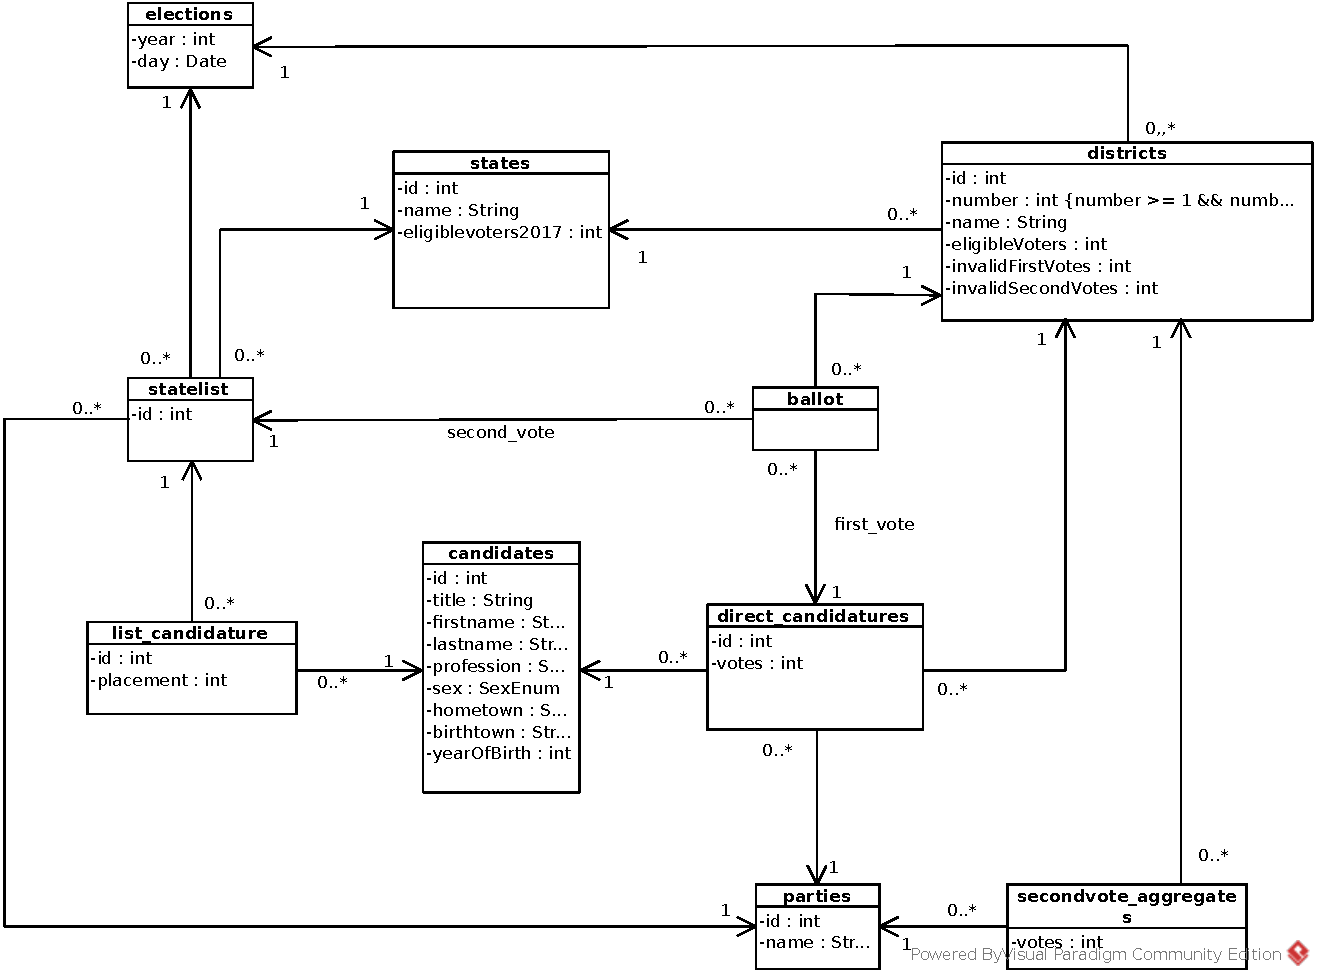
\includegraphics[width=\textwidth]{images/DBS_Schema.pdf}
\caption {Datenbank-Schema}
\end{figure}

\subsection{Server}

Für Entwicklungszwecke genügt der Server von IntelliJ.
Um diesen zu verwenden muss das Projekt in IntelliJ importiert werden, IntelliJ kann mit GWT als Framework von Haus aus umgehen.

\subsection{Client}

Der Client benötigt lediglich einen aktuellen Browser und kann die Anwendung sofort benutzen.

\subsection{Vorbereiten einer Wahl}

Zur Vorbereitung müssen Tokens erzeugt werden.
Diese werden mit Hilfe des Java-Projekts \texttt{token-gen}, welches im Projektordner liegt, generiert.
Die Main-Klasse muss mit den Argumenten \texttt{<n> <l1> <l2>} aufgerufen werden, wobei \texttt{n} durch die Anzahl der Wahlberechtigten und \texttt{l2} durch die benötigte Länge des Tokens zu ersetzen ist.
\texttt{l1} ist ein Parameter, mit dem die RAM-Auslastung kontrolliert werden kann
\footnote{
	Technischer Hintergrund:
	Die Tokens werden beim Generieren auf Duplikate geprüft.
	Da bei vielen Wahlberechtigten und wenig RAM nicht alle Tokens gleichzeitig im RAM vorgehalten werden können, wird die Generierung auf verschiedene Token-Präfixe verteilt.
	Die Länge des verwendeten Präfixes ist durch diesen Parameter gegeben.
},
der Parameter muss zwischen (jeweils einschließlich) \texttt{0} und \texttt{n} liegen.
Ein höherer Parameter bedeutet hierbei eine geringere RAM-Last.
Allerdings kompromittiert ein hoher Parameter die Sicherheit der Tokens.
Dabei kann für gegebene Parameter der Sicherheitsverlust wie folgt berechnet werden:
Mit $k = \mathrm{floor}(\frac{n}{36^{l1}})$ verringert sich die Sicherheit um $100\cdot k$\%.
Wenn ein Computer mit ausreichend RAM zur Verfügung steht, empfiehlt es sich also, $l1 = 0$ zu wählen.

Das Generieren und Einfügen von 50 Millionen Tokens in die Datenbank dauert je nach Hardware ungefähr 5 bis 10 Minuten.

\section{Benutzeroberfläche}

Die Benutzeroberfläche bietet einem Nutzer die Möglichkeit, sich über die Ergebnisse einer Bundestagswahl zu informieren. Dabei werden die Daten in einem einfachen, verständlichen Format angezeigt

\subsection{Auswahl eines Wahljahres}

Das System kann die Ergebnisse der Bundestagswahlen von 2013 und 2017 anzeigen. Standardmäßig werden die Ergebnisse von 2017 angezeigt. Der Nutzer kann über Checkboxen auswählen, welche Ergebnisse angezeigt werden sollen. Dem System liegen allerdings nur Daten über die Kandidaten von 2017 vor. Deshalb können einige Ergebnisse, wie die prozentuale Anzahl von Frauen im Bundestag, für die Bundestagswahl von 2013 nicht angezeigt werden. In diesen Fällen wird stattdessen eine entsprechende Meldung gezeigt


\subsection{Neuaggregierung der Stimmen}

Um neu eingetragene Stimmen bei den angezeigten Wahlergebnissen zu berücksichtigen kann ein Nutzer die Neuaggregierung der Einzelstimmen über eine Checkbox auslösen. Nach Ende dieser Neuaggregierung werden alle bis zum Zeitpunkt dieser Aggregierung in das System eingetragene Stimmen für die Berechnung der Wahlergebnisse berücksichtigt.


\subsection{Parlament}

Unter 'Parlament' wird die Sitzverteilung im Bundestag angezeigt. Zudem sind dort die prozentuale Verteilung von Stimmen auf Parteien,  die Überhangmandate und die Mitglieder des Bundestags zu sehen. 

\begin{figure}[H]
\centering
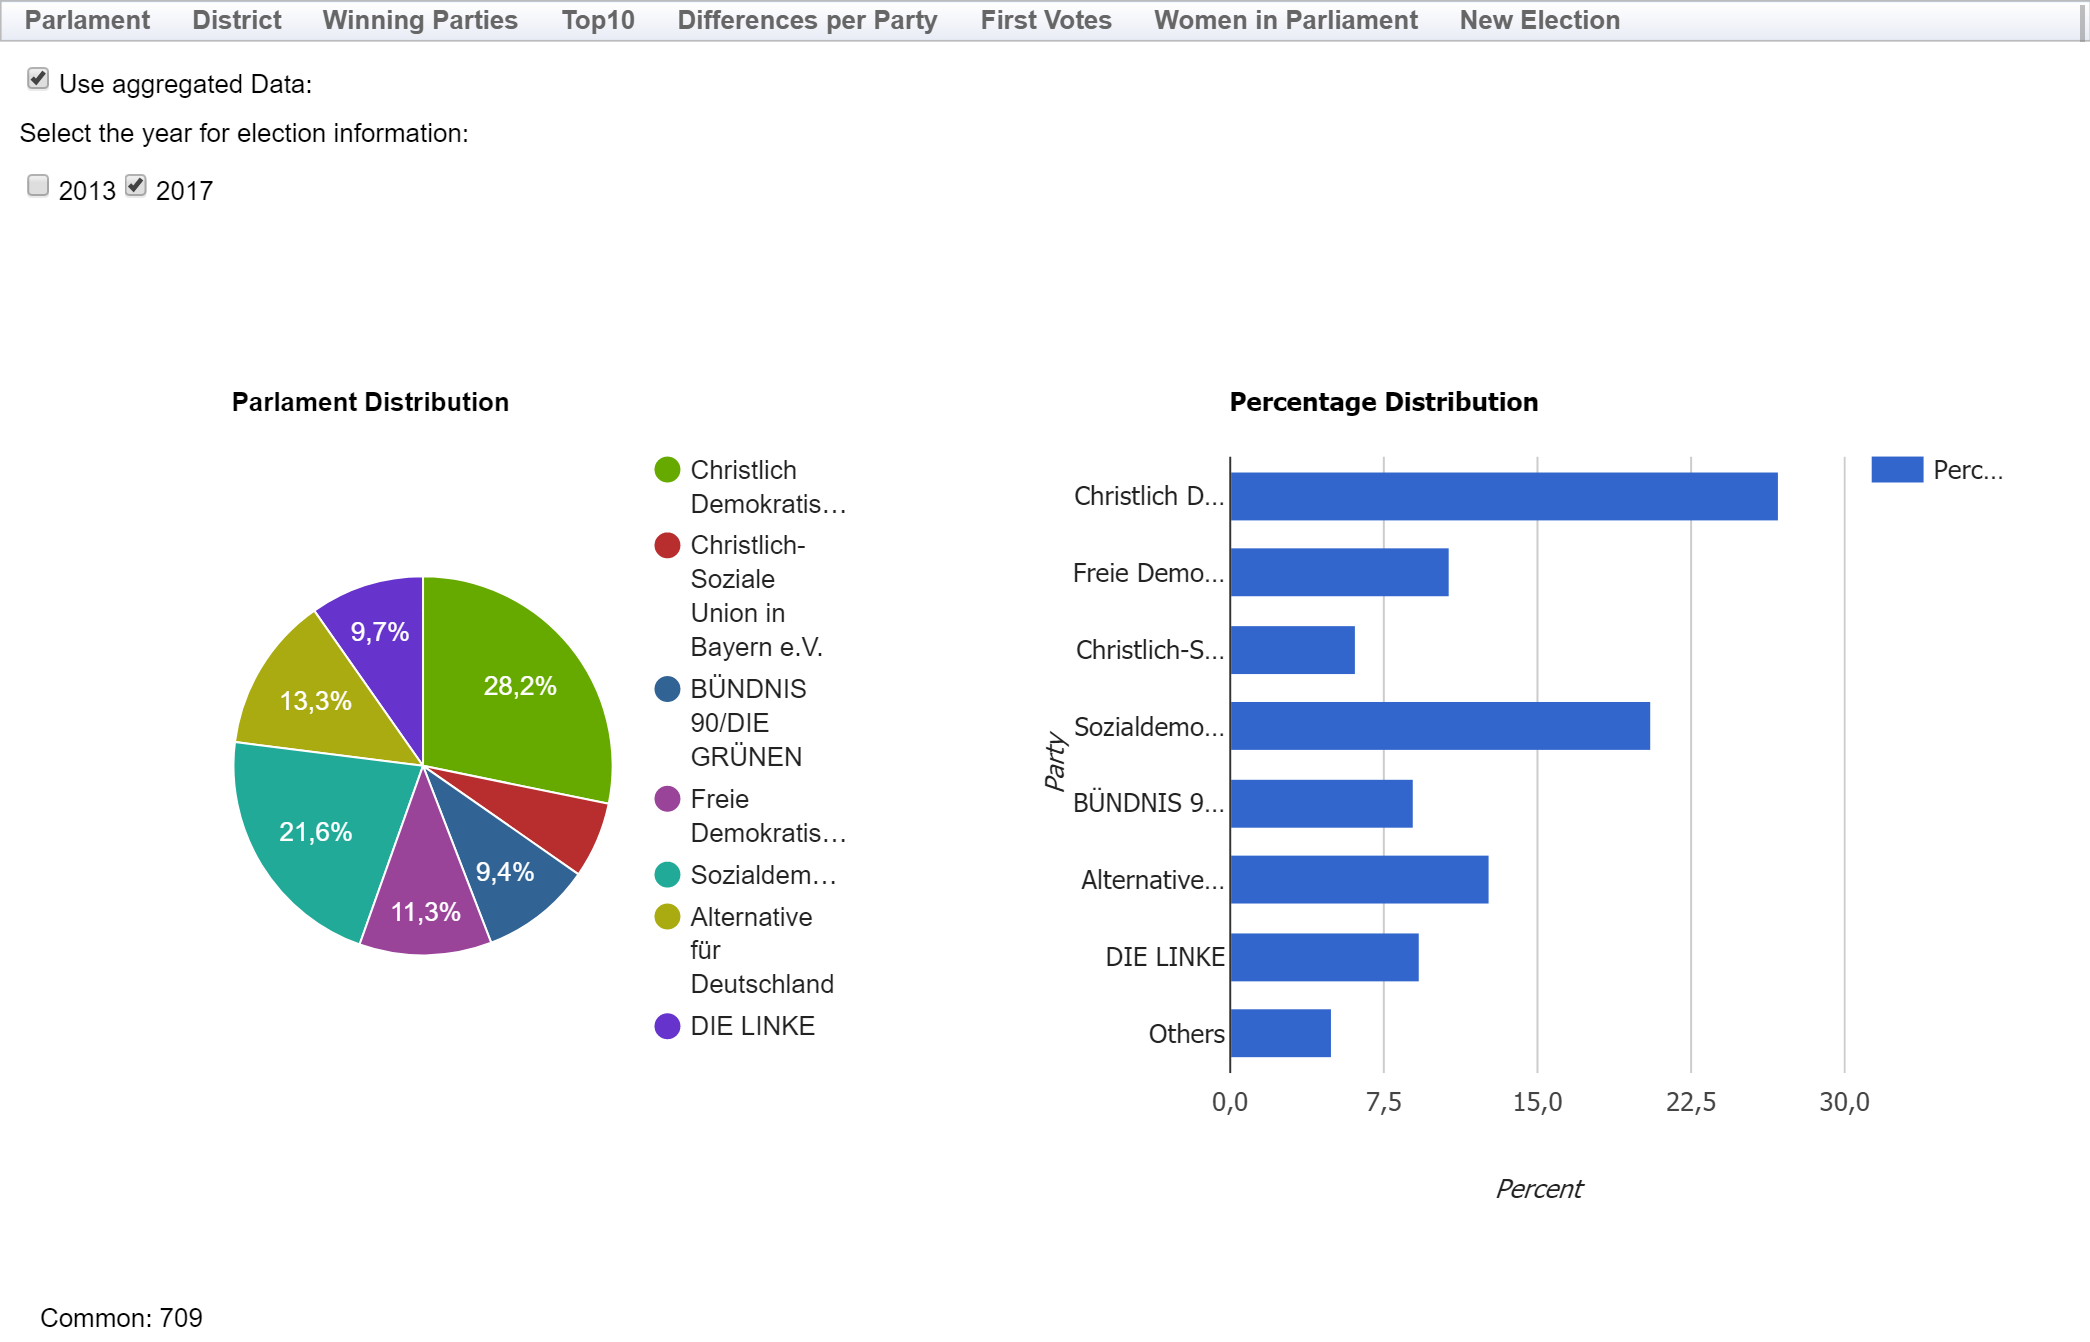
\includegraphics[width=\textwidth]{images/parliament_distribution.png}
\caption {Parliament distribution}
\end{figure}

\begin{figure}[H]
\centering
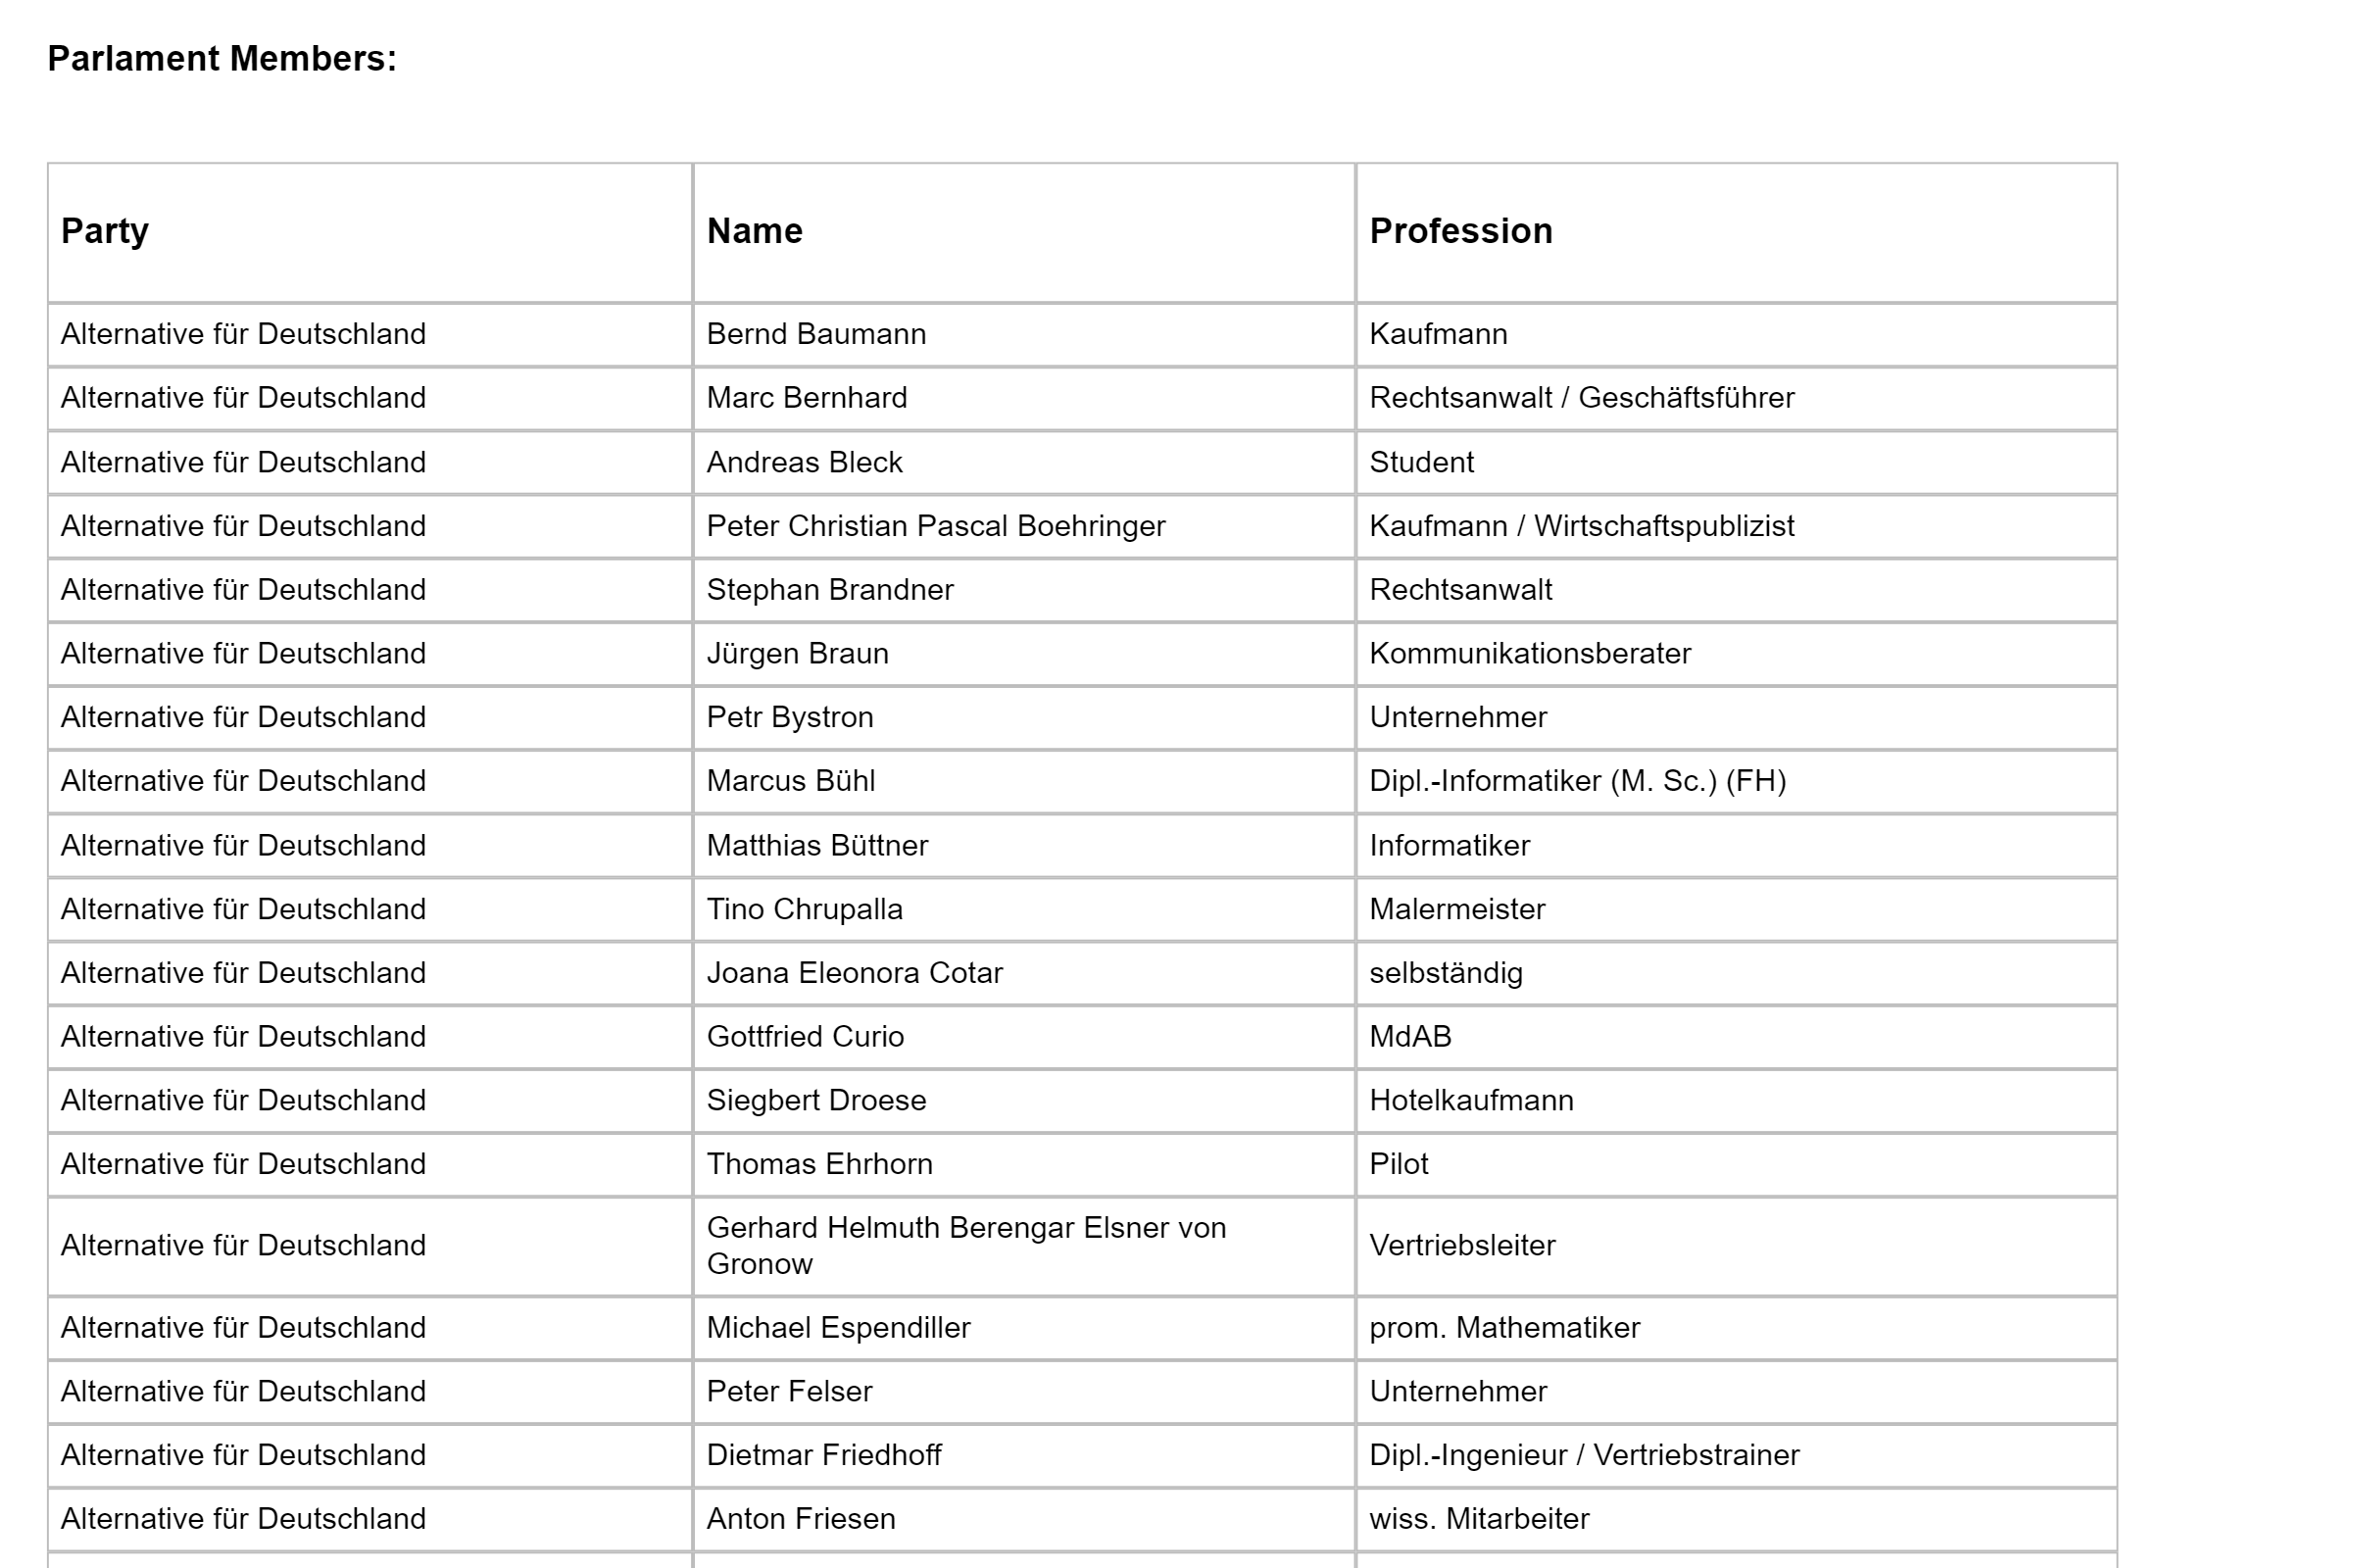
\includegraphics[width=0.8\textwidth]{images/parliament_members.png}
\caption {Parliament members}
\end{figure}

\begin{figure}[H]
\centering
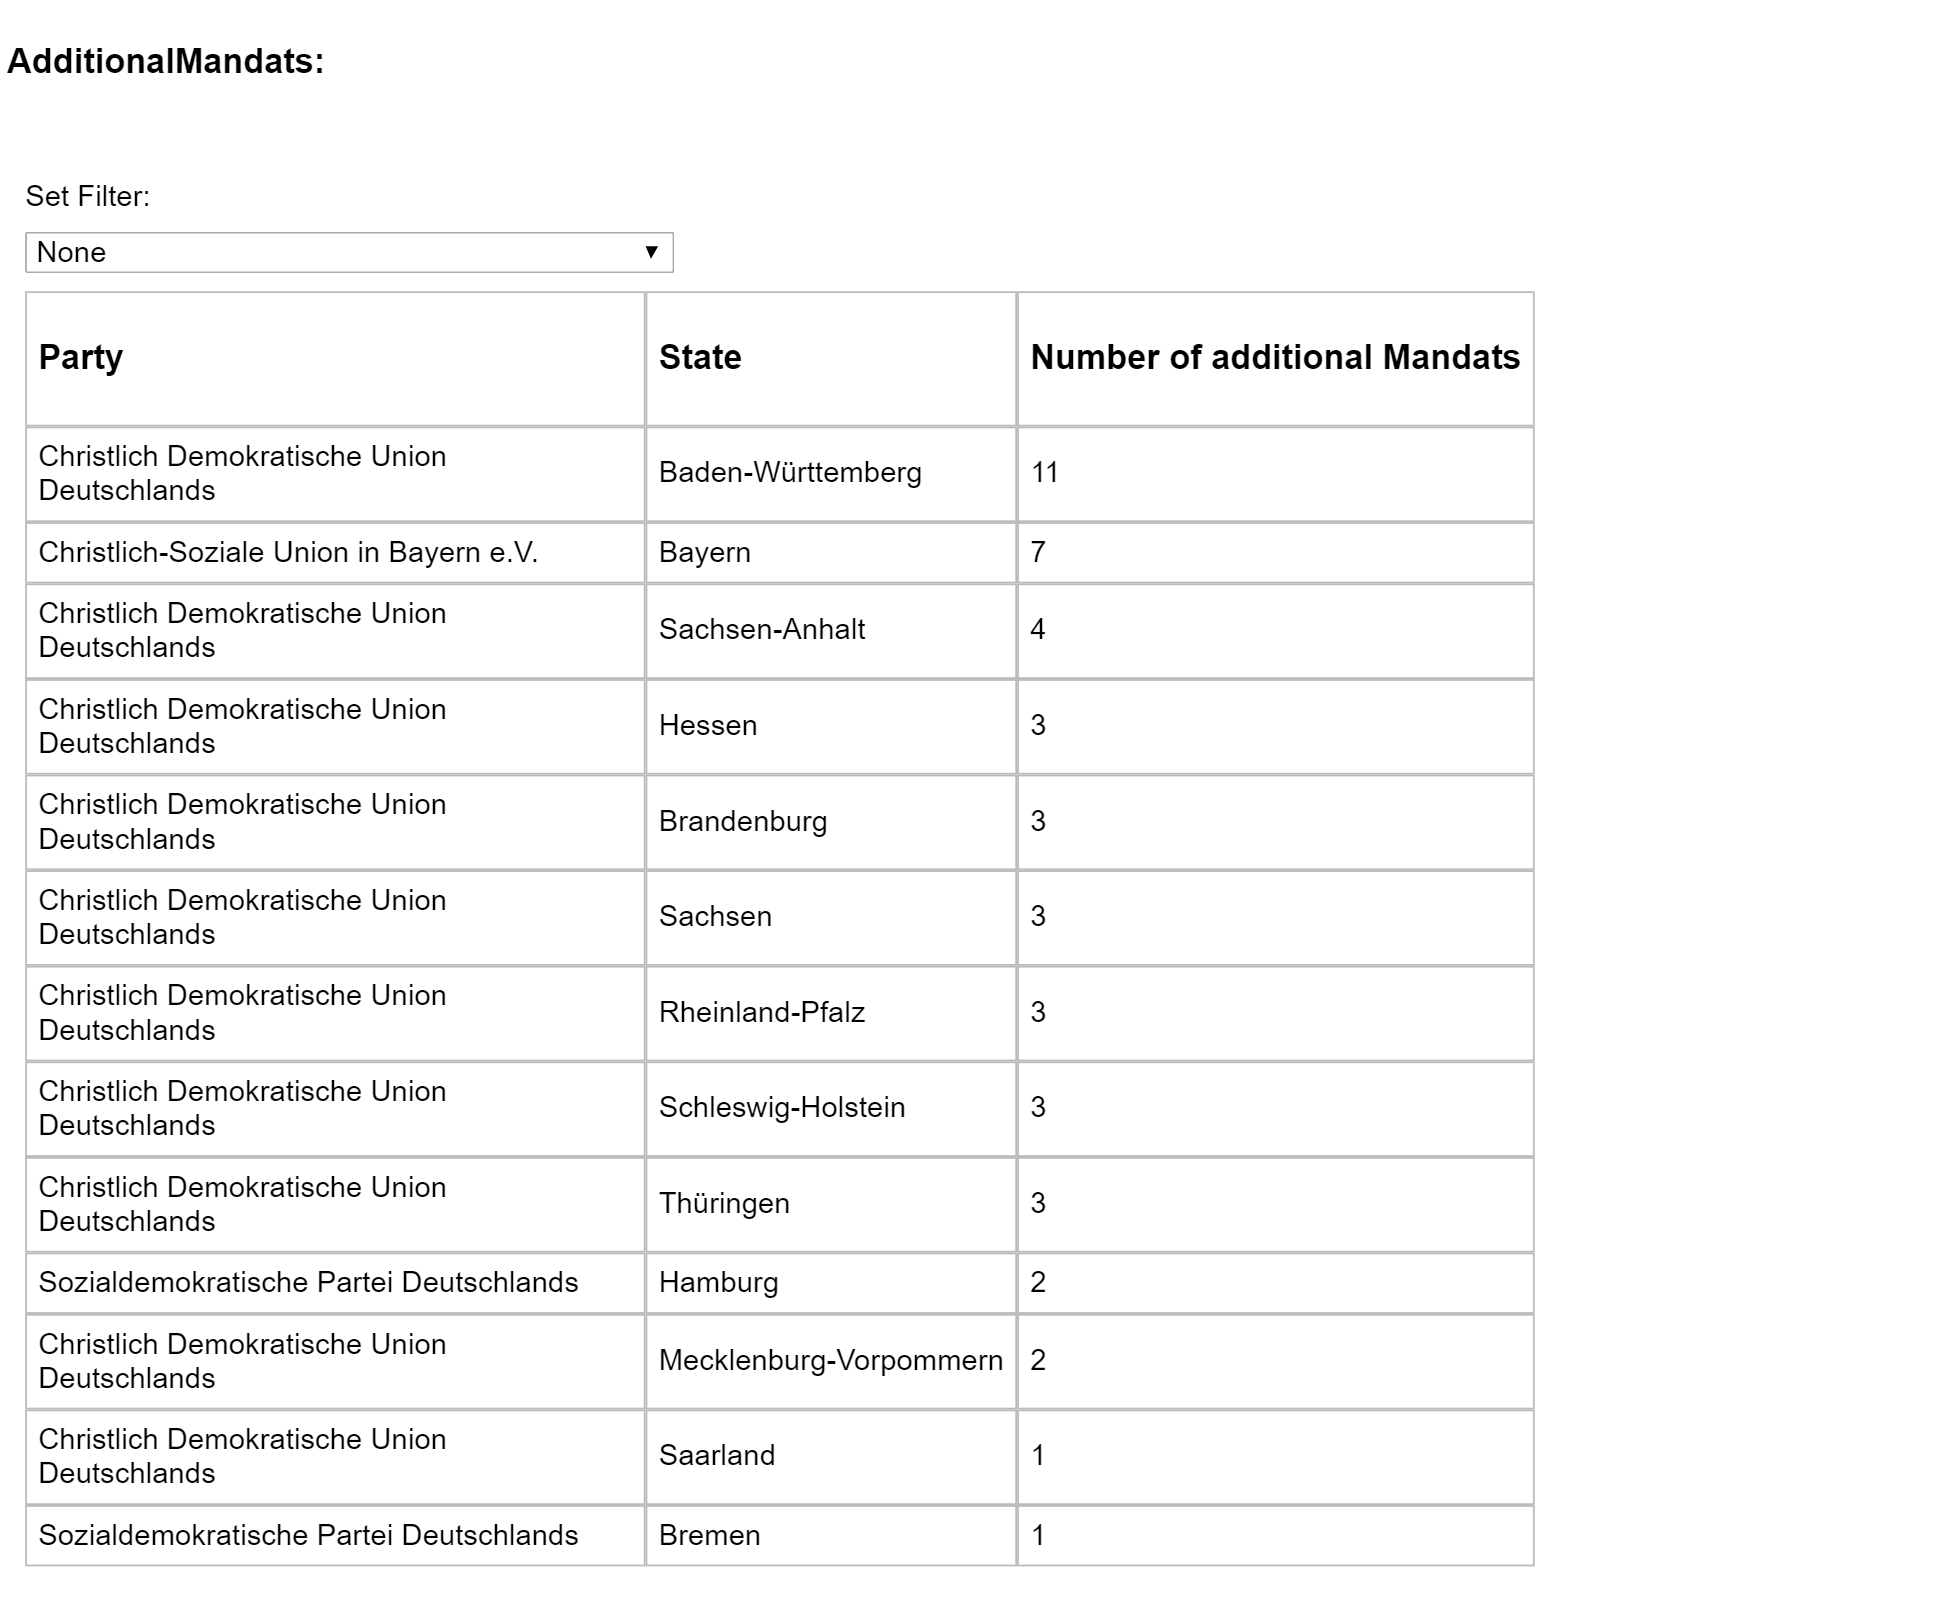
\includegraphics[width=\textwidth]{images/additional_mandats.png}
\caption {Additional mandats}
\end{figure}

\subsection{District}

Unter 'District' wird die Anzahl von Wählern und Nichtwählern und die Verteilung von Erst- und Zweitstimmen auf Parteien angezeigt. Diese Daten werden jeweils im Vergleich zu den Daten der vorherigen Bundestagswahl dargestellt. Da das System keine Daten zur Bundestagswahl von 2009 enthält, gibt es hier keine eigene Anzeige für die Bundestagswahl von 2013. Die Ergebnisse von 2013 werden bei den Daten von 2017 als Vergleich mit angezeigt.

\begin{figure}[H]
\centering
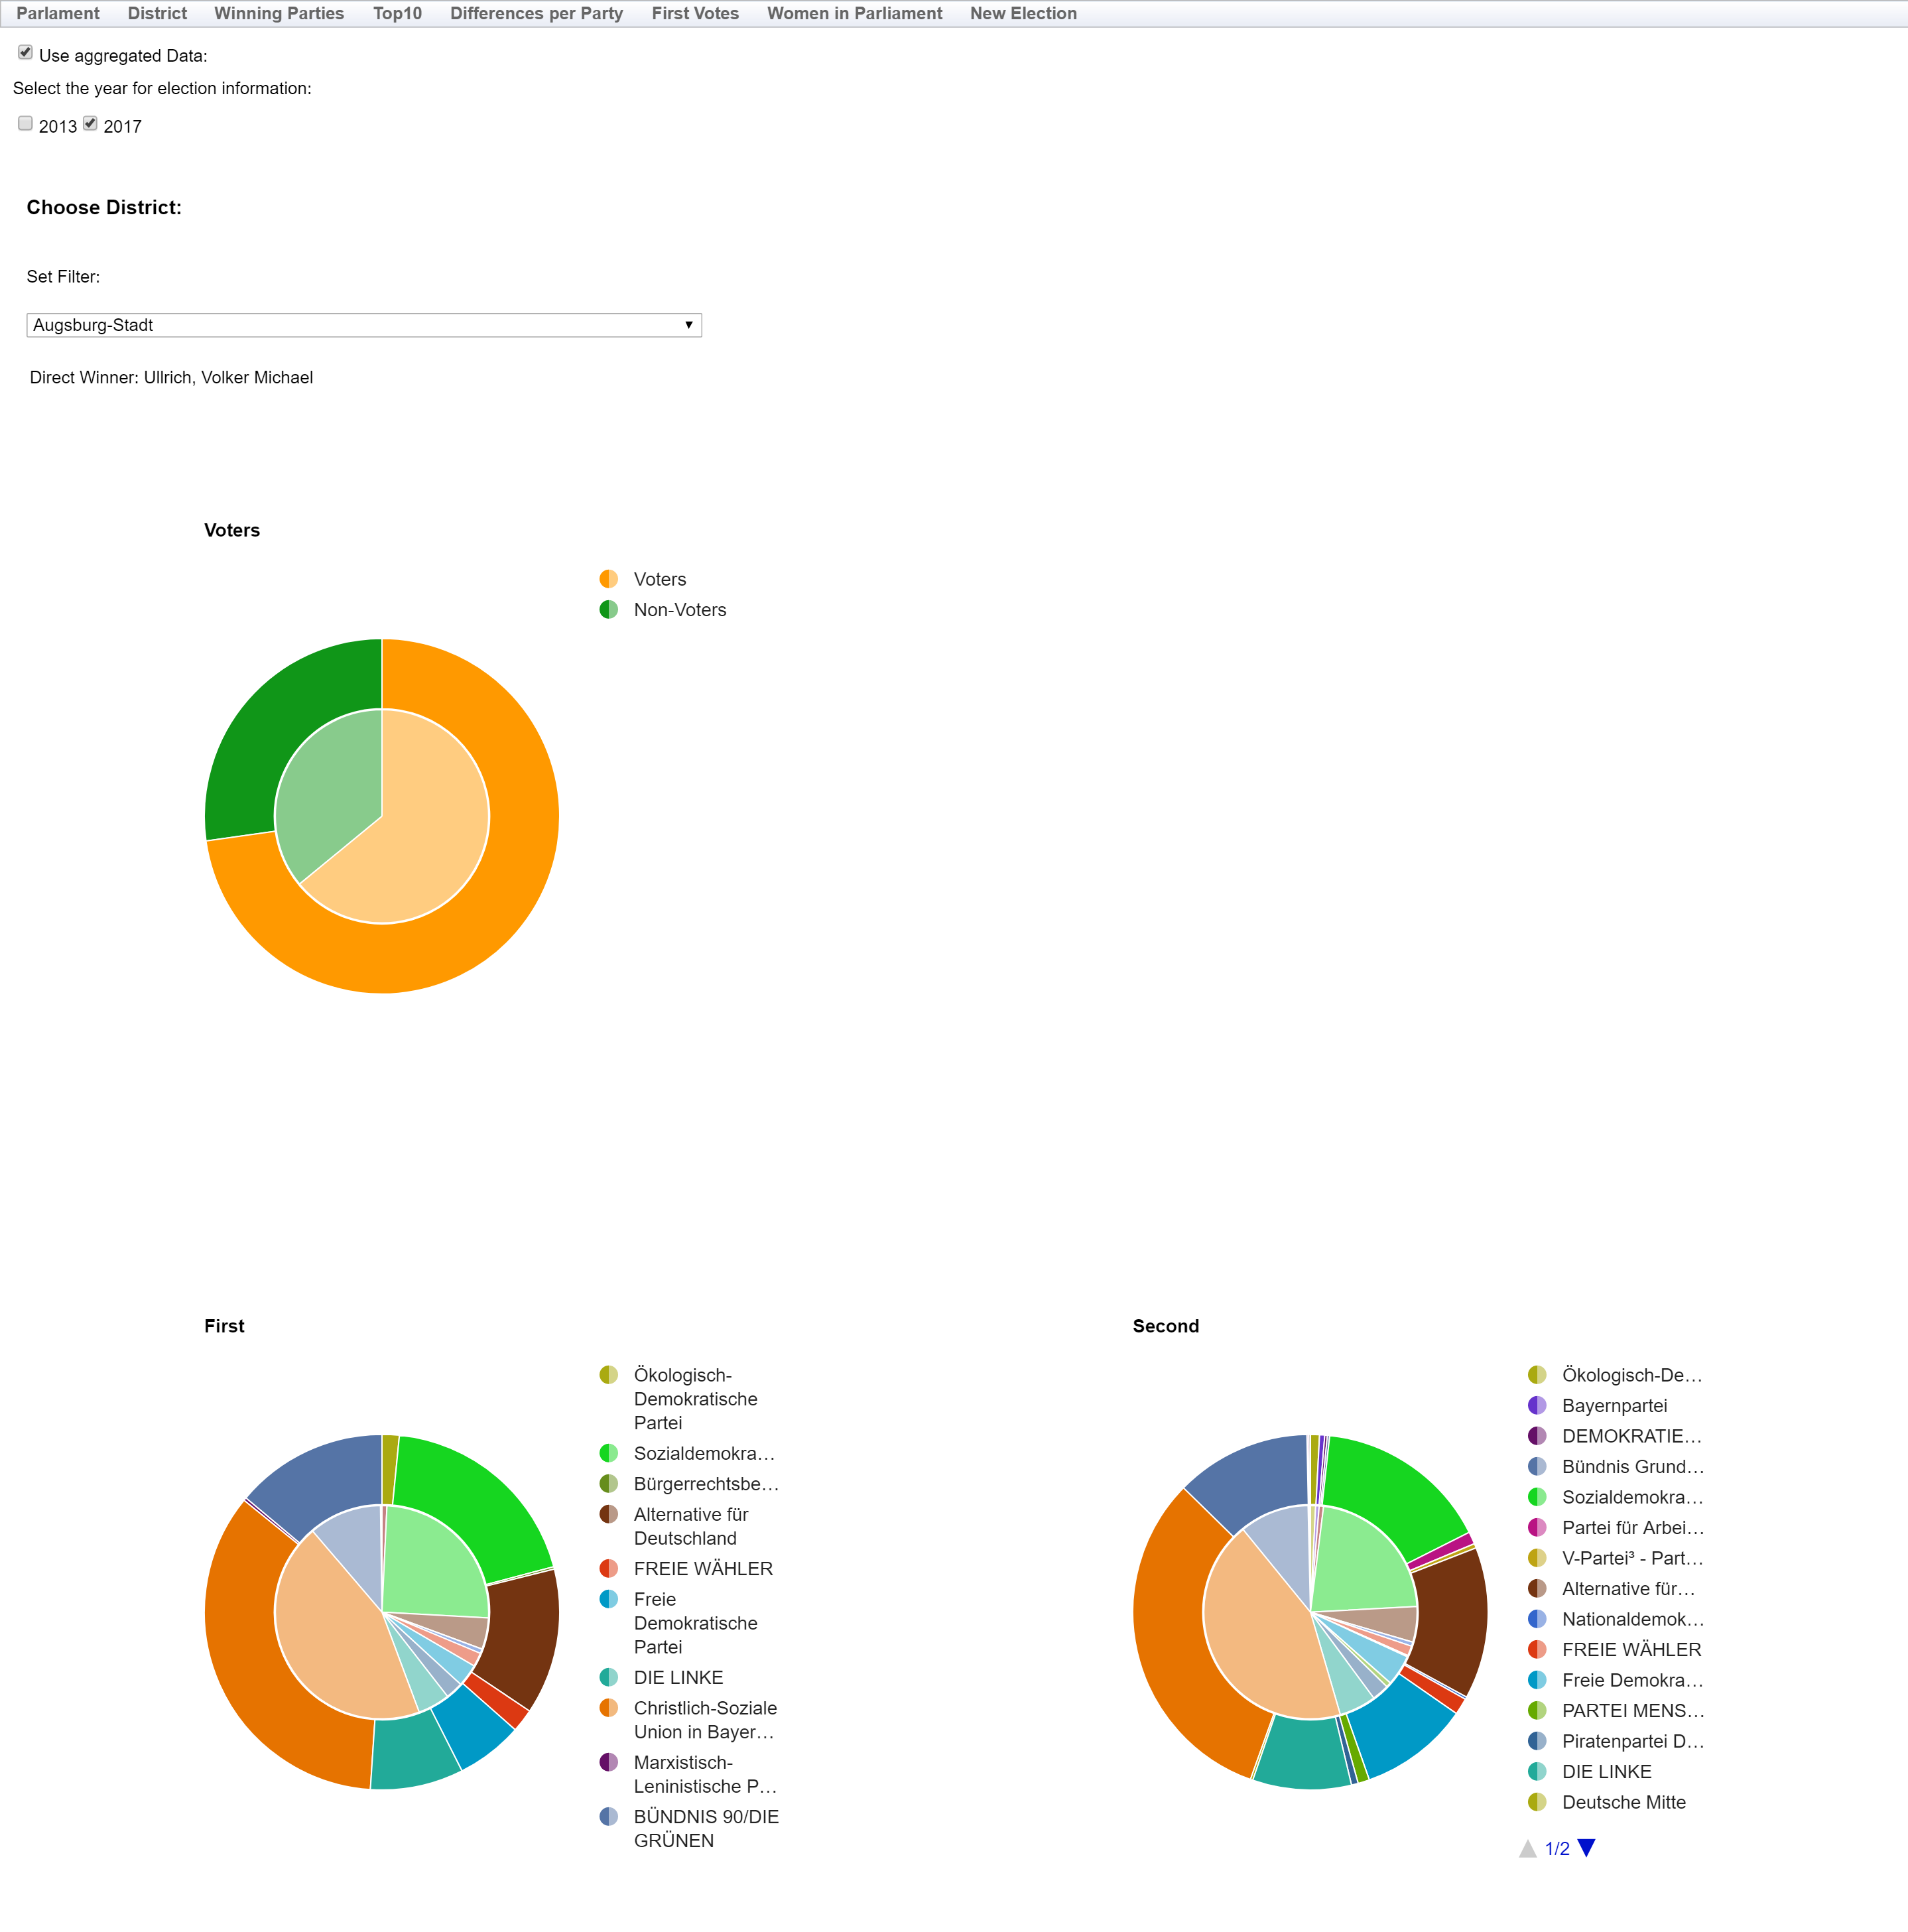
\includegraphics[width=\textwidth]{images/district.png}
\caption {District view}
\end{figure}

\subsection{Top10}

Unter 'Top 10' werden -- pro Partei -- die knappsten Gewinner und Verlierer bezüglich der Erststimmen angezeigt.
Hierbei werden die Gewinner und die "`Verlierer"', also die zweitplatzierten Kandidaten, berücksichtigt.
Angezeigt werden solche Kandidaten, die bundesweit am knappsten gegen die Konkurrenz gewonnen oder verloren haben.
Diese Information ist besonders für die Parteien interessant: In diesen Wahlkreisen lohnt sich der Wahlkampf am meisten.

\begin{figure}[H]
\centering
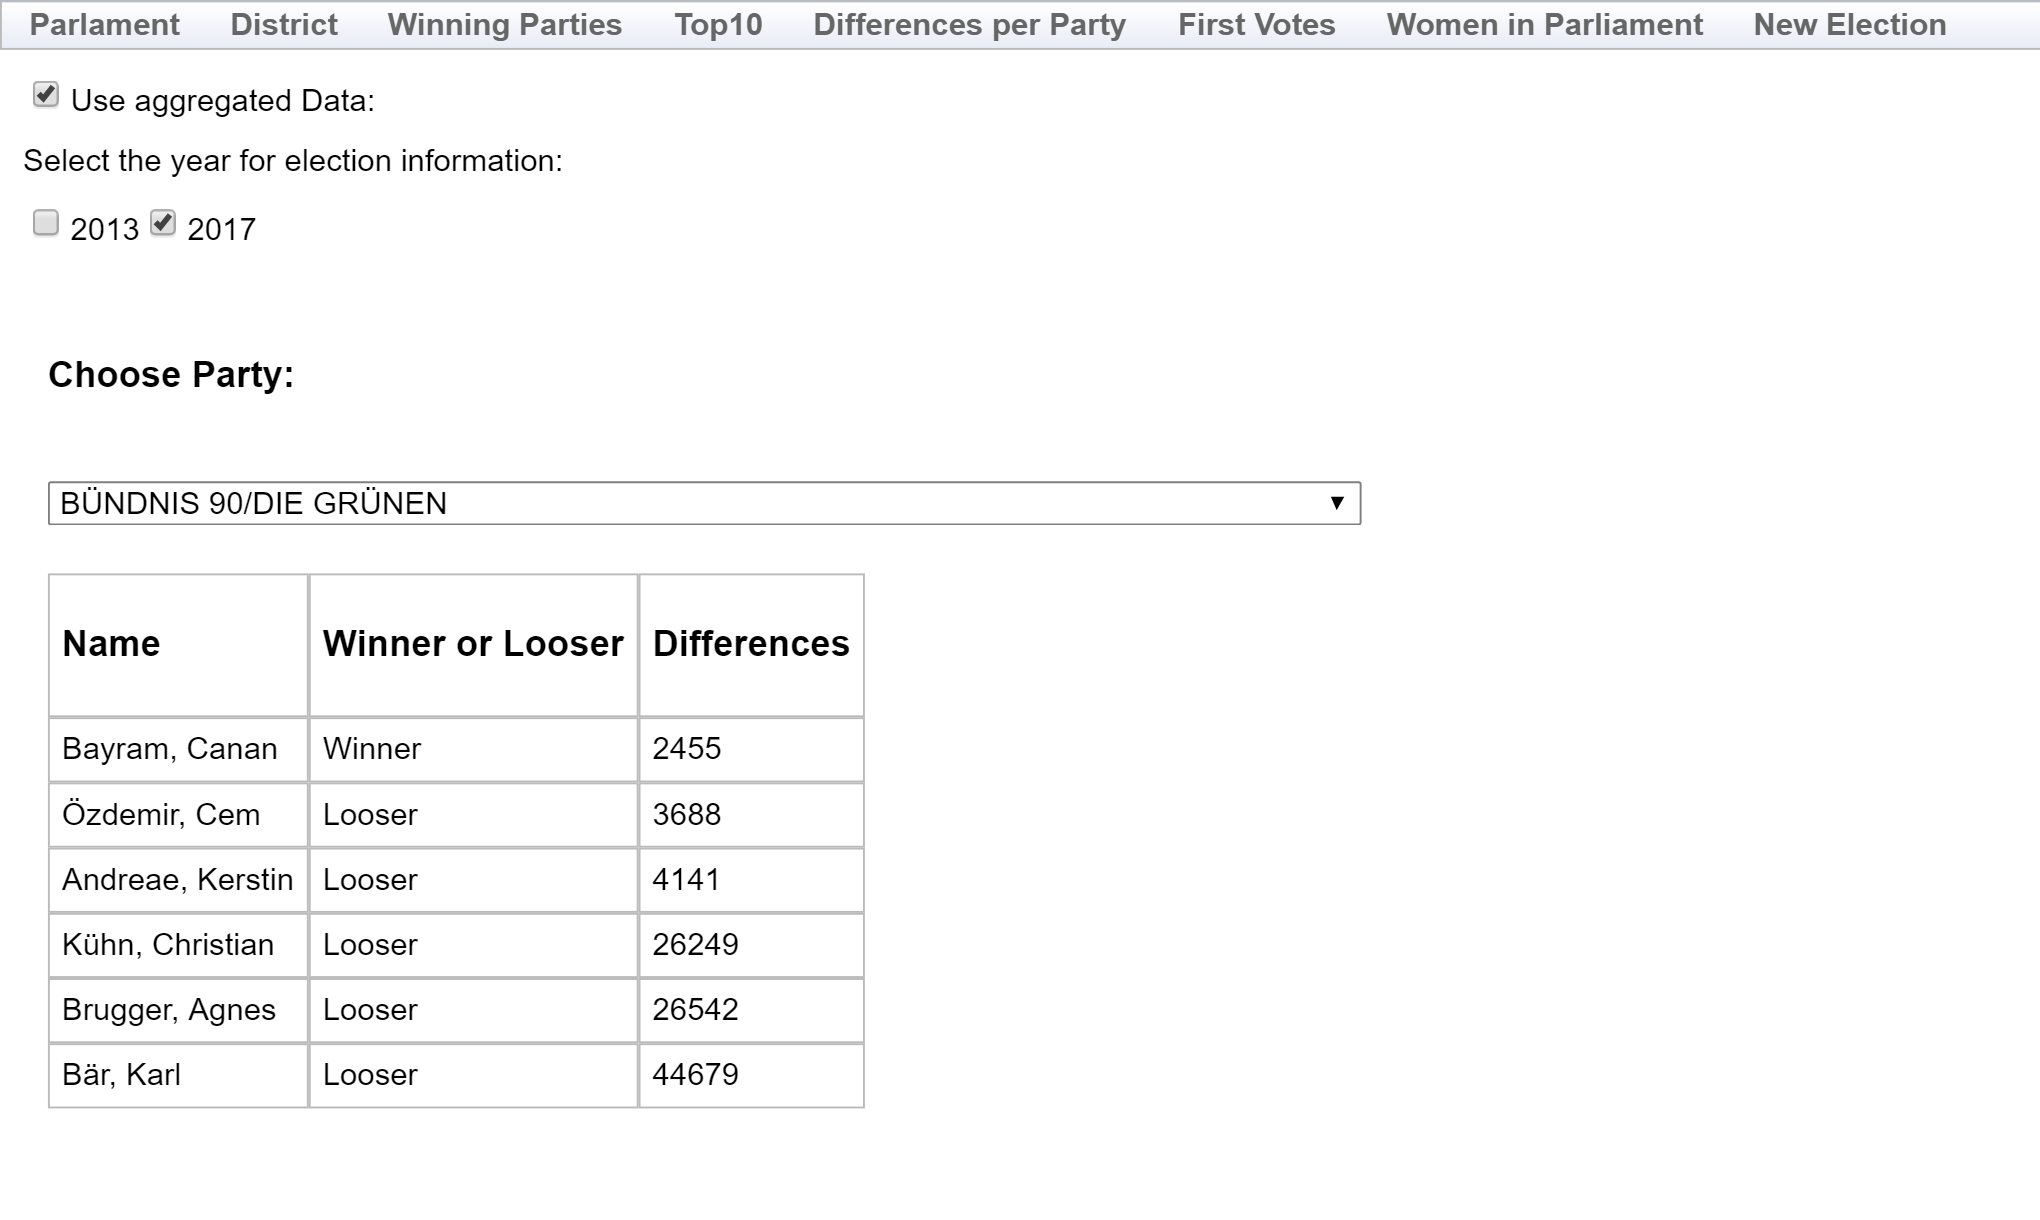
\includegraphics[width=\textwidth]{images/top10.png}
\caption {Top 10 view}
\end{figure}

\subsection{Difference First Second Votes}

Unter 'Difference First Second Votes' wird für jede Partei einer Bundestagswahl angezeigt, in welchem Wahlkreis der Abstand zwischen ihrer Erst- und Zweitstimmen am größten war. Die Größe dieses Abstands wird als Balkendiagramm angezeigt. Wenn der Nutzer mit der Maus über eine dieser Balken fährt kann er sehen, in welchem Wahlkreis der Abstand zwischen den Erst- und Zweitstimmen der Partei am größten war und ob sie mehr Erst- oder mehr Zweitstimmen erhalten haben. Daran kann man sehen, ob ein bestimmter Erstkandidat besonders beliebt oder besonders unbeliebt war, oder ob der Erstkandidat wenig Einfluss auf die Anzahl der erhaltenen Erststimmen hatte. Zudem kann geprüft werden, ob an sehr kleine oder sehr große Parteien bevorzugt Erst- oder Zweitstimmen vergeben werden. 

\begin{figure}[H]
\centering
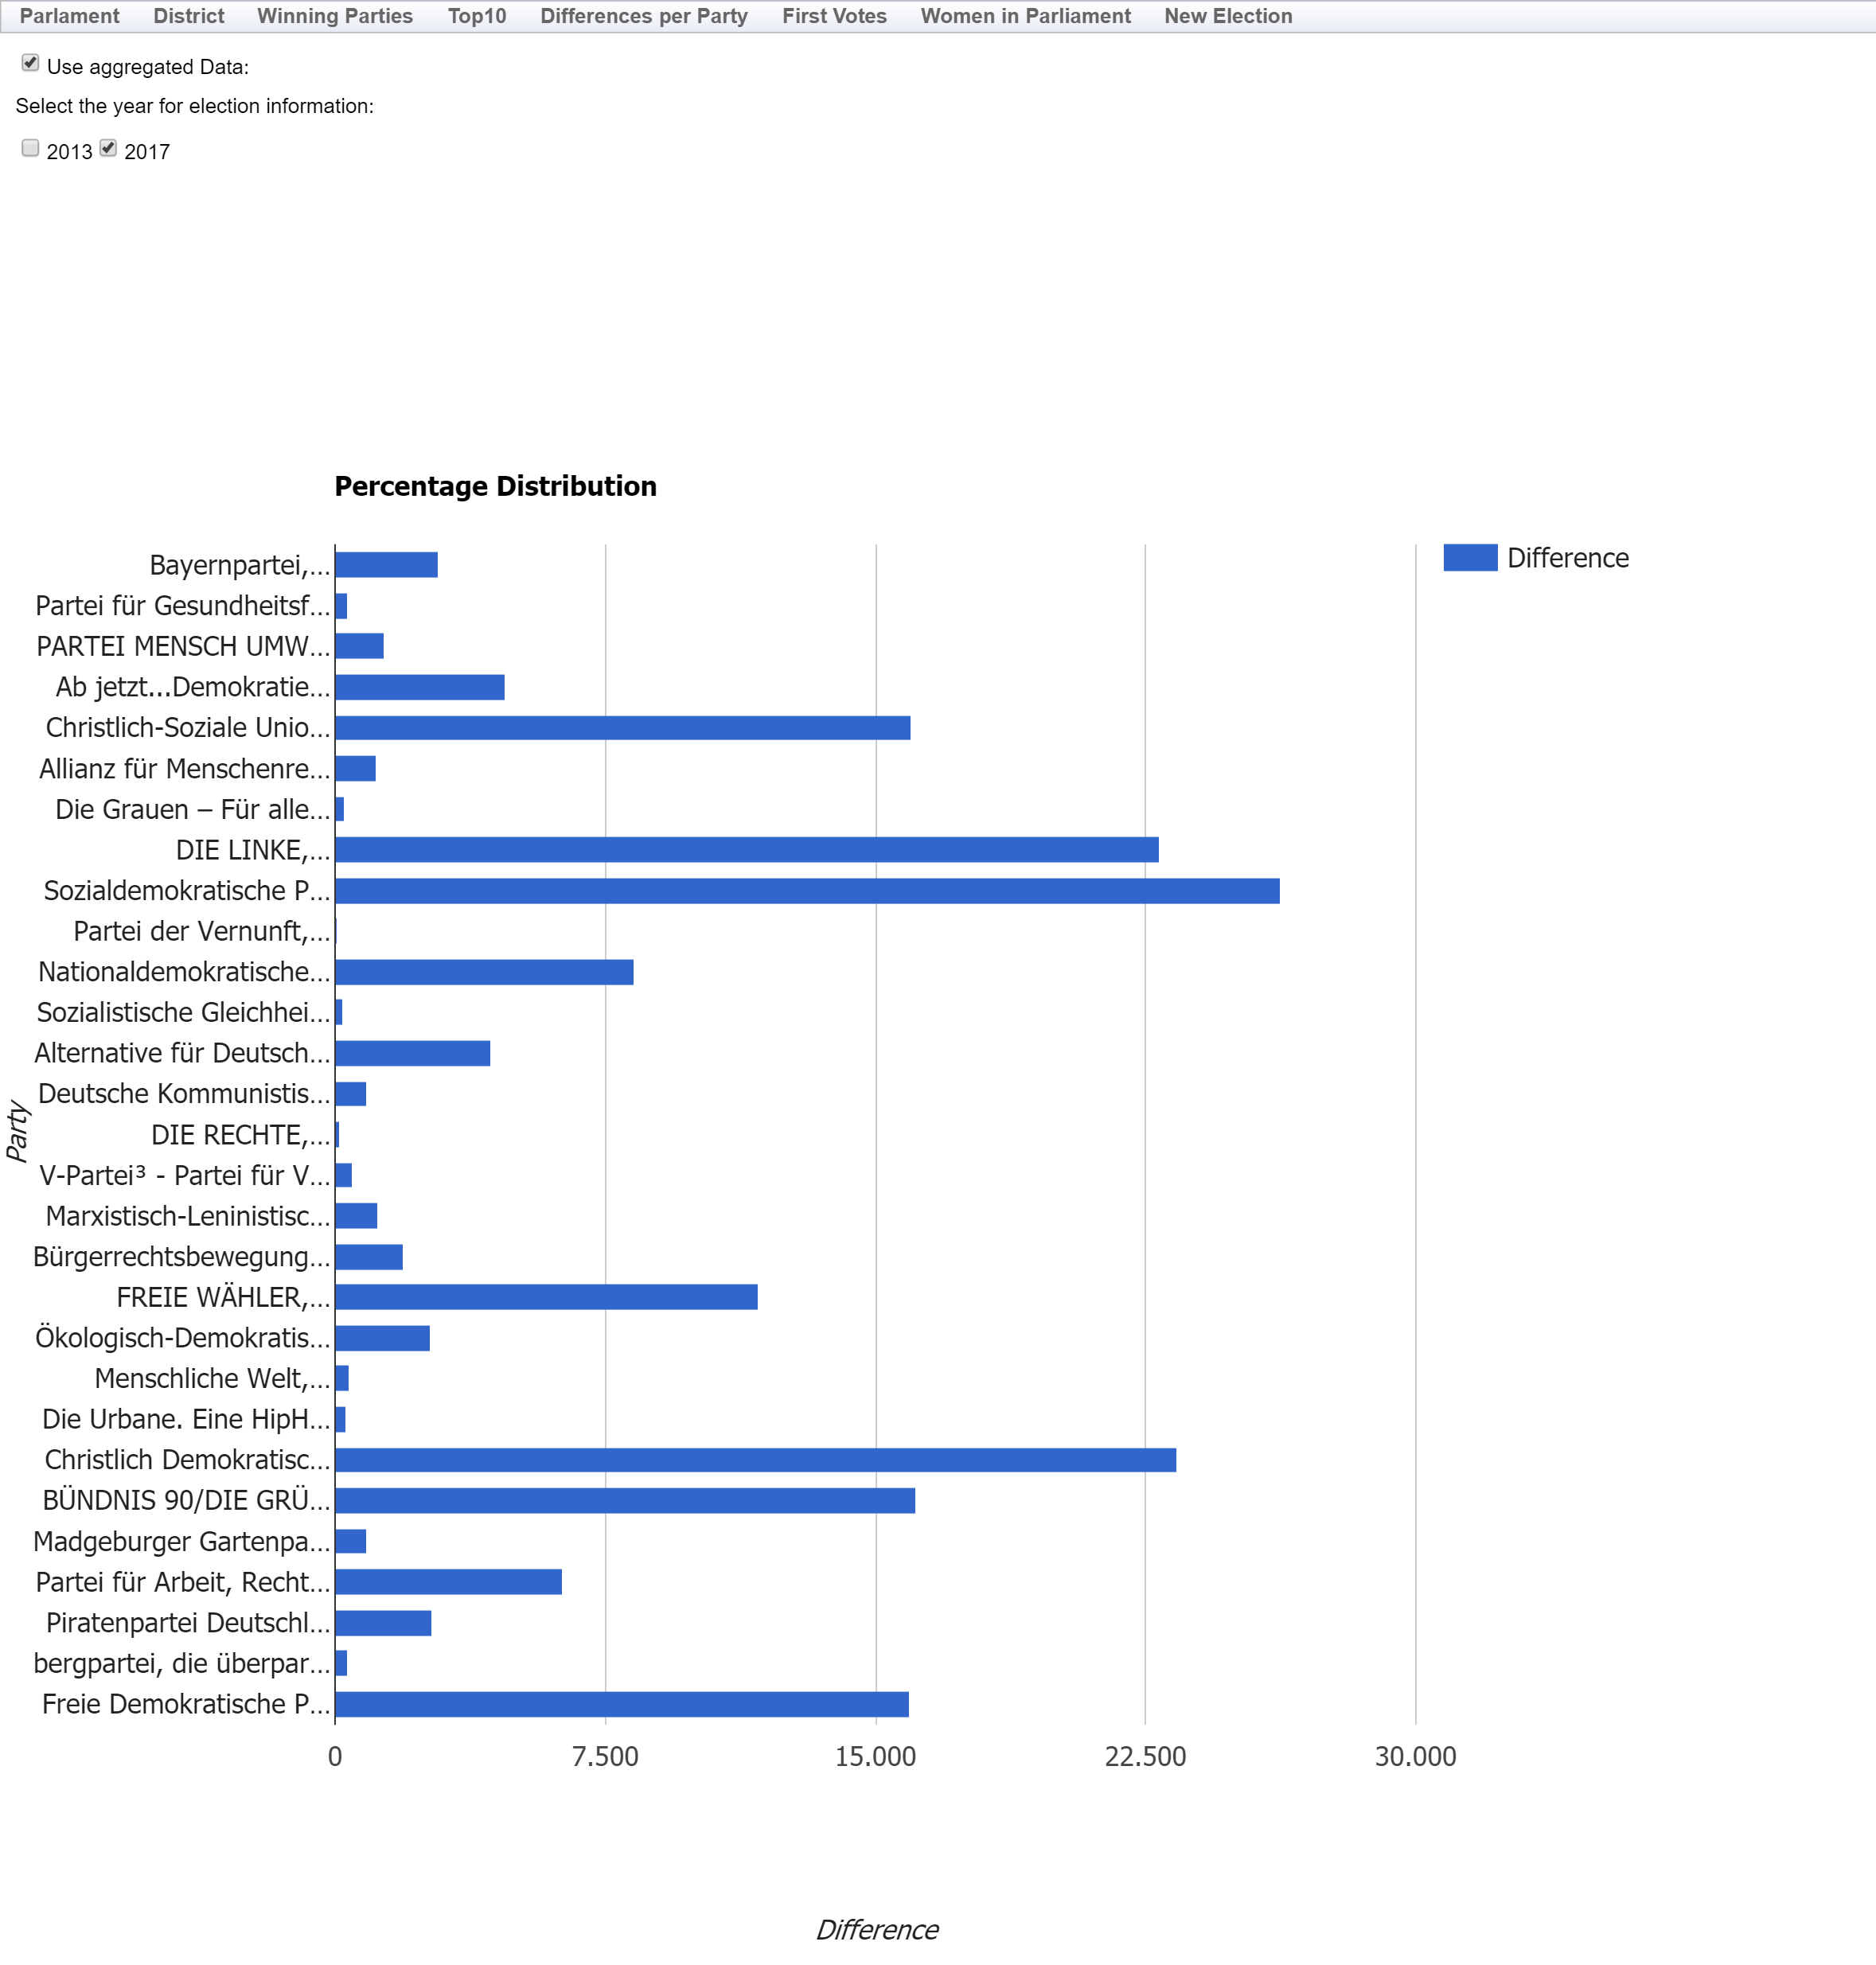
\includegraphics[width=\textwidth]{images/diffrences_per_party.png}
\caption {Differences per party}
\end{figure}

\subsection{First Votes}

Unter 'First Votes' wird die Verteilung der Erststimmen auf Bundestagsebene angezeigt. Hier kann der Nutzer sehen, ob eine stärkere Gewichtung der Erststimmen das Ergebnis einer Bundestagswahl beeinflussen könnte.

\begin{figure}[H]
\centering
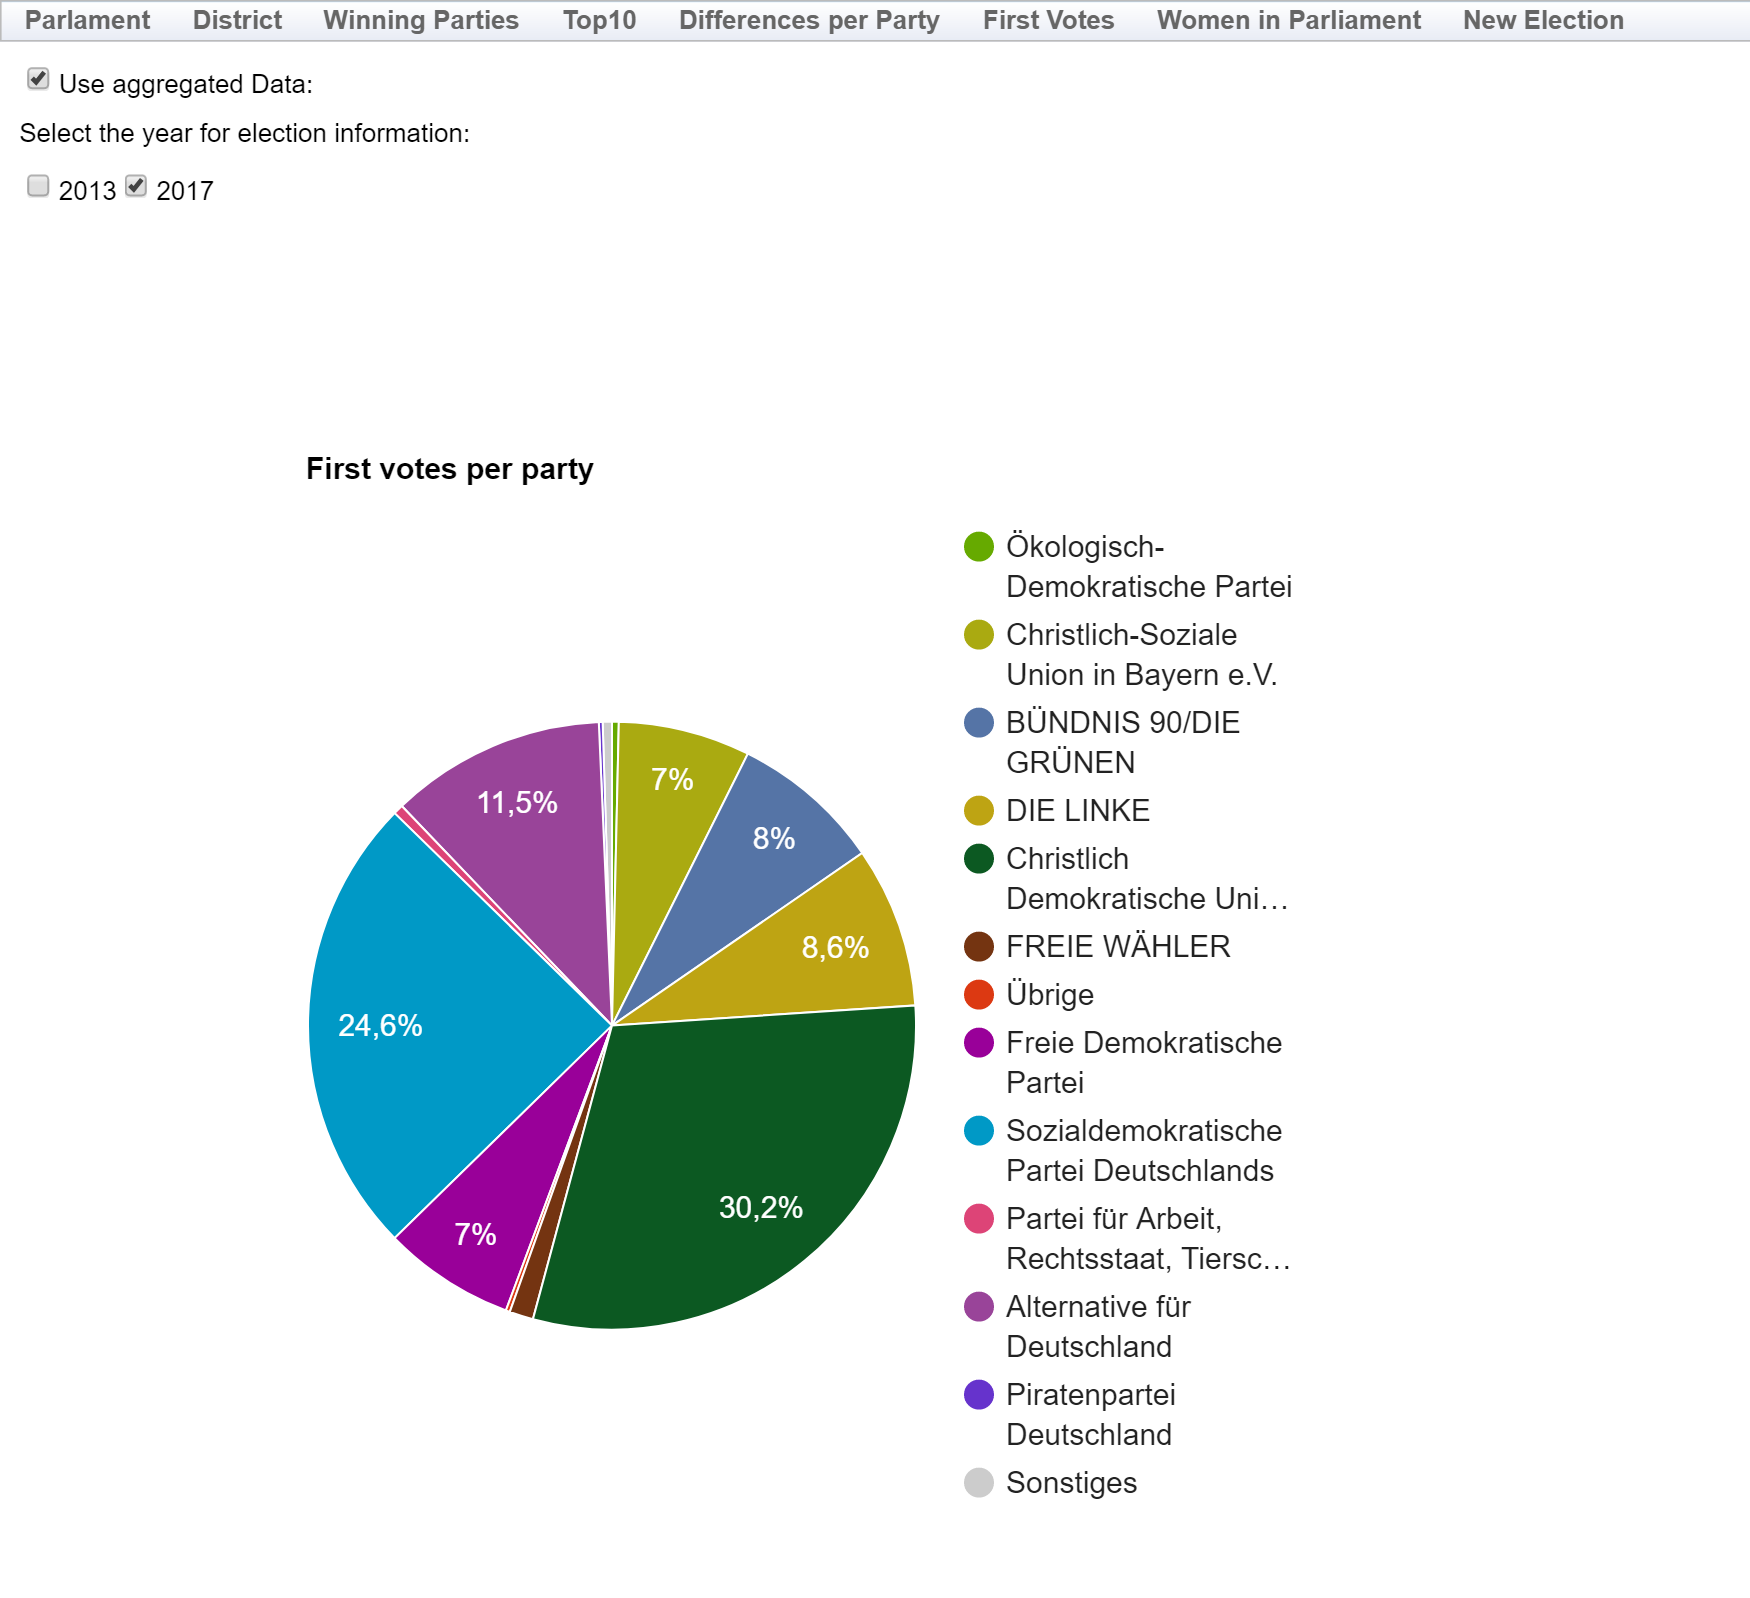
\includegraphics[width=\textwidth]{images/first_votes.png}
\caption {First votes view}
\end{figure}

\subsection{Women in Parliament}

Unter 'Women in Parliament' wird die prozentuale Anzahl der Frauen und Männer im Bundestag angezeigt. Da das System keine entsprechenden Daten über die Kandidaten von 2013 enthält ist diese Anzeige nur für die Bundestagswahl von 2017 möglich

\begin{figure}[H]
\centering
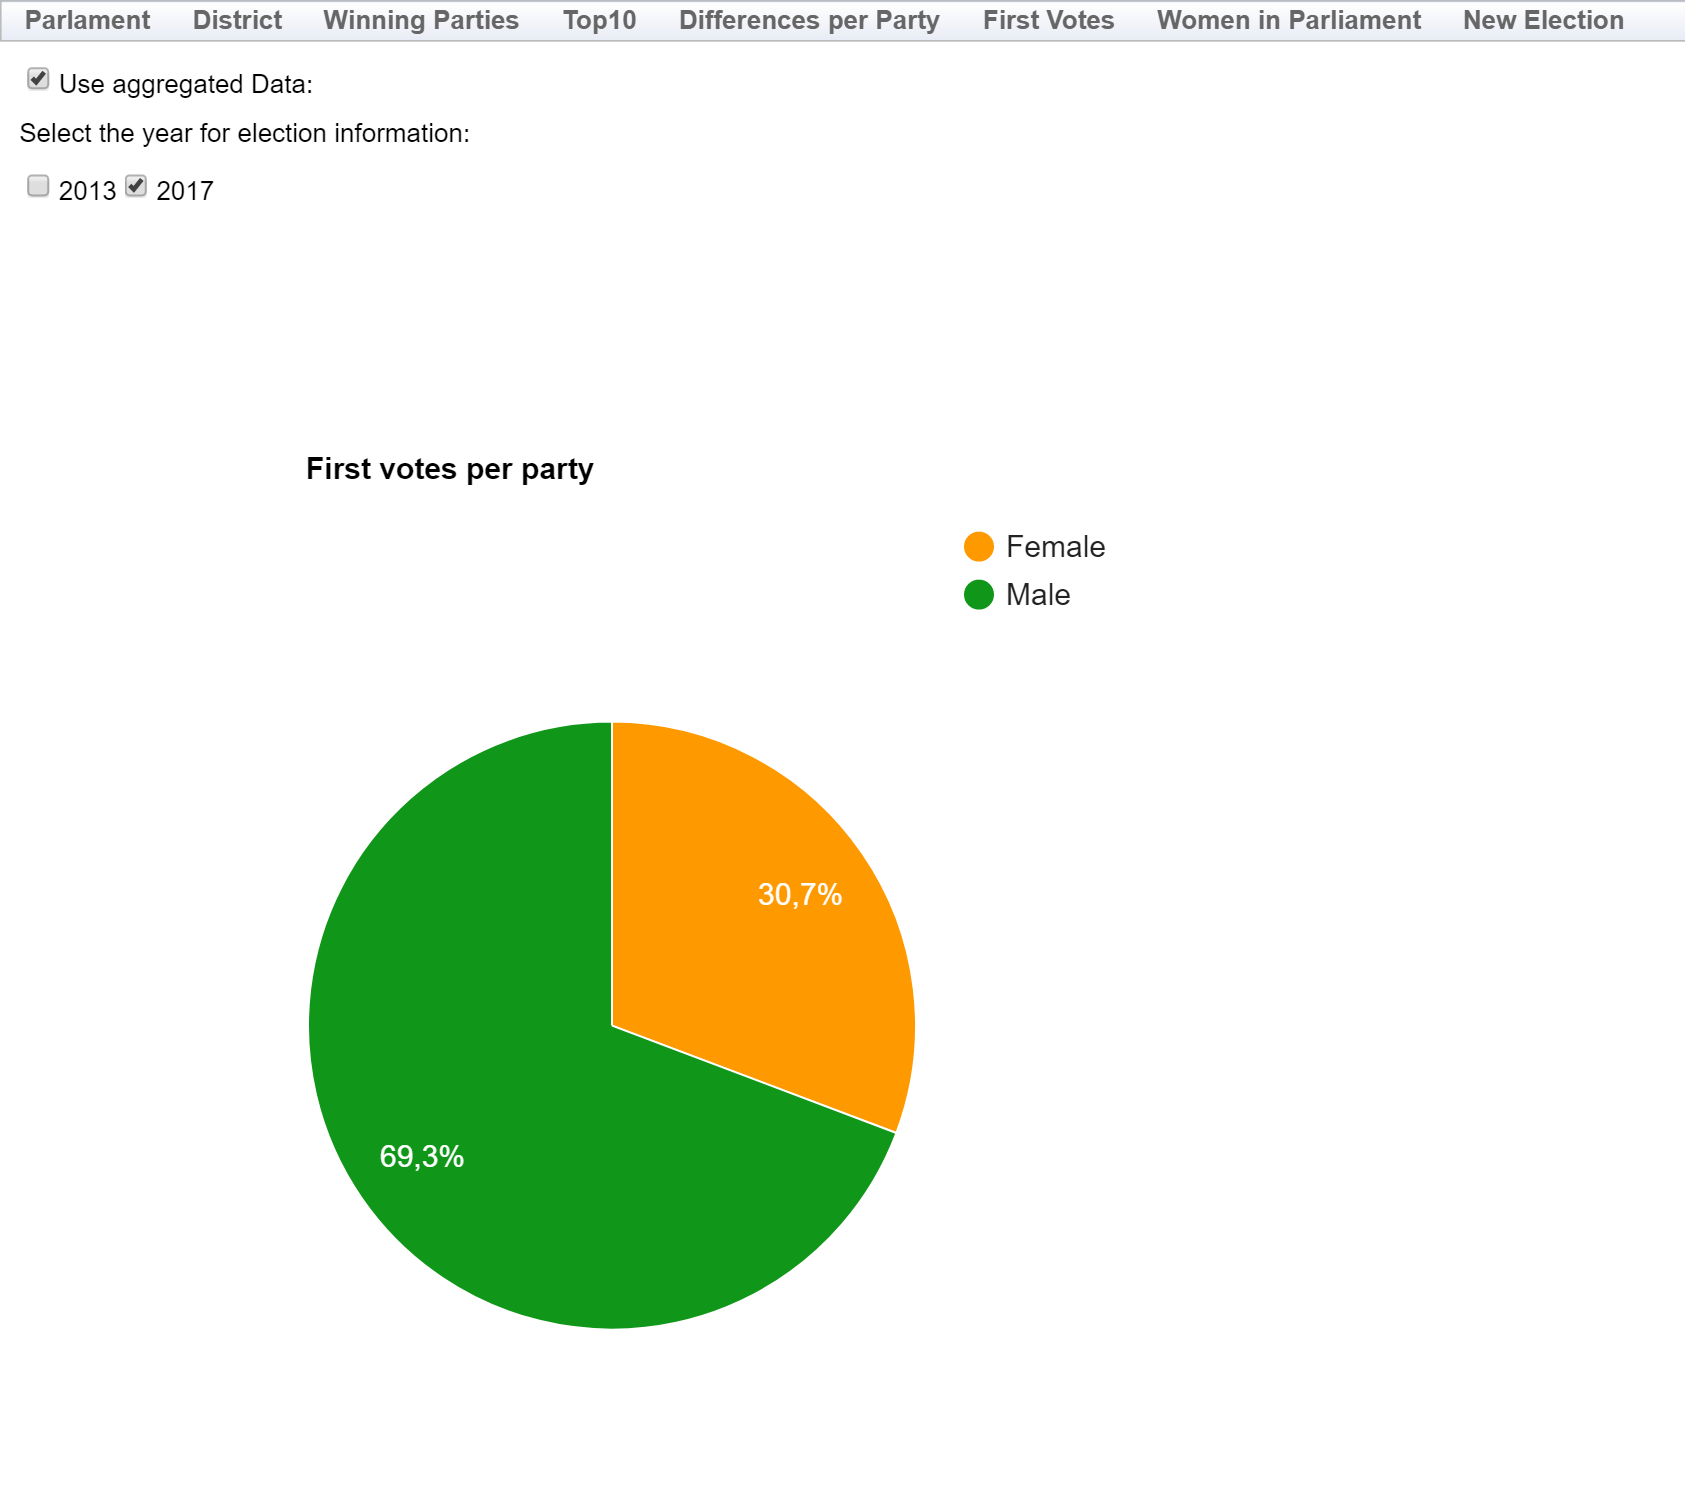
\includegraphics[width=\textwidth]{images/female_in_parliament.png}
\caption {Women in parliament view}
\end{figure}


\section{Berechnung der Ergebnisse}

Als Grundlage für die Berechnung dienen die Stimmverteilungen auf Wahlkreisebene, die auf https://www.bundeswahlleiter.de/ einsehbar sind. Hierbei werden für 2013 die Ergebnisse verwendet, die bei den Wahlergebnissen von 2017 enthalten sind. Diese Ergebnisse wurden auf die neu verteilten Wahlkreise für die Bundestagswahl von 2017 umgerechnet.

Die Berechnung der Ergebnisse der Bundestagswahlen, die von dem Wahlinformationssystem angezeigt werden, erfolgen ausschließlich über SQL-Anfragen. Eine kommentierte Version der verwendeten Anfragen ist dieser Dokumentation beigefügt. 


\section{Funktion zur Stimmenabgabe}

Das Wahlinformationssystem unterstützt eine Stimmabgabe-Funktion.
Dies ermöglicht es, ein Wahllokal auf digitale Wahl umzustellen, womit der Prozess der Stimmenauszählung automatisiert erfolgen kann.

\subsection{Vorbereitung des Systems für die Stimmenabgabe}

Zunächst müssen für eine Wahl Tokens erstellt werden.
Dies geschieht mit einem Kommandozeilenprogramm im Vorfeld.
Die Tokens werden daraufhin in der benötigten Menge für jedes Wahllokal gedruckt.

Im Wahllokal werden nun ein oder mehrere Wahlcomputer aufgebaut.
Diese müssen eine stabile Verbindung zum zentralen Backend-Server aufweisen.

In einem Browser wird nun die Weboberfläche des Wahlsystems geöffnet.
Auf der Website wird die Funktion 'New Election' gewählt.
Daraufhin wird eine Auswahlseite angezeigt, in der der Wahlkreis ausgewählt wird.

\begin{figure}[H]
\centering
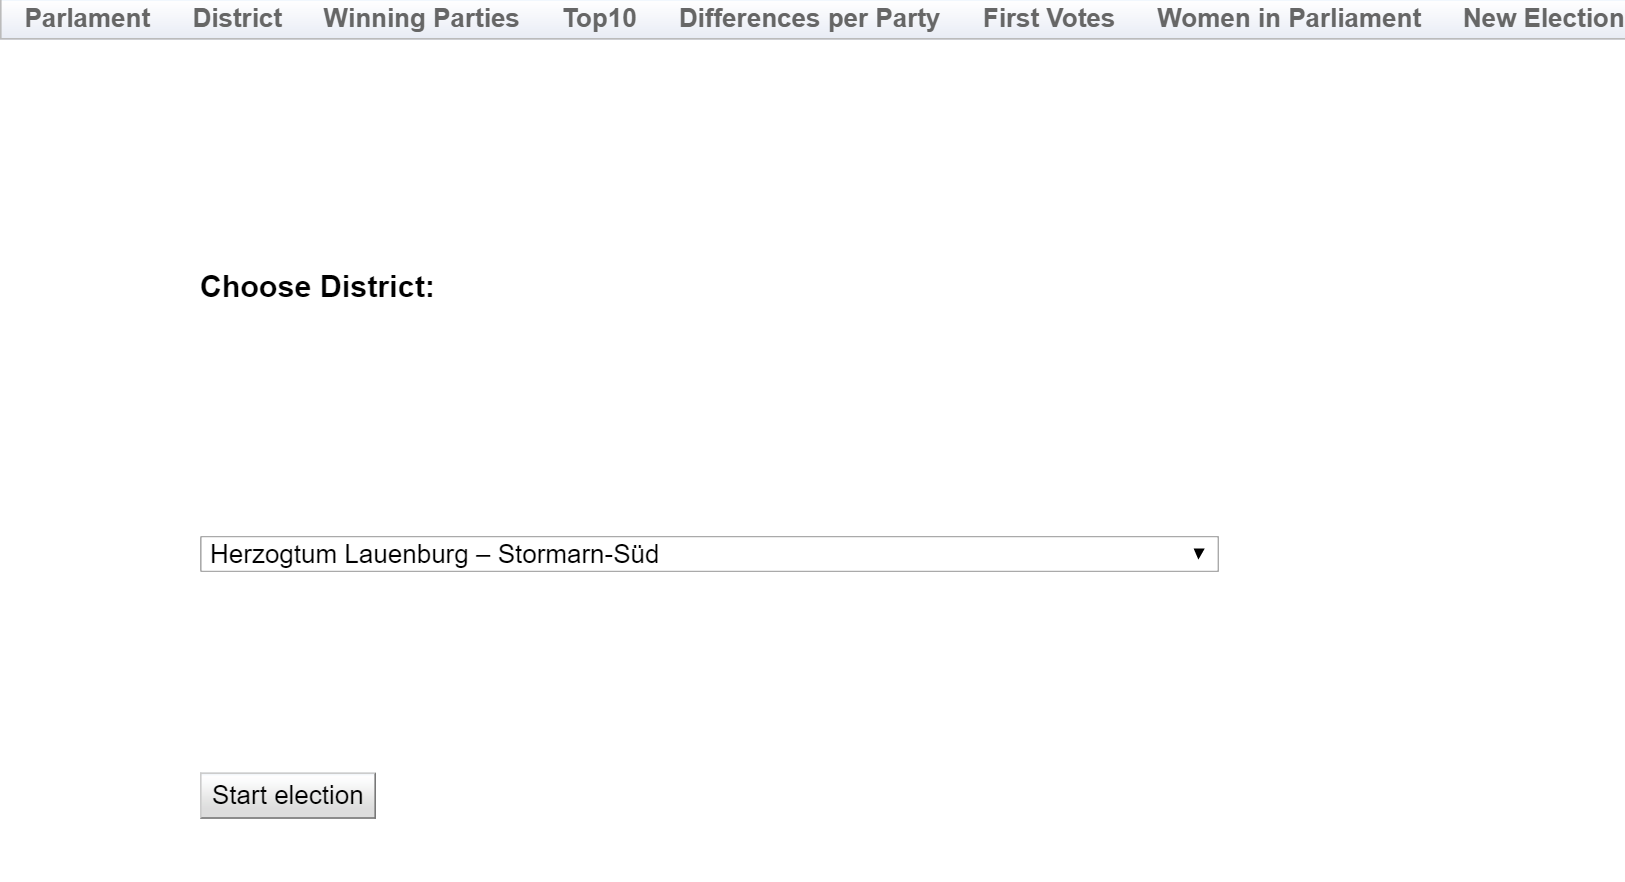
\includegraphics[width=\textwidth]{images/select_district.png}
\caption {District selection view}
\end{figure}

Nach Auswahl eines Wahlkreises wird eine Eingabemaske gezeigt, in der ein Wähler später ein Wahltoken eingeben kann. Nach Eingabe eines gültigen Tokens wird der Stimmzettel angezeigt, auf dem der Wähler wählen kann. Die wählbaren Direktkandidaten und Landeslisten werden dabei in der gleichen Reihenfolge angezeigt, die sie auch auf einem konventionellen Stimmzettel haben würden. Dabei orientiert sich die Reihenfolge der Parteien an der Anzahl der Zweitstimmen, die sie bei der vorherigen Bundestagswahl in dem entsprechenden Bundesland des Wahlkreises erhalten haben.

\begin{figure}[H]
\centering
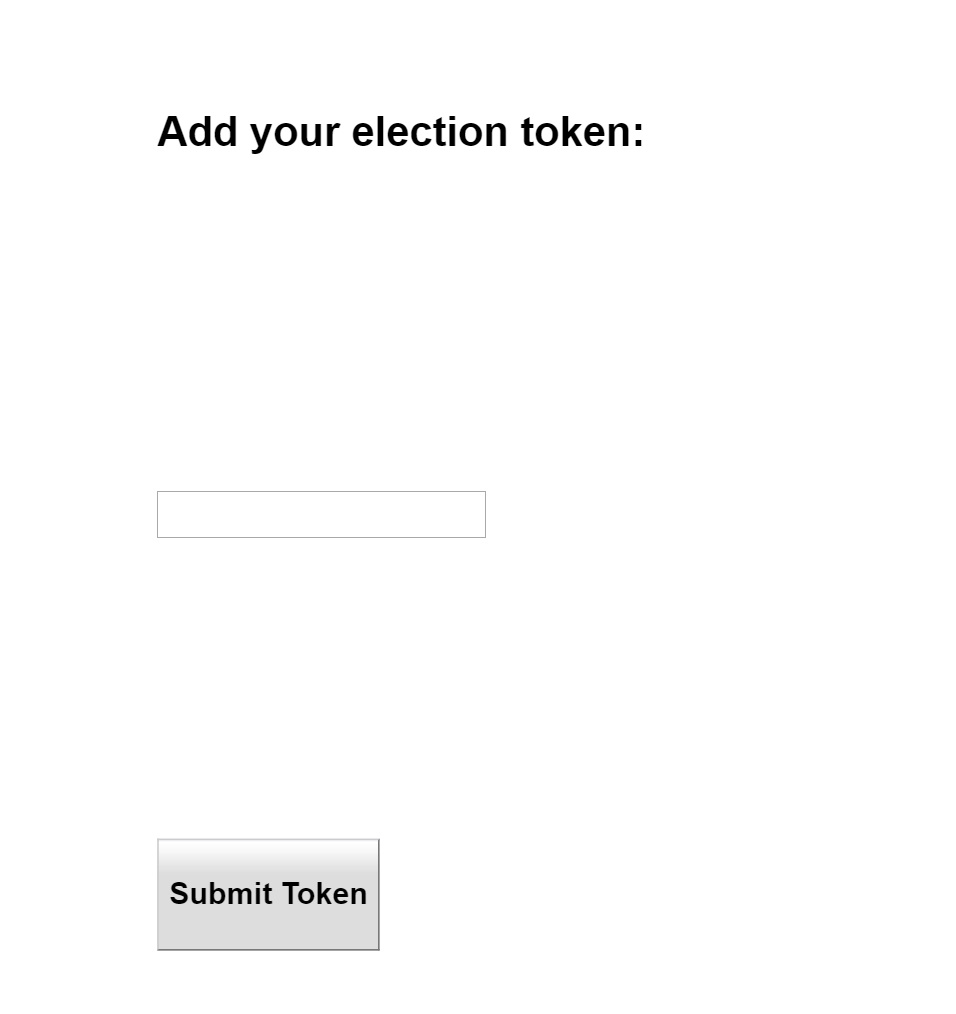
\includegraphics[width=\textwidth]{images/token_input.png}
\caption {Token input view}
\end{figure}

\begin{figure}[H]
\centering
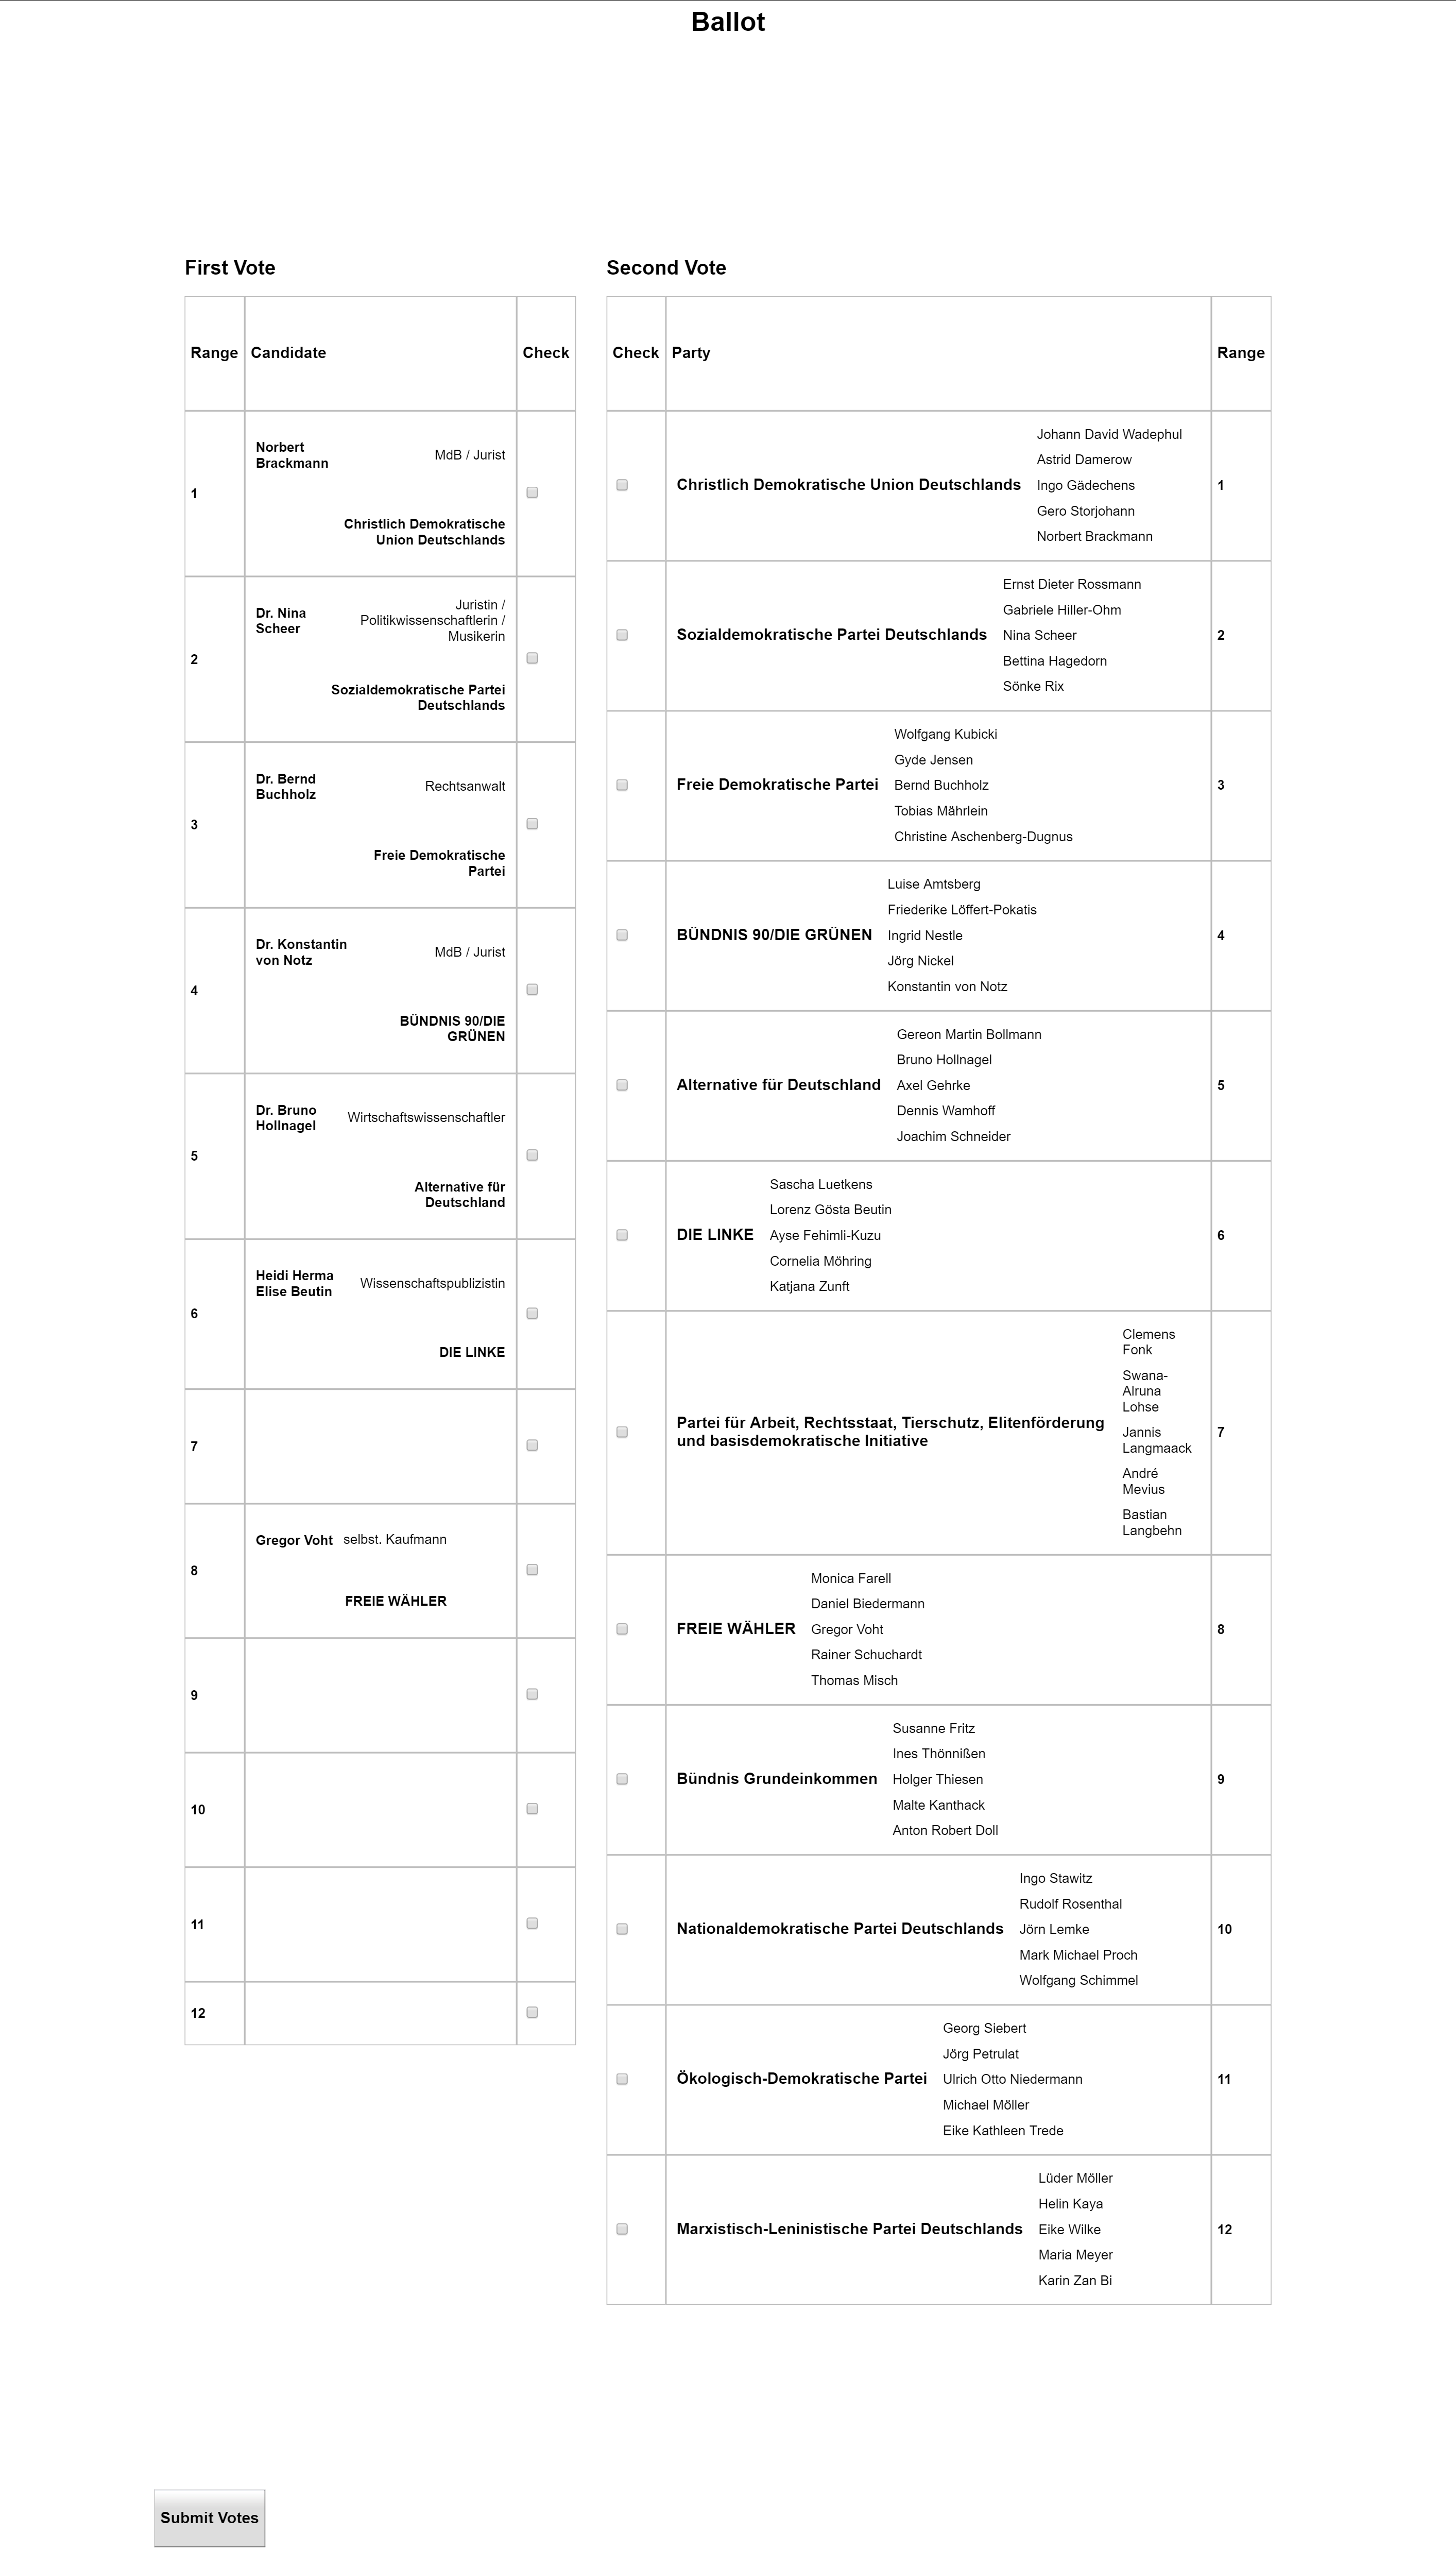
\includegraphics[width=0.8\textwidth]{images/ballot.png}
\caption {Ballot view}
\end{figure}

Aus Sicherheitsgründen muss die Website auf dem Wahlcomputer in den Vollbildmodus versetzt werden. Der Wähler darf keine Möglichkeit haben, diesen Vollbildmodus zu beenden. So kann sichergestellt werden, dass der Wähler ausschließlich die vorbereitete Eingabemaske benutzen kann.

\subsection{Wahl}

Ein Wähler kommt in das Wahllokal mit seinem Personalausweis und seiner Wahlberechtigung.
Die Wahlhelfer registrieren den Wähler konventionell.
Nun darf der Wähler ein Zettel mit einem Wahltoken nehmen.
Hierbei stellen die Wahlhelfer sicher, dass jeder Wähler genau ein Token nimmt.

Nun darf der Wähler zum Terminal gehen, sein Token in die Maske eintragen und seine Wahl abgeben. Dabei kann die Stimme manuell ungültig gemacht werden, indem etwa für die Erst- oder Zweitstimme eine leere Zeile oder gar keine Zeile ausgewählt wird.
Anschließend bestätigt der Wähler seine Eingabe. Nachdem der Wähler seine Stimme so abgegeben hat wird wieder die initiale Eingabemaske angezeigt, sodass der nächste Wähler wählen kann.

\subsection{Sicherheitskonzept}

\subsubsection{Tokens}

Damit die Tokens gegen Brute-Force Attacken geschützt sind, müssen die Tokens eine bestimmte Entropie aufweisen.
Hierbei gilt: Die Anzahl der \textit{möglichen} Tokens dividiert durch die Anzahl der \textit{benötigten} Tokens darf $2^{40}$ nicht unterschreiten.

Hierzu genügt aktuell (ca. 50 Millionen Wähler) beispielsweise ein alphanumerisches, case-insensitives Token mit 16 Zeichen (der Rest-Puffer wäre hierbei ca. 140, das heißt dass wir die Anzahl der Wähler noch um Faktor 140 vergrößern könnten, bevor das Token zu kurz wird).
Zusätzlich wird im System jeder Wahlversuch mit einem falschen Token geloggt, sodass Brute-Force Angriffe rückwirkend nachweisbar wären.

\subsubsection{Absicherung des Systems}

Zur weiteren Absicherung gegen Brute-Force-Attacken wird der öffentliche Zugriff auf das produktive Wahlsystem für die Dauer der Wahl entzogen. Die Wahlergebnisse dürfen ohnehin nicht vor dem Ende der Wahl veröffentlicht werden. Des Weiteren kann eine Kopie des Systems weiterhin öffentlich erreichbar sein. Das produktive Wahlsystem wird hierbei in einem privaten Netzwerk betrieben, wobei der Zugriff von den Wahlcomputern via VPN stattfindet.

\subsubsection{Absicherung des Wahlcomputers}

Die Weboberfläche auf jedem Wahlcomputer muss den Zugriff nach 10 konsekutiven Fehlversuchen für die Eingabe des Tokens sperren und kann nur durch einen Wahlhelfer, der den Vollbildmodus beenden und die Seite neu laden kann, wieder entsperrt werden.
So wird zusätzlich das zufällige Ausprobieren von Zeichenketten verhindert.

\section{Benchmarks}

Die Performance sowie die Ressourcenauslastung des Systems wurde mit Apache JMeter\footnote{\url{https://jmeter.apache.org/}} getestet.
Da das verwendete Framework, GWT, zwischen Frontend und Backend mit authentifizierten RPCs kommuniziert, haben wir separat ein REST-Interface programmiert.
Die durchgeführten Berechnungen im Backend sind dabei die selben wie beim Aufruf einer Seite des Frontends.

Die JMeter-Konfiguration, die dem Projekt beiliegt, sendet zufällige Anfragen an den Server.
Dabei ist die Parallelität, also die Anzahl der simulierten User, sowie die Verzögerung zwischen zwei Anfragen eines Users frei konfigurierbar.

Da uns zum Entwicklungszeitpunkt leider kein potenter Server zur Verfügung steht, können wir keine Hardwareempfehlungen für die Software geben.
Jedoch konnten wir in den Benchmarks feststellen, dass die Performance des Backends bei zusätzlichen Nutzern linear skaliert, bis alle Ressourcen des Servers aufgebraucht sind.
Dies bedeutet, dass sich die Anwendung mit entsprechenden Servern nahezu beliebig skalieren lässt.

Ein zusätzliches Caching der Anfragen könnte leicht in die Anwendung eingebaut werden und würde zu einer wesehtlich höheren Skalierbarkeit führen, da die Anwendung zusätzliche, parallele Anfragen dann in vernachlässigbarer Zeit durchführen könnte.

Die Ergebnisse der Benchmarks befinden sich im Anhang~\ref{apx:bench}.


\chapter{Lastenheft}

Im Folgenden werden die Anforderungen an das Wahlinformationssystem knapp zusammengefasst dargestellt.

\section{Benutzerschnittstellen}

Folgende Aktionen sollen für einen Nutzer des Wahlinformationssystems möglich sein: 

\begin{itemize}
\item Abfrage des Ergebnisses der Bundestagswahl von 2013 oder 2017, bestehend aus der Sitzverteilung im Bundestag, der Überhangmandate und der Mitglieder des Bundestags
\item Abfrage der Ergebnisse der Bundestagswahl eines beliebigen Wahlkreises, bestehend aus der Wahlbeteiligung, des gewählten Direktkandidaten, der Anzahl an Erst- und Zweitstimmen und die für jede Partei abgegeben wurden. Die Entwicklung der Verteilung der Stimmen im Vergleich zum Vorjahr soll hier sichtbar sein. 
\item Abfrage einer Auflistung aller Wahlkreise und der Parteien, die in diesem Wahlkreis die meisten Erst- oder Zweitstimmen erhalten haben. 
\item Die Abfrage der Kandidaten einer Partei, die in ihrem Wahlkreis besonders knapp gewonnen oder verloren haben.
\end{itemize}

\section{Funktionale Anforderungen}

\subsection{Ui-Anf-1}

Das System muss dem Nutzer die Möglichkeit bieten verschiedene Wahljahre auszuwählen. Alle Abfragen müssen für die Bundestagswahlen von 2017 und, soweit entsprechende Daten zur Verfügung stehen, 2013 möglich sein. 

\subsection{Ui-Anf-3}

Das System muss dem Nutzer eine Übersicht der gesamten Wahldaten in aufbereiteter Form einzusehen. Die Wahldaten  müssen in Form von Charts und Diagrammen visualisiert und verständlich dargestellt werden. Ein unbeteiligter Nutzer muss in der Lage sein, die Sicht ohne zusätzliche Anleitungen zu verstehen.

\subsection{Ui-Anf-4}

Das System muss dem Nutzer die Möglichkeit bieten die Ergebnisse einer Wahl für einen bestimmten Wahlkreis anzuzeigen. 

\subsection{Ui-Anf-5}

Die Applikation muss in einem Browser ausgeführt werden können. Durch Eingabe einer URL im Browser muss sich die Applikation öffnen und nutzbar sein.

\subsection{Backend-Anf-1}

Das System muss eingetragene Daten auch nach Neustart noch laden können. Nach dem Neustart der Software muss das selbe Wahlergebnis zu den jeweiligen Wahlen sichtbar sein wie vor dem Neustart. 

\subsection{Backend-Anf-2}

Das System muss die Berechnung der Wahlergebnisse unter Berücksichtigung von bestimmten Sonderklauseln, wie etwa der 5-Prozent Hürde durchführen können. In der Gesamtübersicht der Stimmenverteilung werden Randparteien unter einem aggregierten Punkt dargestellt.  

\subsection{Backend-Anf-3}

Das System muss anhand der eingetragenen Stimmen nach dem aktuellen Wahlverfahren die Sitzverteilung des Bundestags berechnen können.

\subsection{Backend-Anf-4}

Das System soll die Wahlbeteiligung für einen ausgewählten Wahlkreis anzeigen.

\subsection{Backend-Anf-5}

Das System muss die Wahldaten in einer Datenbank persistieren.

\subsection{Backend-Anf-6}

Das System muss Überhangmandate in der Berechnung der Sitzverteilung im Bundestag mit einbeziehen und darstellen können.

\section{Nicht Funktionale Anforderungen}

\subsection{QM-Sicherheit}

Das System muss den heutigen Sicherheitsstandards entsprechen. Die Stimmen dürfen nur anonymisiert abgespeichert werden. Stimmdaten dürfen nicht mit persönlichen Daten eines Wählers in Verbindung gebracht werden können.

\subsection{QM-Robustheit}

Das System arbeitet auch unter sehr hoher Last fehlerfrei. Eine sehr hohe Anzahl von Anfragen darf die Daten des Systems in keiner Weise beeinflussen. Der Nutzer soll weiterhin nur eine vertretbare Wartezeit haben.

\subsection{QM-Wiederherstellbarkeit}

Das System muss nach einem Neustart den selben validen Zustand wie zuvor haben. Die angezeigten Daten dürfen sich nach einem Neustart nicht verändert haben.

\subsection{QM-Erlernbarkeit}

Der Nutzer muss die Applikation ohne Zuhilfenahme einer Dokumentation verstehen. Ein Unbeteiligter muss nach 15 Minuten fähig sein mit der Software umzugehen.

\subsection{QM-Einfachheit}

Die Benutzerschnittstellen sollen möglichst einfach gestaltet werden und keine überflüssigen Informationen beinhalten. Die Sichten der Applikation sollen nicht überladen wirken, aber trotzdem alle wichtigen Informationen beinhalten.

\subsection{RG-1}

Die Software wird in der Programmiersprache Java verfasst, nutzt zur Oberflächengenerierung GWT und arbeitet mit einer PostgreSQL Datenbank zusammen.
 
 

\chapter{Pflichtenheft}

In diesem Projekt soll ein Wahlinformationssystem entwickelt werden. Das System soll einem Nutzer die Ergebnisse der aktuellen oder einer vorherigen Bundestagswahl anzeigen können. Der Nutzer soll sich mit Hilfe des Systems unter anderem über die Stimmenverteilung einer Wahl informieren können. Diese Daten sollen nicht nur für die gesamte Wahl, sondern auch auf Wahlkreisebene angezeigt werden können. Das System soll für die elektronische Abgabe von Stimmen genutzt werden können. 

\section{Zielbestimmung}

Im Folgenden werden die Ziele des zu entwickelten Systems dargestellt. Auch einige nicht notwendige Funktionen werden vorgestellt.
 
\subsection{Musskriterien}

Das System muss dem Nutzer eine Übersicht der gesamten Wahlergebnisse der aktuellen oder einer vorherigen Bundestagswahl in aufbereiteter Form geben. Die Wahldaten müssen dabei in einer Datenbank persistent abgelegt werden. Anhand der in dieser Datenbank abgelegten Stimmen muss das System die Sitzverteilung des Bundestags nach dem aktuellen Wahlverfahren berechnen können. Dabei müssen Sonderklauseln wie die 5-Prozent-Hürde berücksichtigt werden. Auch Überhangmandate müssen korrekt berechnet werden können. Um eine möglichst schnelle Anzeige der Wahlergebnisse zu ermöglichen sollen Wahlergebnisse in der Datenbank voraggregiert werden können. Die Ergebnisse einer Bundestagswahl müssen auch auf Wahlkreisebene angezeigt werden können. Auf Wahlkreisebene muss angezeigt werden, wie viele Stimmen die einzelnen Landeslisten der Parteien erhalten haben. Zudem muss die Stimmverteilung unter den Direktkandidaten angezeigt werden. 

\subsection{Sollkriterien}

Das System soll dem Nutzer die Möglichkeit bieten, elektronisch eine Stimme abzugeben. Diese Stimmabgabe soll in einem Wahllokal mit einem dort ausgegebenen Code erfolgen. Es sollen nur Stimmen für Direktkandidaten oder Landeslisten abgegeben werden können, die in dem Wahlkreis, in dem die Stimme abgegeben wird, auch antreten. Auch die Abgabe von ungültigen Stimmen soll möglich sein. Aus Datenschutzgründen sollen abgegebene Stimmen nur anonymisiert gespeichert werden. Eingetragene Stimmen sollen auch in der Datenbank abgelegt werden und auch nach Neustart des Systems noch zur Verfügung stehen. Sie sollen auch bei der Berechnung des Wahlergebnisses berücksichtigt werden. 

\subsection{Kannkriterien}

Das System soll dem Nutzer die Möglichkeit bieten, sich die Wahlbeteiligung einer Bundestagswahl in einem Wahlkreis anzeigen zu lassen. Hier soll das System die Anzahl der Wähler im Vergleich zur Anzahl der Wahlberechtigten in dem Wahlkreis anzeigen können. 
 
\subsection{Abgrenzungskriterien}

Das System muss die Ergebnisse von Bundestagswahlen vor 2013 nicht anzeigen können. Zudem müssen Wahlergebnisse nur nach dem aktuellen Verfahren berechnet werden können. Eine Berechnung nach anderen Verfahren, etwa zum Vergleich der Verteilung der Überhangmandate bei verschiedenen Verfahren, wird nicht benötigt. Das System muss keine Ergebnisse für die Bundestagswahl 2013 anzeigen können, die sich auf Kandidatendaten beziehen. Zu diesen Ergebnissen gehört etwa die prozentuale Anzahl der Frauen im Bundestag.
 
\section{Einsatz}
Das System ist für den Einsatz als Informationssystem gedacht. Über eine Webseite soll sich der Nutzer über die Ergebnisse der aktuellen oder einer vorherigen Bundestagswahl informieren können. Zudem soll das System für die elektronische Stimmabgabe eingesetzt werden können, indem es einem Nutzer die Möglichkeit bietet, eine Stimme mit einem in einem Wahllokal ausgeteilten Code abzugeben.
 
\subsection{Anwendungsbereiche}
Angewendet wird das System von Nutzern, die sich über die Ergebnisse einer Bundestagswahl informieren wollen. Zudem soll das System in Wahllokalen für die elektronische Abgabe von Einzelstimmen genutzt werden können.
 
\subsection{Zielgruppen}
Die Zielgruppe umfasst Bürger, die sich für das Ergebnis einer Bundestagswahl interessieren. Die Zielgruppe für die elektronische Abgabe von Einzelstimmen sind Bürger, die ihre Stimme in einem Wahllokal elektronisch abgeben wollen. 

\section{Umgebung}
Die Software wird in der Programmiersprache Java verfasst. Sie nutzt zur Oberflächengenerierung GWT und arbeitet mit einer PostgreSQL Datenbank.
 
\subsection{Software}
Zum Betrieb des Servers muss mindestens Docker installiert sein.
Das gleiche gilt für den Betrieb der Datenbank.
Um die Anwendung benutzen zu können ist Webbrowser nötig.
Unterstützt wird der Google Chrome Browser.
 
\subsection{Hardware}
Die Systemhardware muss der Benutzerzahl angepasst werden.
Die Funktionalität des Systems für geringe Benutzerzahlen kann mit 8 GB freiem RAM, 30 GB freiem Festplattenspeicher und einer Intel CPU vom Typ Core i5-6000 oder besser gewährleistet werden.
 

\section{Funktionalität}
Im folgenden werden einzelne Funktionen des Systems näher vorgestellt. 
 
\subsection{Anzeige des Wahlergebnisses einer Bundestagswahl}
\begin{itemize}
\item Primärer Akteur: Bürger
\item Trigger: Bürger möchte Informationen über Ergebnisse einer Bundestagswahl
\item Haupterfolgsszenario:
\begin{enumerate}
\item Nutzer wählt die Option "Parlament"
\item System berechnet anhand von voraggregierten Wahlergebnissen Ergebnis der Bundestagswahl
\item System zeigt Wahlergebnis bestehend aus prozentualer und absoluter Verteilung von Stimmen auf Parteien, Sitzverteilung im Bundestag, Anzahl der Überhangmandate und Mitglieder des Bundestages an
\end{enumerate}
\item Alternative Szenarien:
\begin{enumerate}
\item a) Nutzer möchte sich die Ergebnisse einer vorherigen Bundestagswahl anzeigen lassen und wählt deshalb statt dem voreingestellten Jahr der letzten Bundestagswahl ein vorheriges 
\end{enumerate}
\item Oberfläche Beispiel: \\
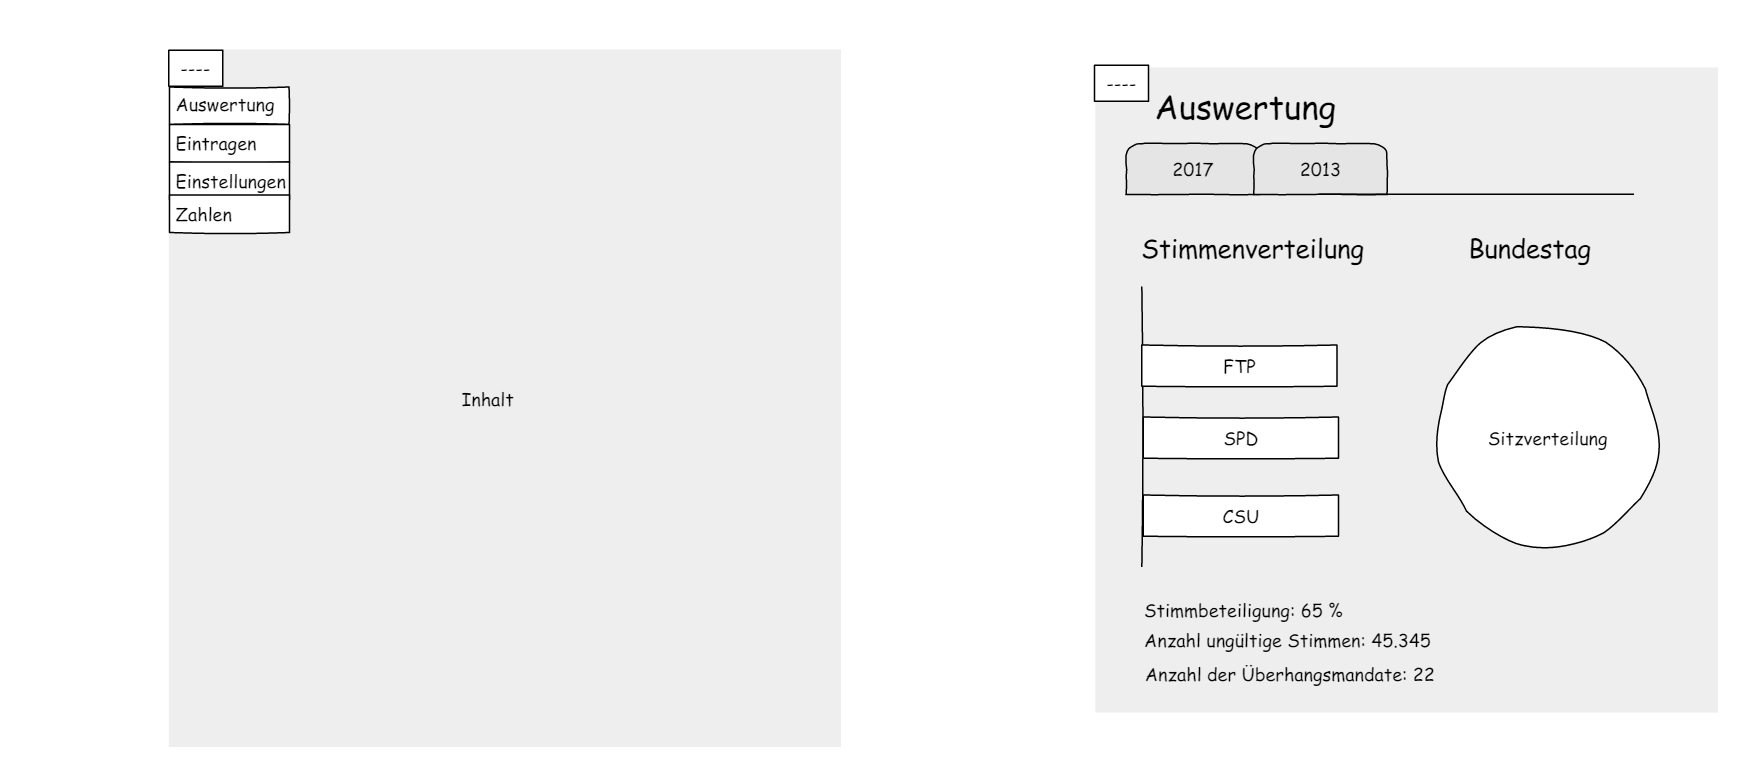
\includegraphics[width=.9\textwidth]{images/gesamt.png}
\end{itemize}

\subsection{Anzeige des Wahlergebnisses einer Bundestagswahl in einem Wahlkreis}
\begin{itemize}
\item Primärer Akteur: Bürger
\item Trigger: Nutzer möchte sich über die Ergebnisse einer Bundestagswahl in einem Wahlkreis informieren
\item Haupterfolgsszenario:
\begin{enumerate}
\item Nutzer wählt die Option "District"
\item Nutzer wählt Wahlkreis aus einer Vorschlagsliste
\item System zeigt Wahlergebnis des Wahlkreises bestehend aus prozentualer und absoluter Verteilung von Stimmen auf Landeslisten und Direktkandidaten und die Anzahl der Wähler und Nichtwähler. Diese Daten werden im Vergleich zu den Daten der vorherigen Bundestagswahl dargestellt.
\end{enumerate}
\item Oberfläche Beispiel: \\
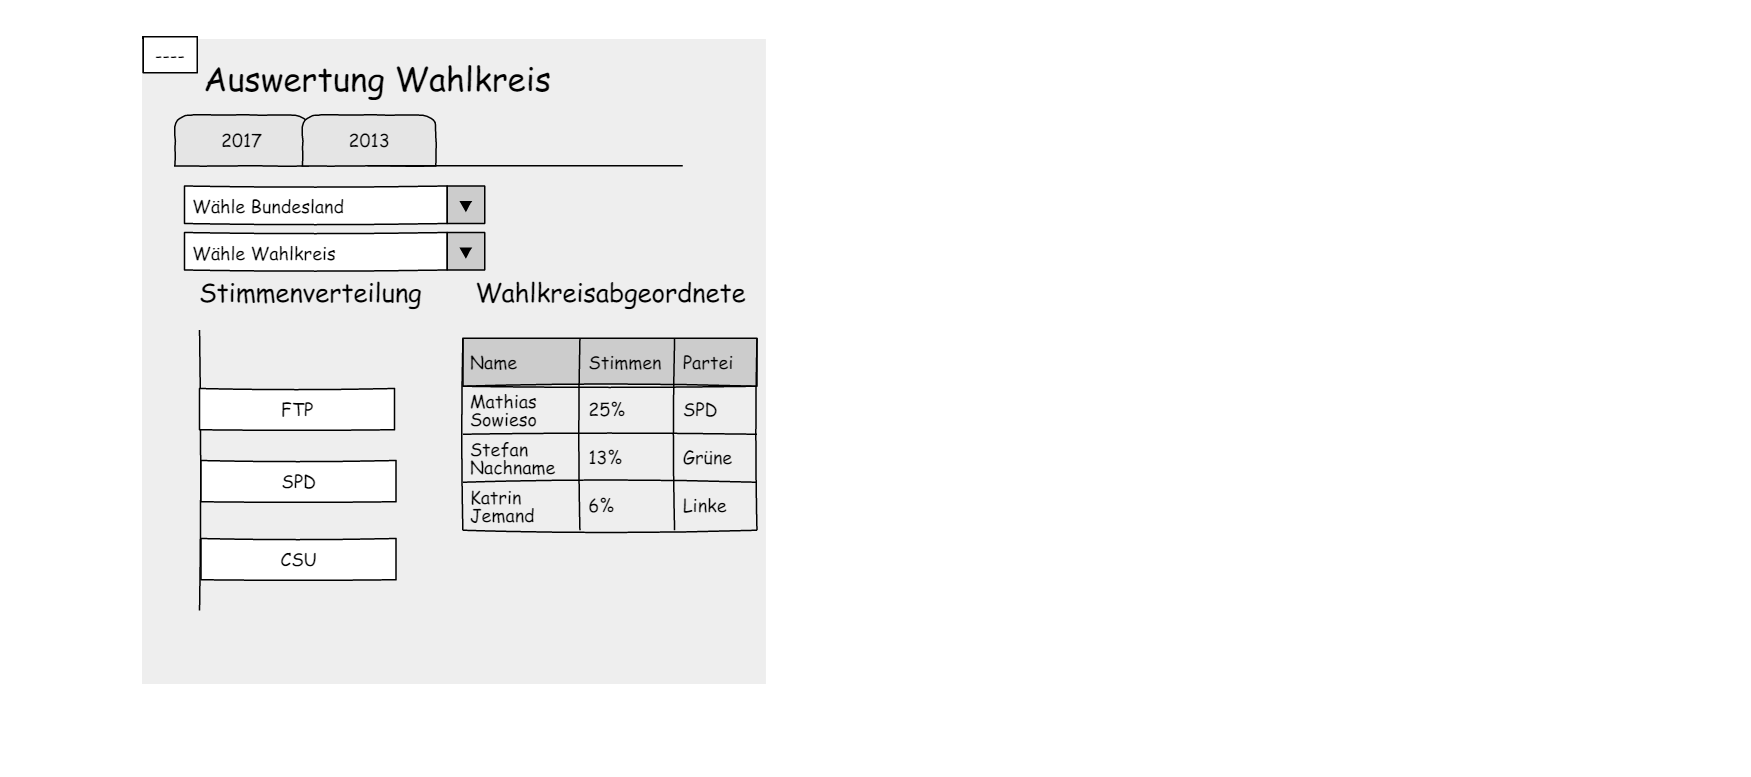
\includegraphics[width=.9\textwidth]{images/wahlkreis.png}
\end{itemize}

\subsection{Abgabe einer Einzelstimme}
\begin{itemize}
\item Primärer Akteur: Wähler
\item Trigger: Nutzer möchte bei einer Bundestagswahl seine Stimme in elektronischer Form abgeben
\item Vorbedingung: Das System zeigt ein Eingabefeld für einen Autorisierungscode für die elektronische Stimmabgabe an
\item Haupterfolgsszenario:
\begin{enumerate}
\item Nutzer gibt Authentifizierungscode an
\item System prüft Code
\item System zeigt Stimmzettel mit wählbaren Direktkandidaten und Landeslisten an
\item Nutzer vergibt Erststimme an einen Direktkandidaten
\item Nutzer vergibt Zweitstimme an eine Landesliste
\end{enumerate}
\item Alternative Szenarien:
\begin{itemize}
\item Nutzer möchte Erst- oder Zweitstimme nicht an einen Kandidaten oder eine Landesliste vergeben
\begin{itemize}
\item Nutzer wählt keinen Kandidaten oder keine Landesliste
\end{itemize}
\item Authentifizierungscode ist ungültig
\begin{itemize}
\item System informiert Nutzer entsprechend und fordert ihn zur erneuten Eingabe des Codes auf
\end{itemize}
\end{itemize}
\item Oberfläche Beispiel: \\
i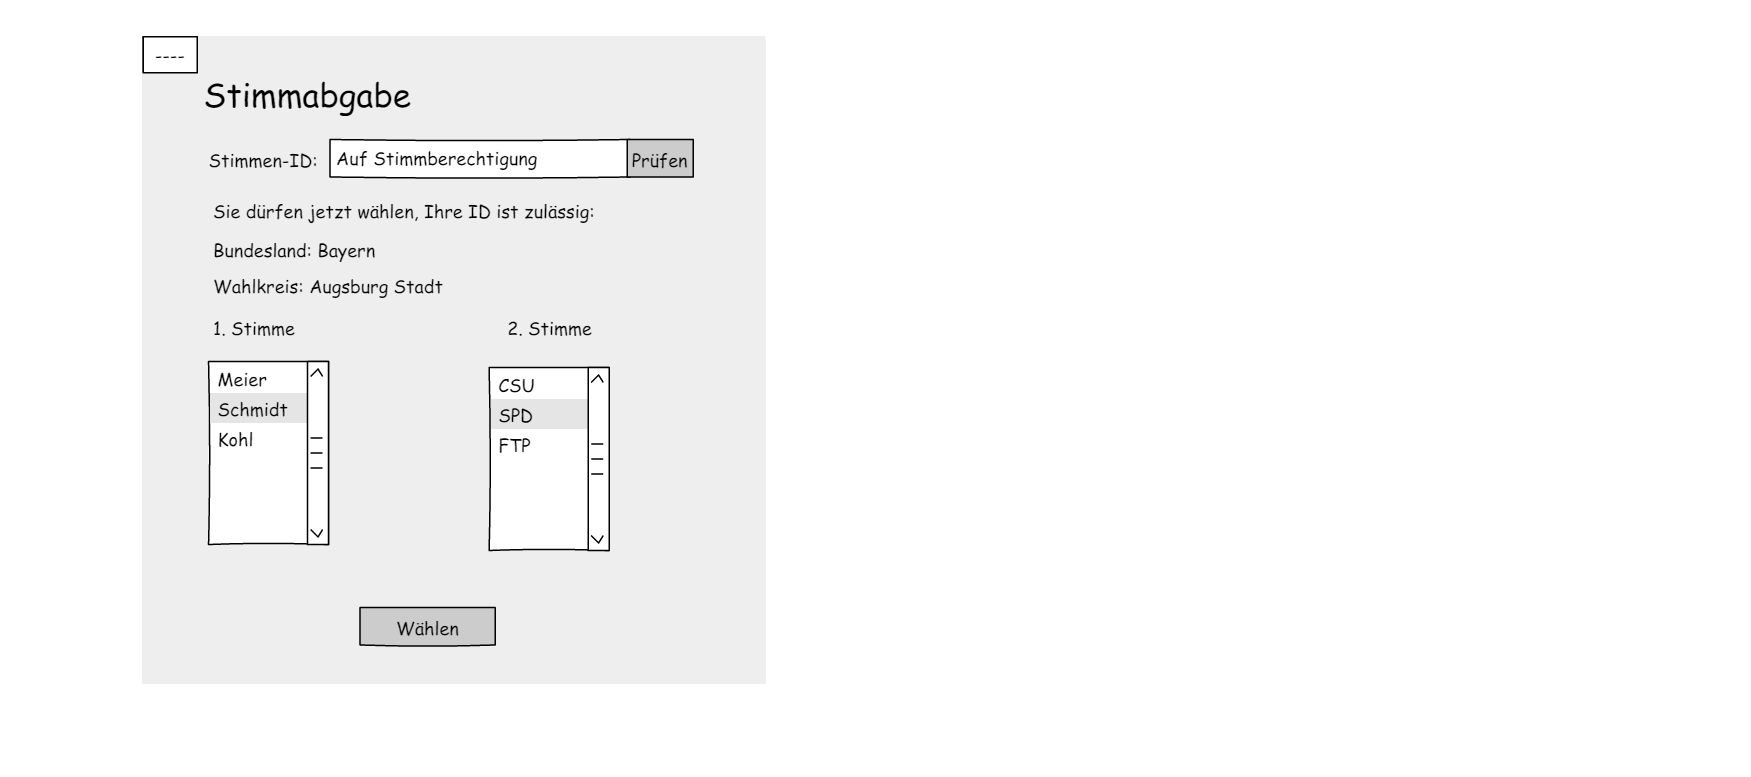
\includegraphics[width=.9\textwidth]{images/whlen.png}
\end{itemize}
 
\subsection{Nichtfunktionale Anforderungen}
Im Folgenden sind die nichtfunktionalen Anforderungen spezifiziert:

\subsection{Sicherheit}
Um die Sicherheit zu gewährleisten muss der Betreiber des Systems folgendes beachten:
\begin{itemize}
  \item Die Datenbank darf in Produktivsystemen nur aus einem abgeschotteten Netz zugreifbar sein.
  	In diesem darf sich außer der Datenbank nur der Server befinden.
    \begin{itemize}
    	\item Wenn nötig, darf ein autorisierter Techniker Wartungsarbeiten im Netz vornehmen, allerdings muss der Betreiber geeignete Maßnahmen ergreifen, um Datenintegrität und den Datenschutz gegenüber diesem sicherzustellen.
    \end{itemize}
  \item Die Eingabe sensibler Daten darf nur in einer gesicherten Umgebung möglich sein.
  	Verschiedene Möglichkeiten zur Umsetzung durch den Betreiber sind denkbar:
    \begin{itemize}
      \item Verwenden in einem abgeschotteten Netz
      \item Sicherung mittels aktueller Verschlüsselungstechnik und PFS\footnote{Perfect Forward Secrecy}, zum Beispiel mittels TLS\footnote{Transport Layer Security}
    \end{itemize}
\end{itemize}

\subsubsection{Datenschutz}
Der Datenschutz ist gewährleistet, da die Anwendung sensible Daten (insbesondere einzelne Stimmen) nur in akkumulierter Form an den Nutzer weiter gibt.

\subsubsection{Manipulationssicherheit}
Die Daten können nur durch Stimmenabgabe und direkte Manipulation an der Datenbank manipuliert werden.
Letzteres muss vom Betreiber ausgeschlossen werden.
Um ersteres zu gewährleisten, muss der Betreiber zur Stimmenabgabe einen unkompromittierten Kommunikationsweg sicherstellen.

Die Abgabe einer einzelnen Stimme direkt im Wahlbüro wird mit einem Sicherheitscode autorisiert, sodass nur autorisierte Personen die Stimmenabgabe durchführen können.
Ein Sicherheitscode berechtigt \textit{einmalig} zur Stimmenabgabe.
Ein Sicherheitscode ist entweder für eine Einzelstimme oder für die akkumulierte Stimmabgabe gültig, nie jedoch für beides.
Ein Sicherheitscode ist ausreichend lang, um Brute-Force Attacken auf aktueller Hardware (Stand Oktober 2017) zu verhindern.

\subsection{Robustheit und Verfügbarkeit}
Das System garantiert eine Uptime von 90\%, akkumuliert auf ein Jahr, sofern die Systemumgebung zur Verfügung steht.
Bei illegalen Eingaben in der Benutzerschnittstelle garantiert das System eine Robustheit.

\subsection{Korrektheit}
Die Analysen des Systems sind nach abgeschlossener Wahl bis auf die dritte signifikante Stelle korrekt.
Sollte die dritte signifikante Stelle einer Zahl von weniger als 10 Einzelstimmen abhängen, kann die Korrektheit der Analyse nicht garantiert werden.
 
\subsection{Nutzbarkeit}
Der Nutzer muss die Applikation ohne Zuhilfenahme einer Dokumentation verstehen. Auch ohne technische Vorkenntnisse soll er nach 15 Minuten fähig sein mit der Software umzugehen. Da die elektronische Abgabe von Einzelstimmen in Wahllokalen erfolgt soll hierfür keine Einarbeitungszeit nötig sein. Der Nutzer sollte für Authentifizierung und Stimmabgabe nicht länger als 5 Minuten brauchen. 

\subsection{Datengenerator}

Um die Funktionalität des Systems nachzuweisen soll ein Datengenerator implementiert werden. Dieser Generator soll die Erstellung von Stimmen, bestehend aus Erst- und Zweitstimme, ermöglichen, die den Stimmen letzten Bundestagswahl entsprechen. Aufgrund dieser Stimmen soll das korrekte Wahlergebnis berechnet werden können. 

\section{Daten}
Die Daten, die das System langfristig speichern soll können dem abgebildeten Datenmodell entnommen werden.

\noindent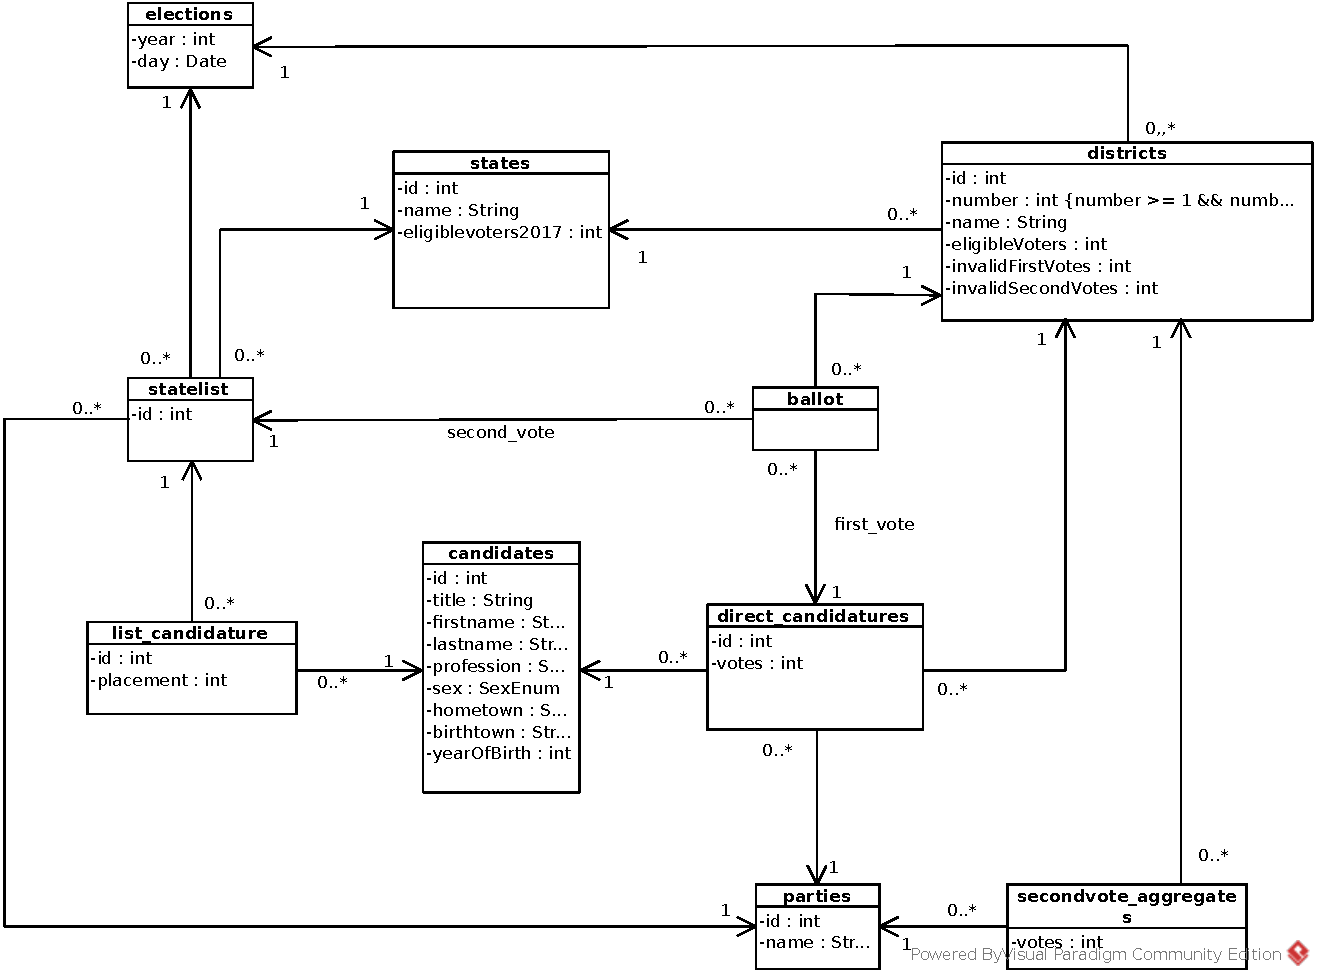
\includegraphics[width=\textwidth]{images/DBS_Schema.pdf}




\appendix
\chapter{Benchmark-Ergebnisse}\label{apx:bench}

\section{Methodik}

Die folgenden Benchmarks wurden auf einem Intel i5-3570K (3,4 GHz) System mit 16 Gigabyte RAM unter Linux ausgeführt.
Dabei lief jMeter zusammen mit der Anwendung sowie der Datenbank auf dem gleichen System.
Von den zur Verfügung stehenden 16 Gigabyte wurden während der Tests -- inklusive Betriebssystem -- nur ca. 3 Gigabyte genutzt.

Jeder durchgeführte Benchmark-Lauf hat 1 Minute lang mit mehreren simulierten Clients zufällig verteilte Anfragen für die Queries Q1 bis Q6 an den Server geschickt.
Jeder simulierte Client hat nach jeder Anfrage eine variable Zeitspanne gewartet, bevor er die nächste Anfrage gestartet hat.
Diese variable Zeitspanne ist zufällig gewählt aus einer Basiszeitspanne und dem 1.5-fachen dieser Basiszeitspanne.
Es wurden Benchmark-Läufe mit jeder Kombination aus 4, 20, 100 und 500 simulierten Clients sowie einer Basiszeitspanne von 1, 2, 4 und 8 Sekunden durchgeführt.
Jedes der folgenden Diagramme zeigt Boxplots, in welchen die Antwortzeiten für eine Query und eine Basiszeitspanne nach der Anzahl der simulierten Clients dargestellt sind.

Die jMeter-Konfiguration für die Benchmarks findet sich im Repository, damit können die Benchmarks leicht auf einem beliebigen System durchgeführt werden.

\begin{figure}[htb!]
	\centering
	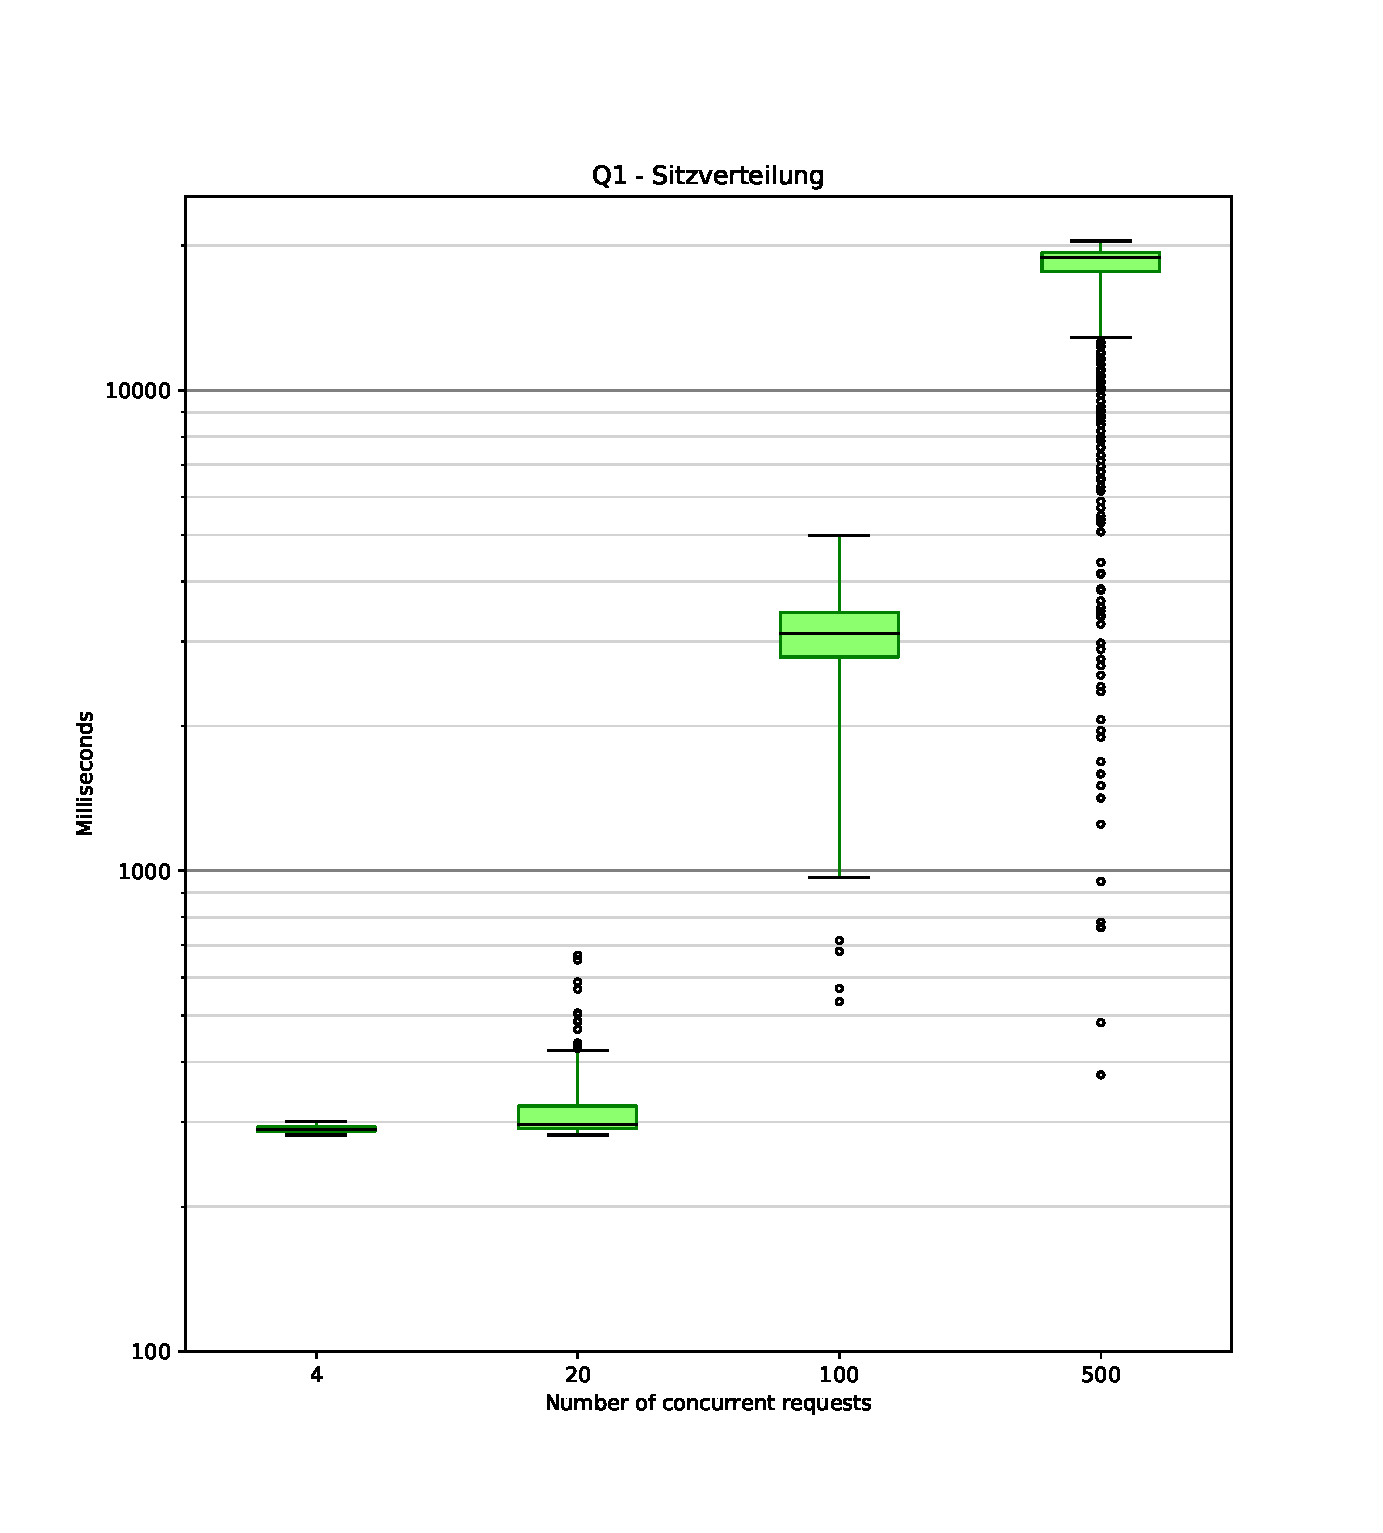
\includegraphics[width=0.9\textwidth]{images/plots_1s/Q1}
	\caption {Q1 - Sitzverteilung (1s)}
\end{figure}

\begin{figure}[htb!]
	\centering
	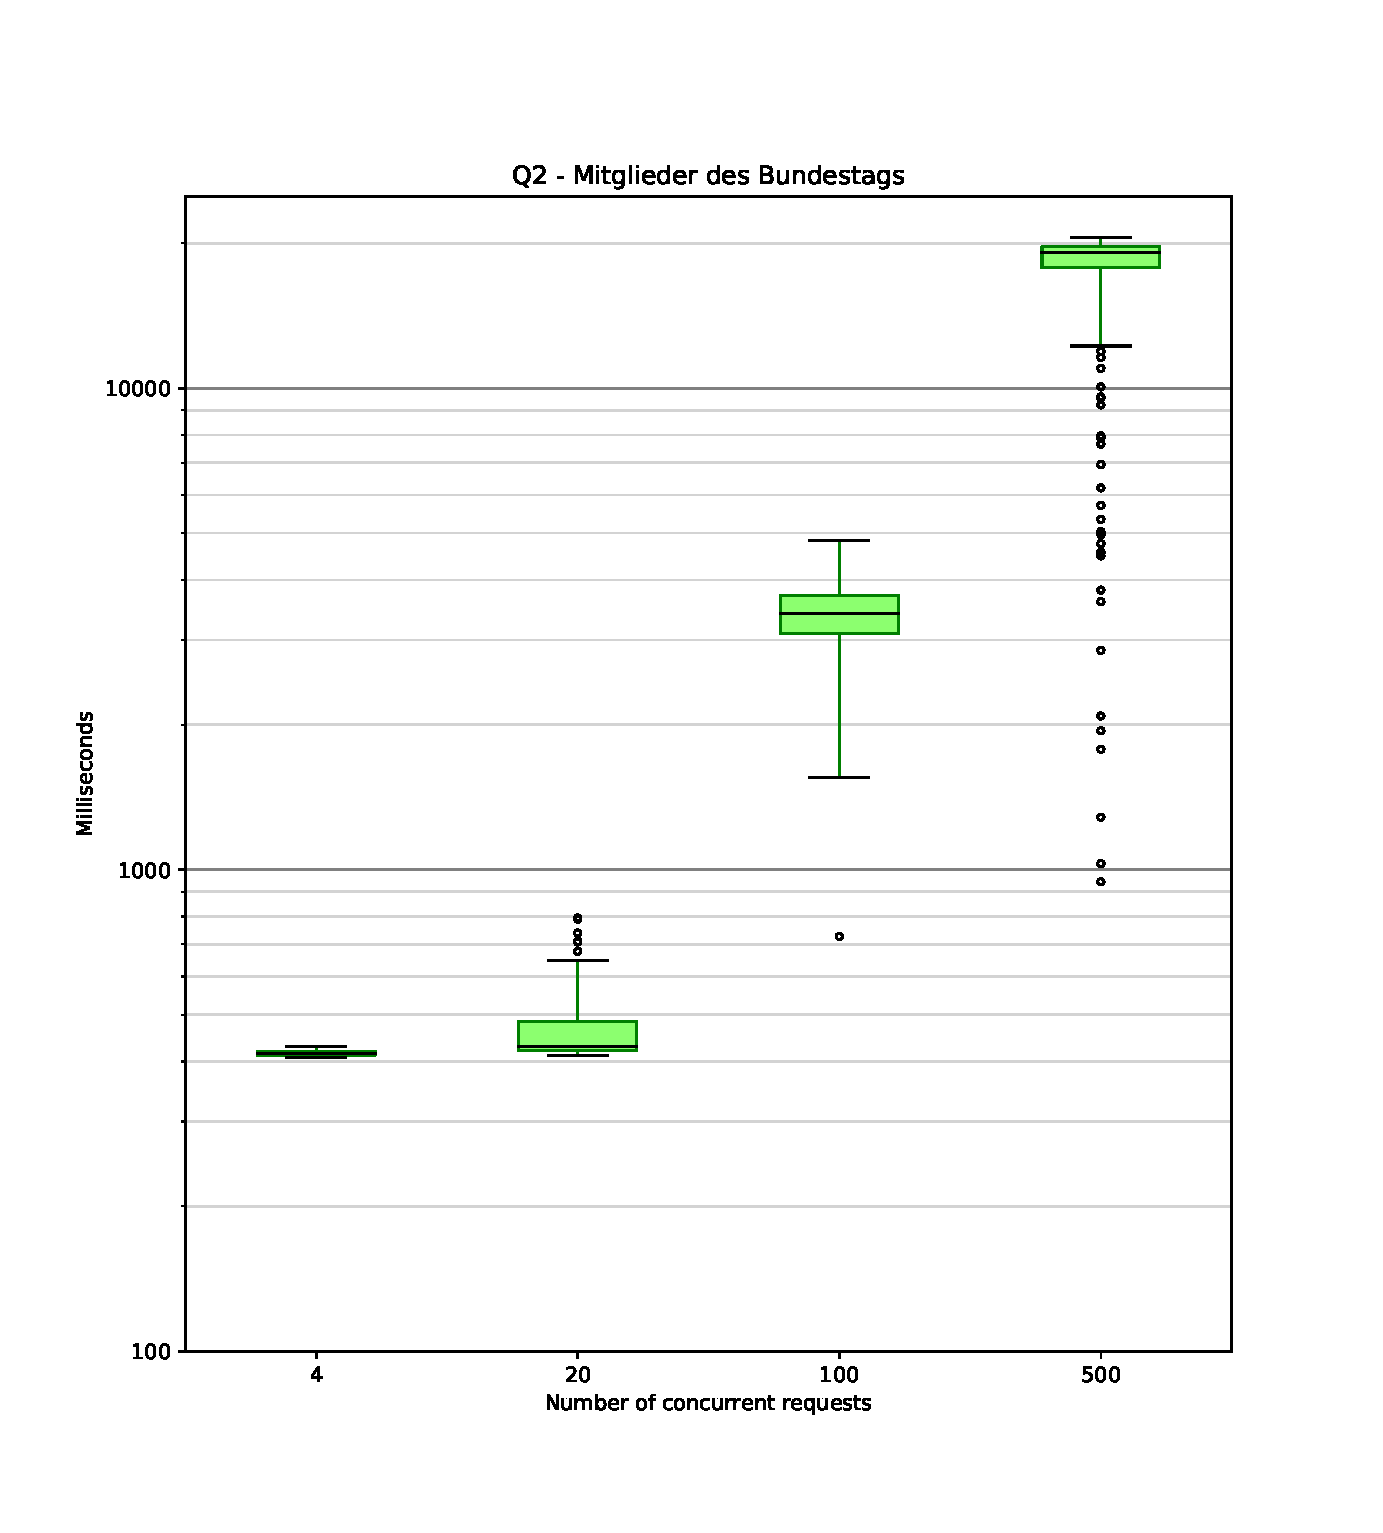
\includegraphics[width=0.9\textwidth]{images/plots_1s/Q2}
	\caption {Q2 - Mitglieder des Bundestags (1s)}
\end{figure}

\begin{figure}[htb!]
	\centering
	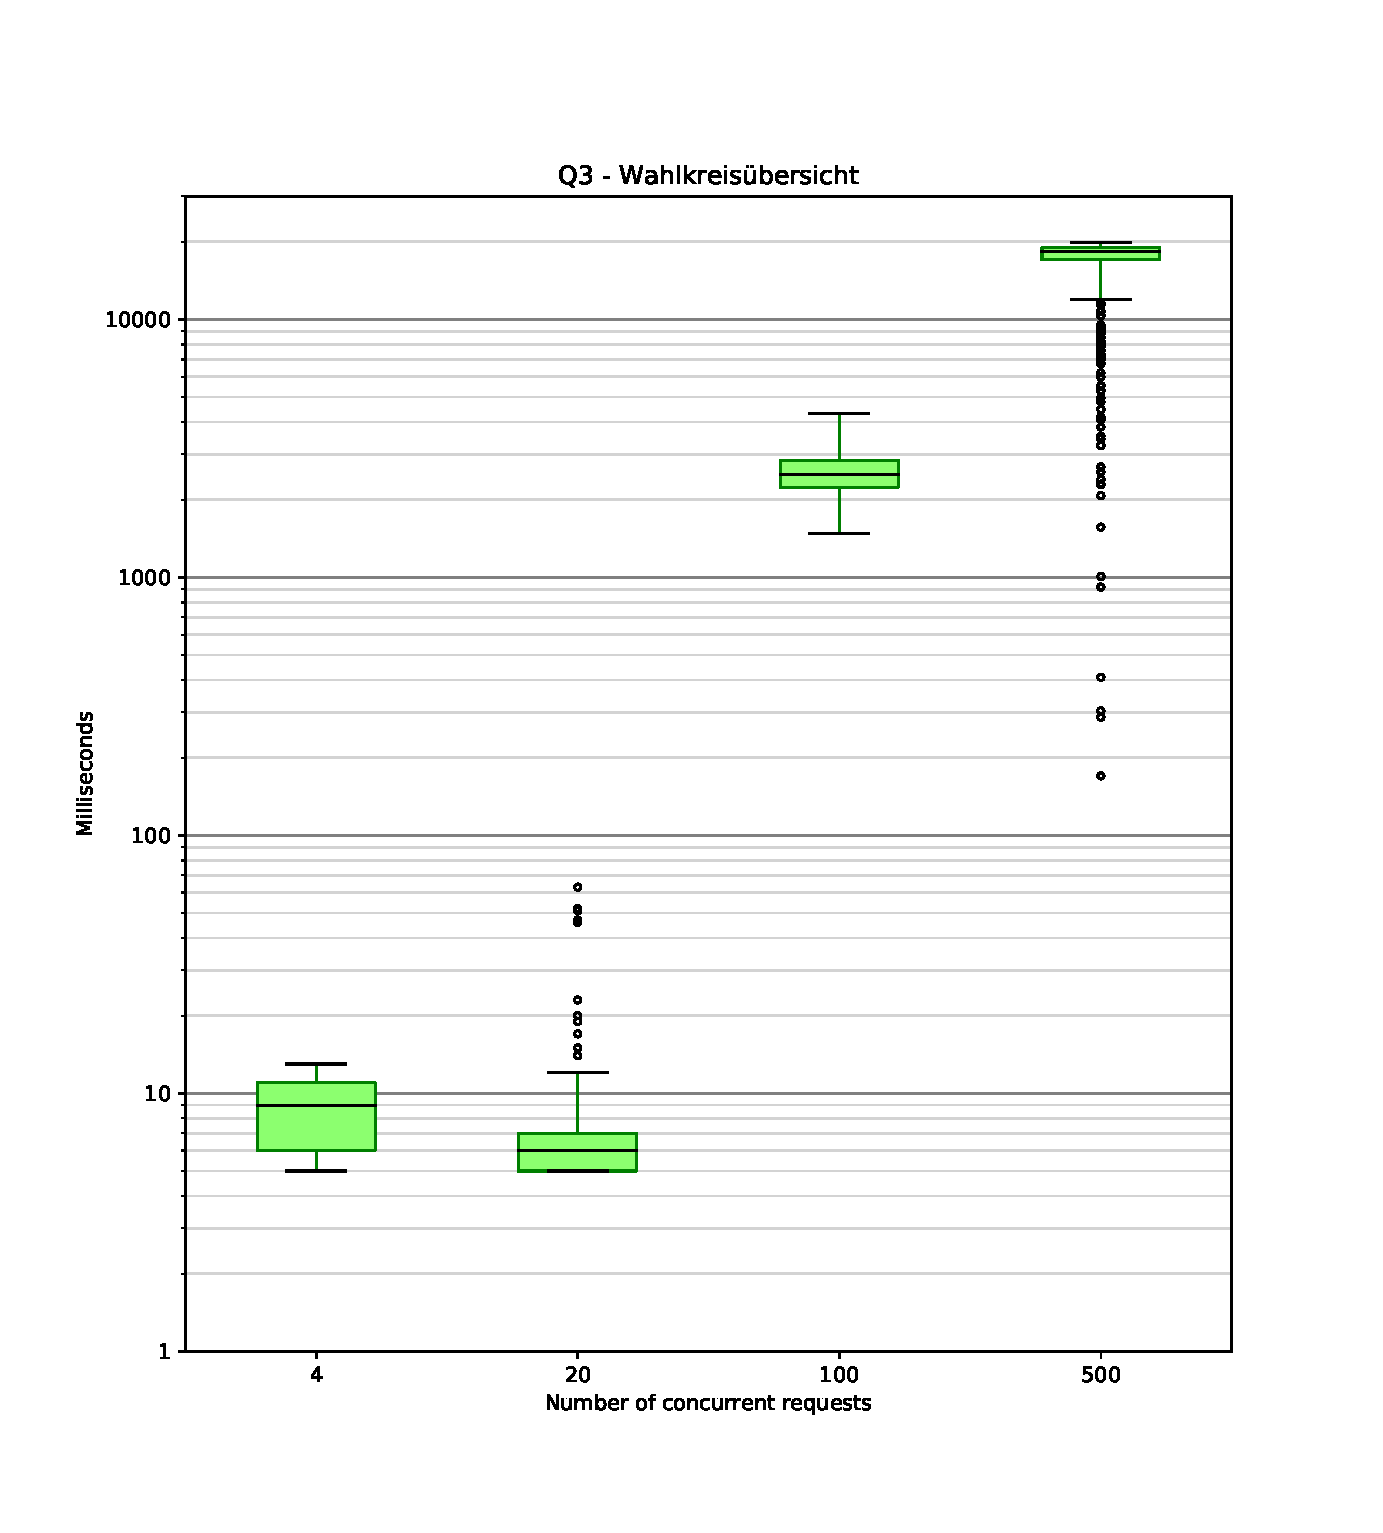
\includegraphics[width=0.9\textwidth]{images/plots_1s/Q3}
	\caption {Q3 - Wahlkreisübersicht (1s)}
\end{figure}

\begin{figure}[htb!]
	\centering
	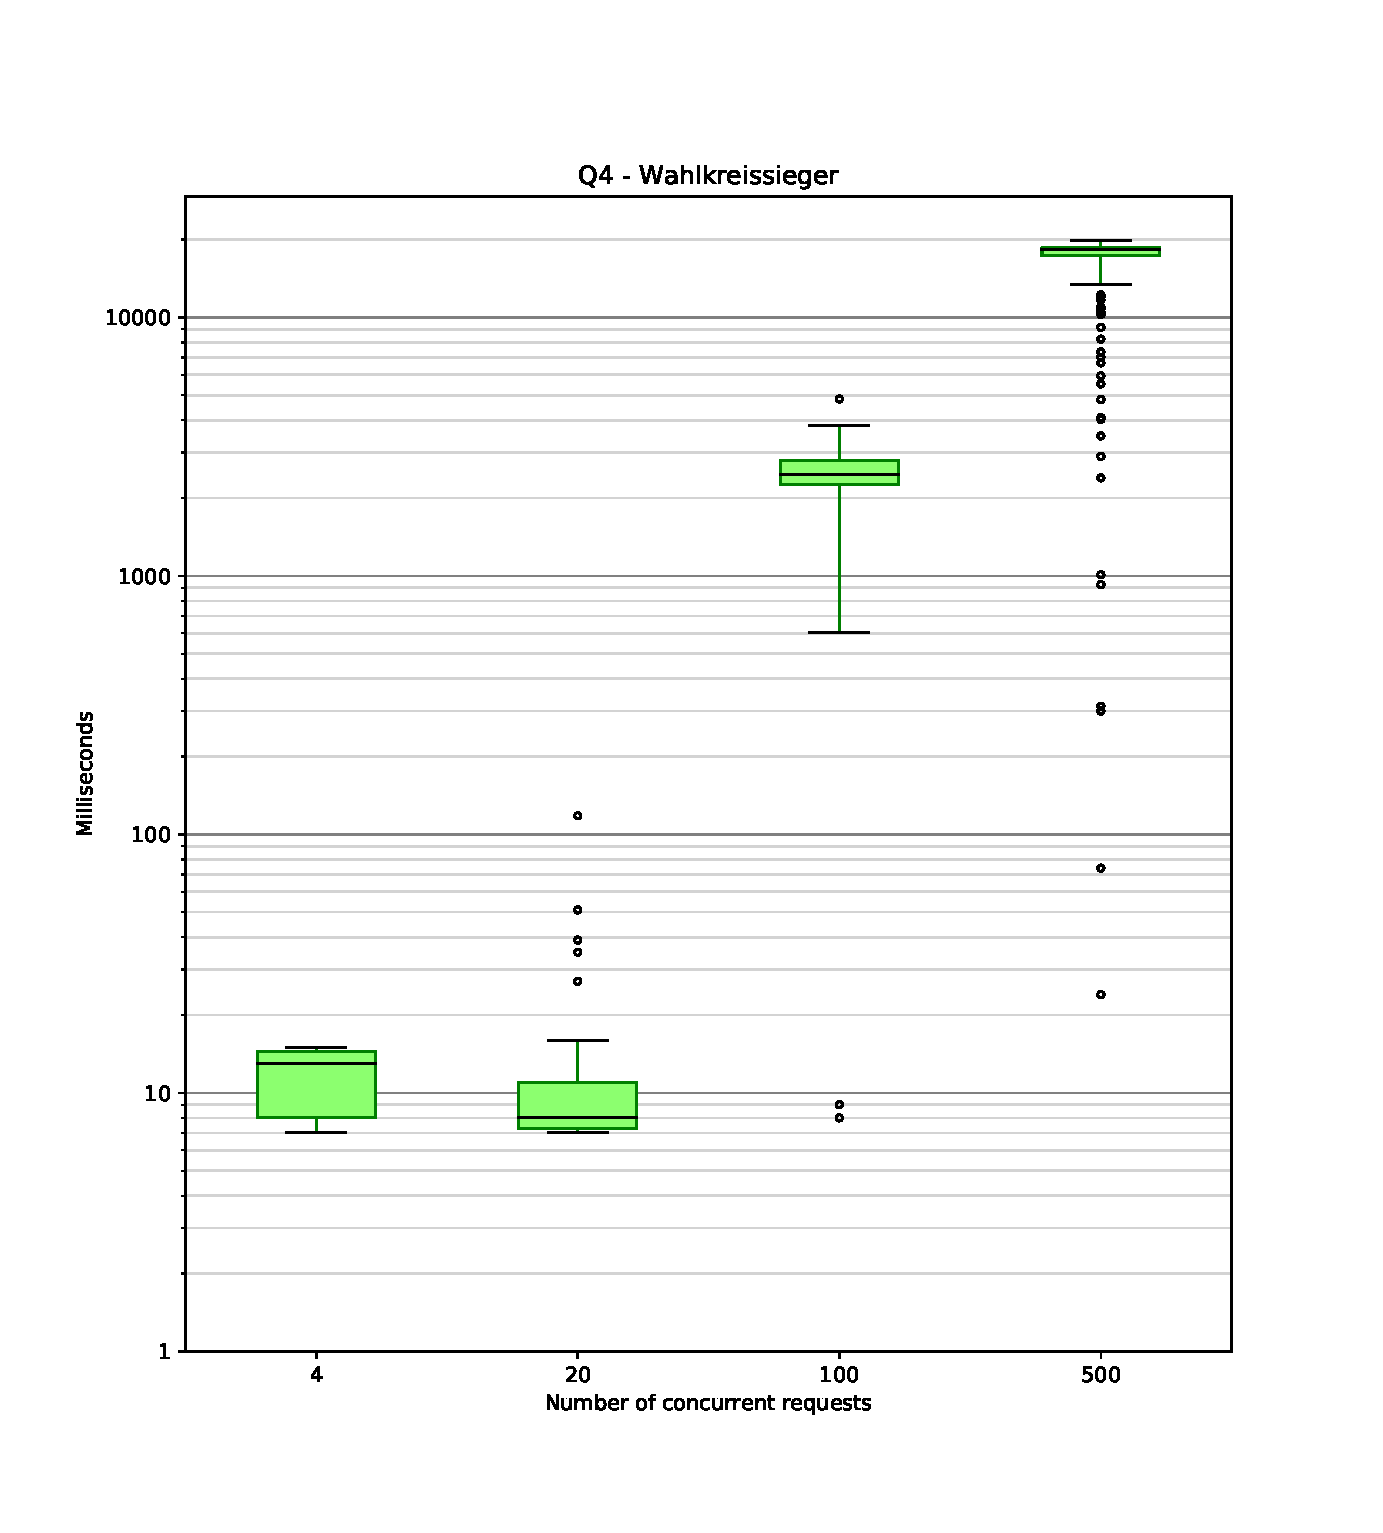
\includegraphics[width=0.9\textwidth]{images/plots_1s/Q4}
	\caption {Q4 - Wahlkreissieger (1s)}
\end{figure}

\begin{figure}[htb!]
	\centering
	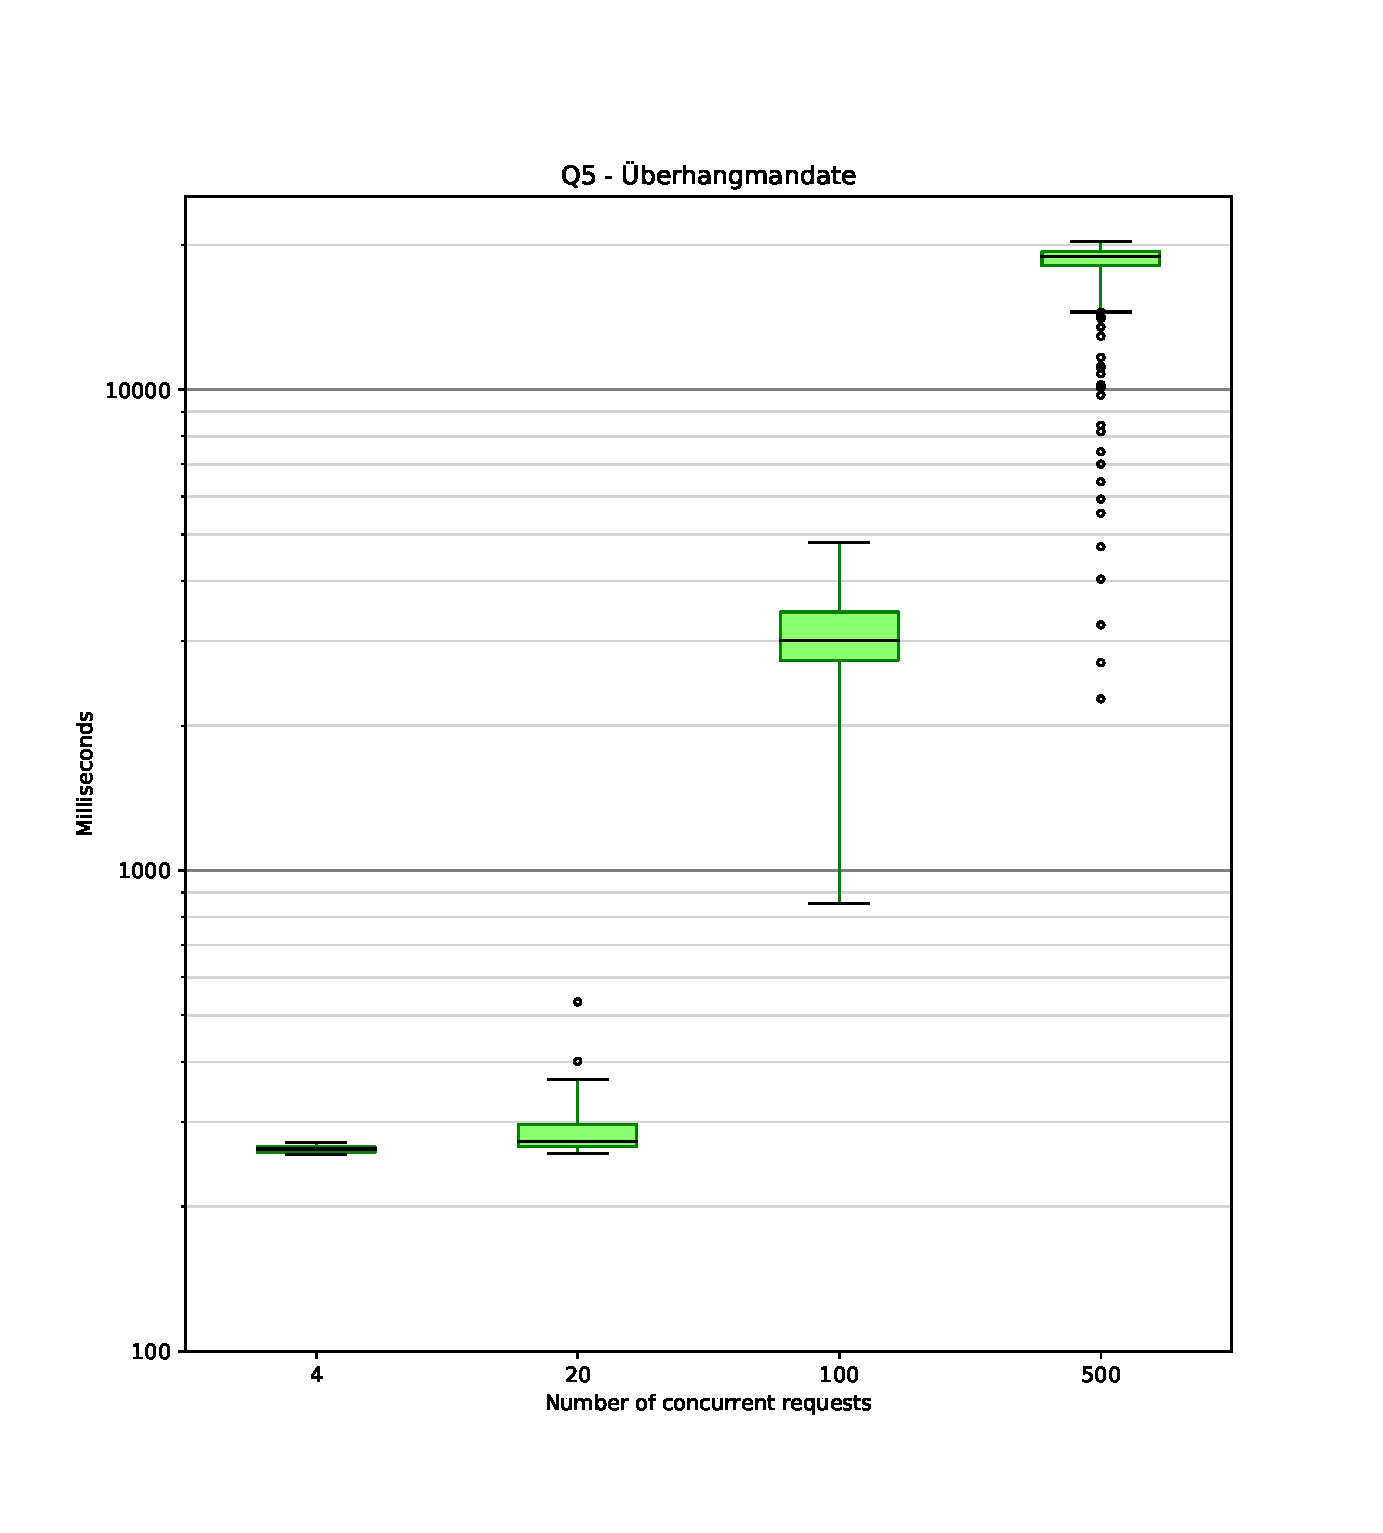
\includegraphics[width=0.9\textwidth]{images/plots_1s/Q5}
	\caption {Q5 - Überhangmandate (1s)}
\end{figure}

\begin{figure}[htb!]
	\centering
	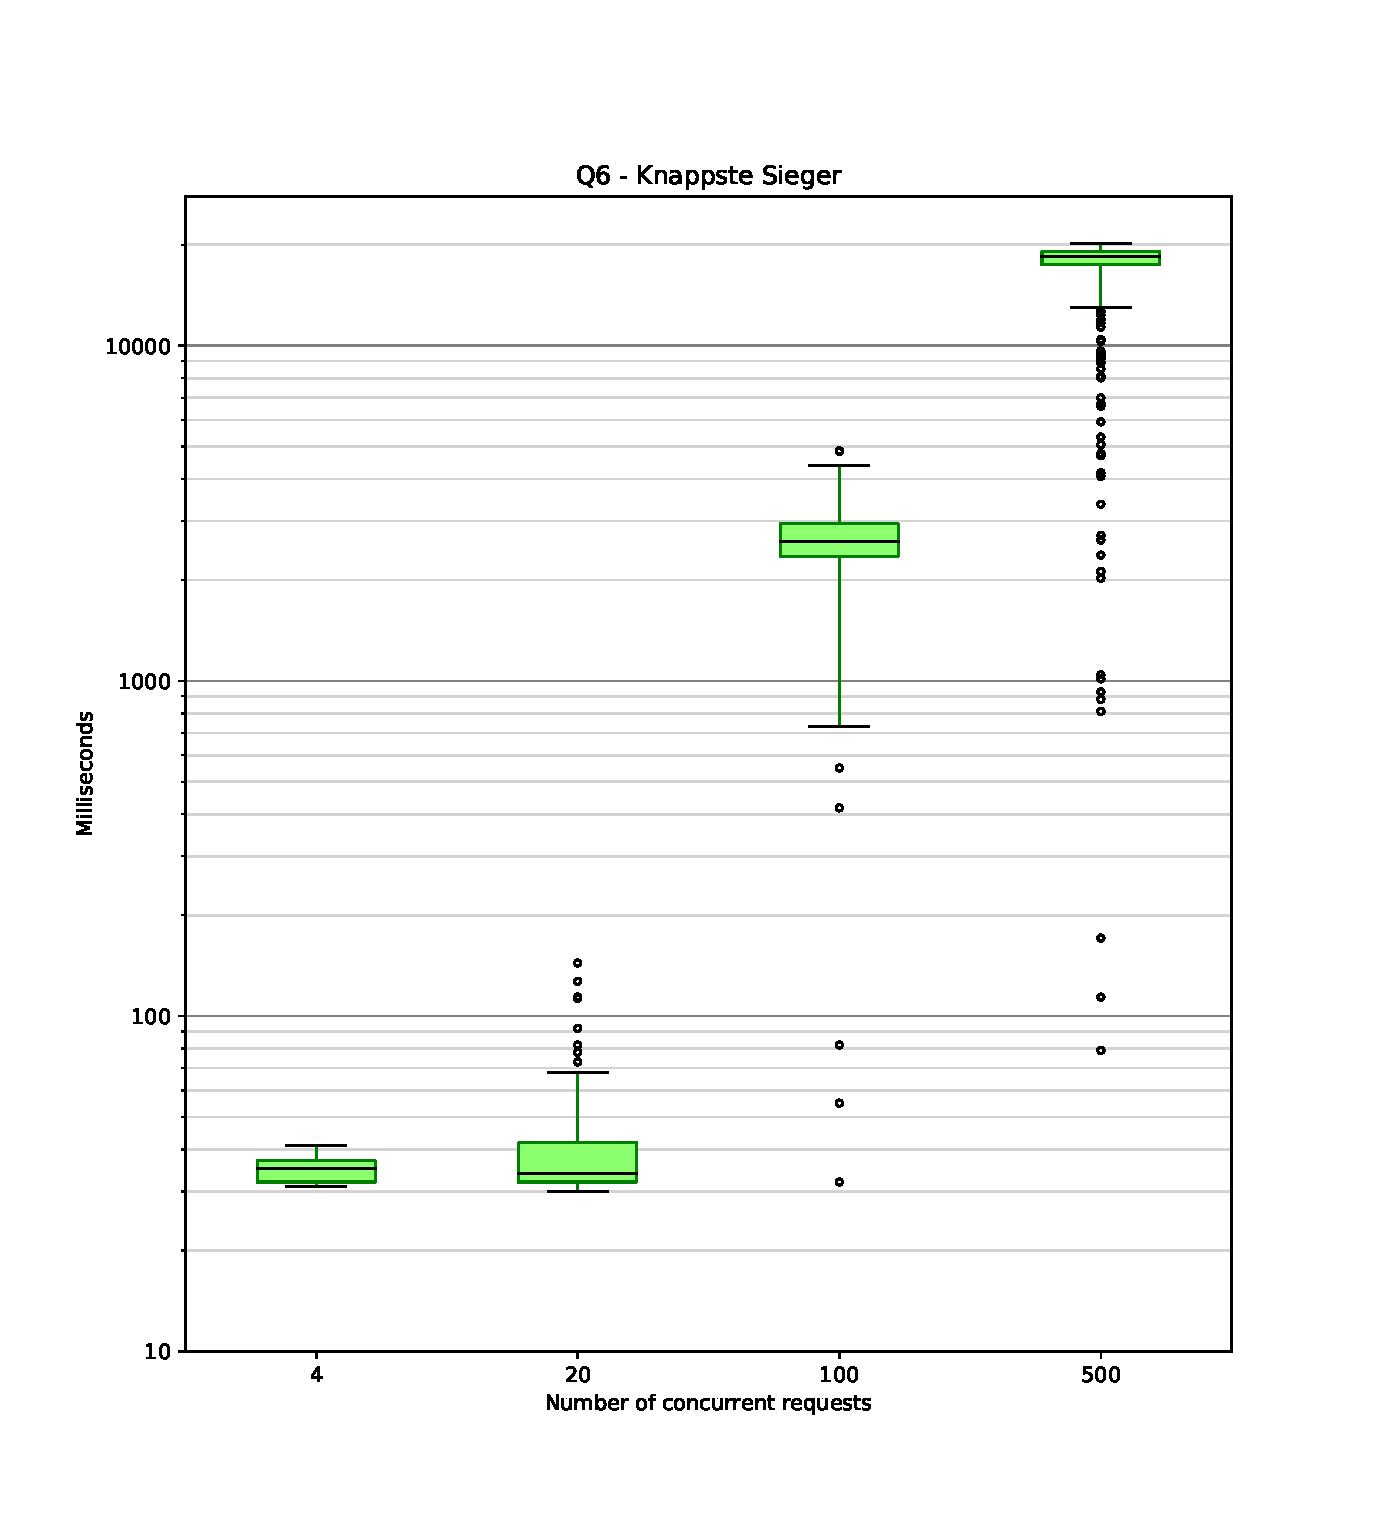
\includegraphics[width=0.9\textwidth]{images/plots_1s/Q6}
	\caption {Q6 - Knappste Sieger (1s)}
\end{figure}

\begin{figure}[htb!]
	\centering
	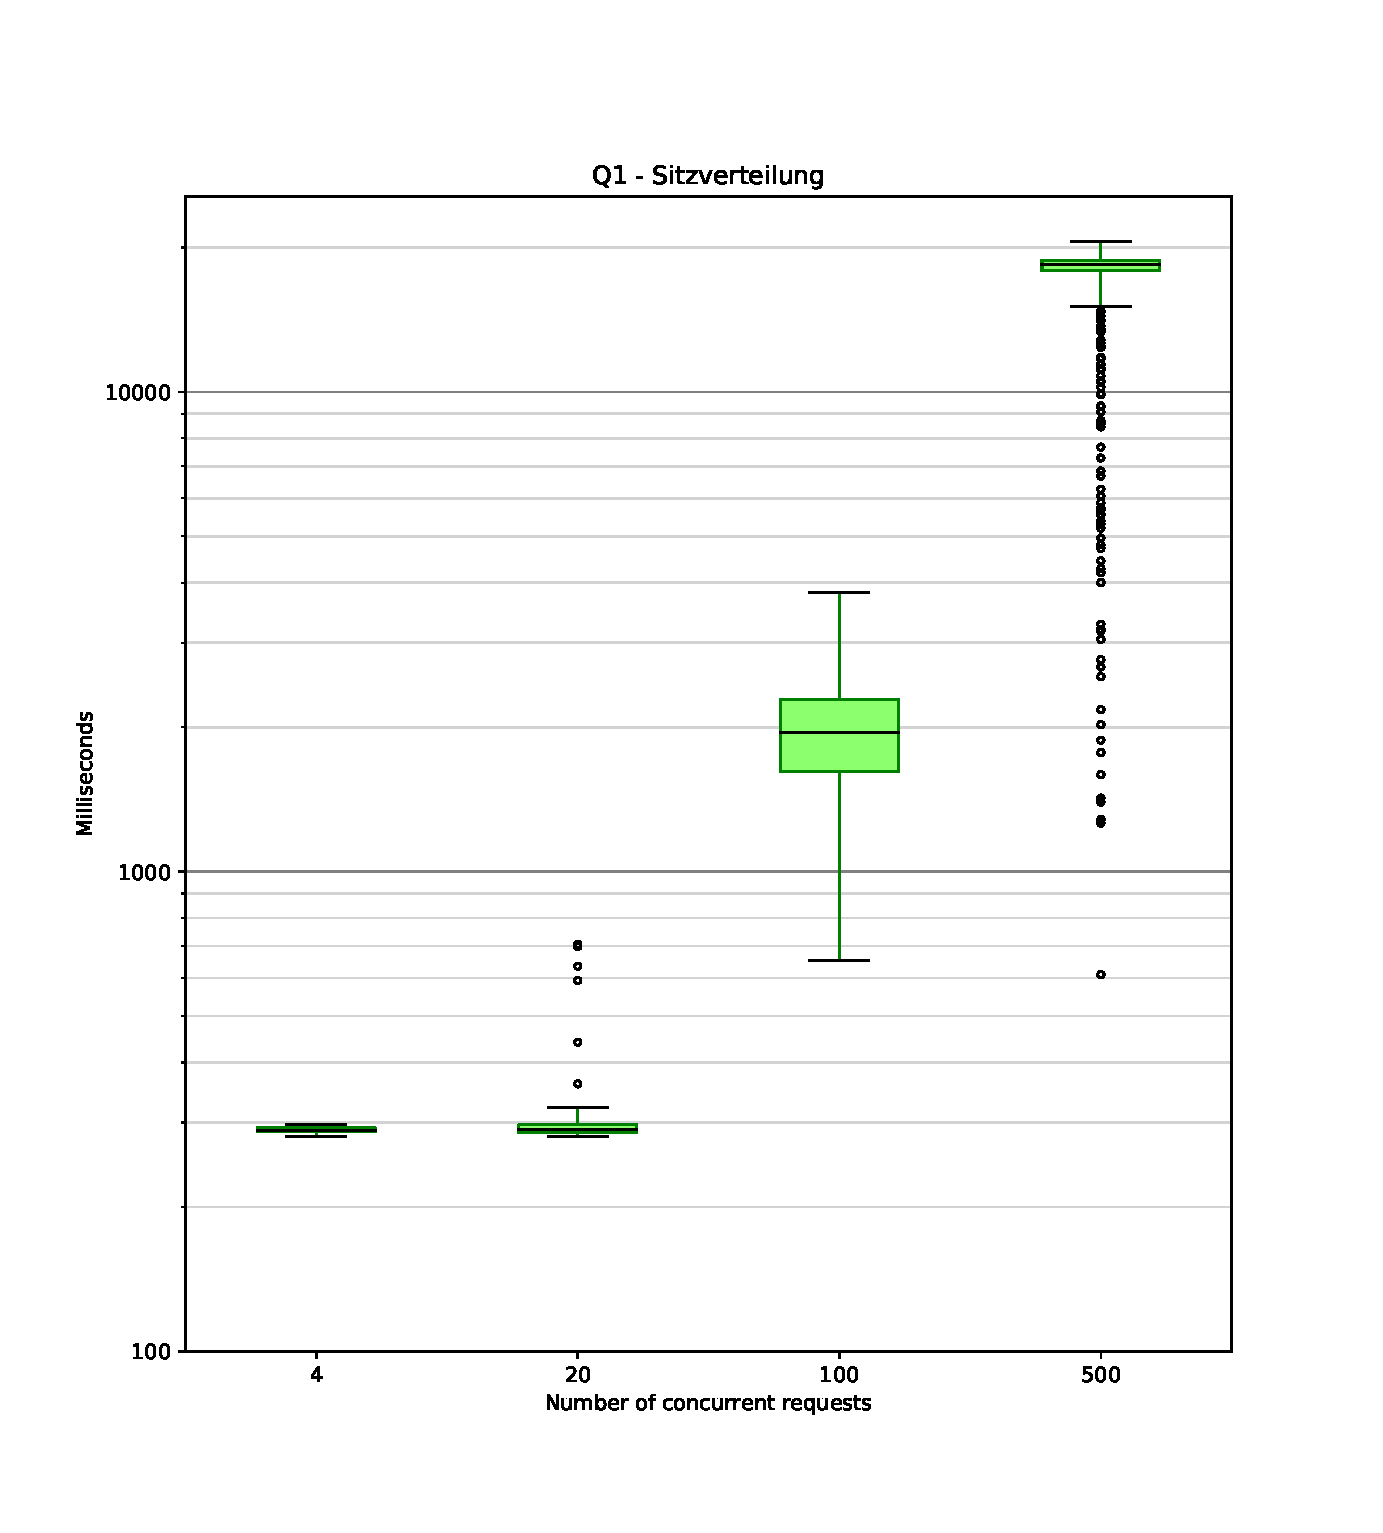
\includegraphics[width=0.9\textwidth]{images/plots_2s/Q1}
	\caption {Q1 - Sitzverteilung (2s)}
\end{figure}

\begin{figure}[htb!]
	\centering
	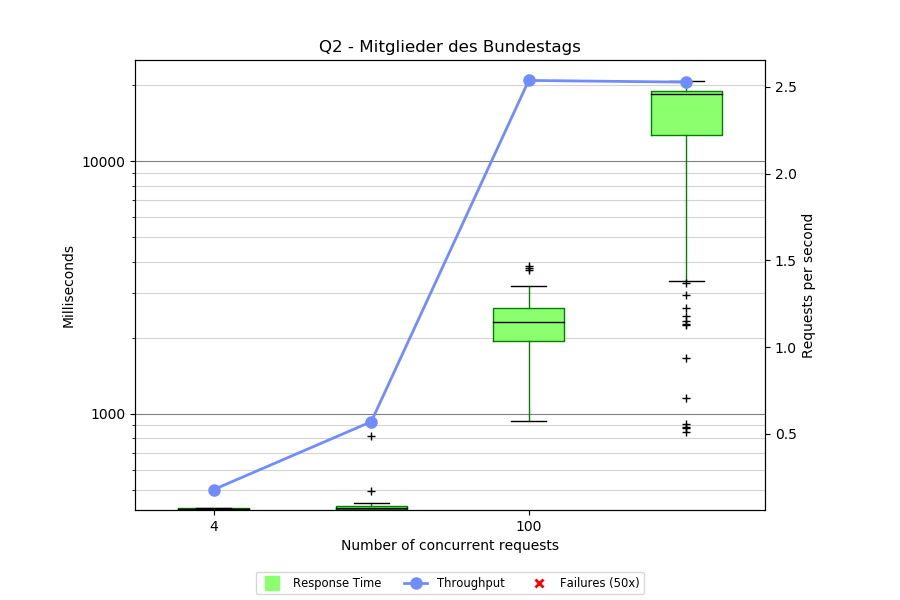
\includegraphics[width=0.9\textwidth]{images/plots_2s/Q2}
	\caption {Q2 - Mitglieder des Bundestags (2s)}
\end{figure}

\begin{figure}[htb!]
	\centering
	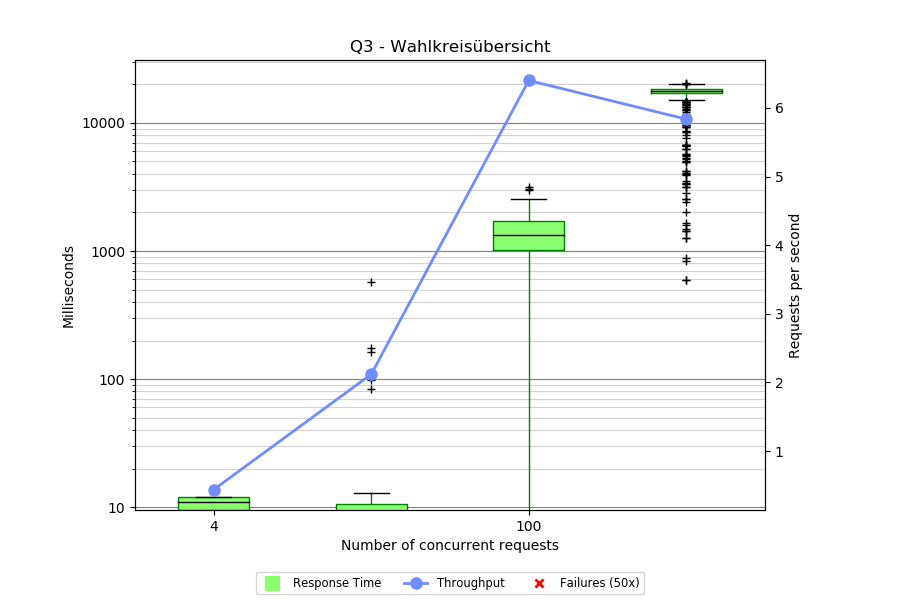
\includegraphics[width=0.9\textwidth]{images/plots_2s/Q3}
	\caption {Q3 - Wahlkreisübersicht (2s)}
\end{figure}

\begin{figure}[htb!]
	\centering
	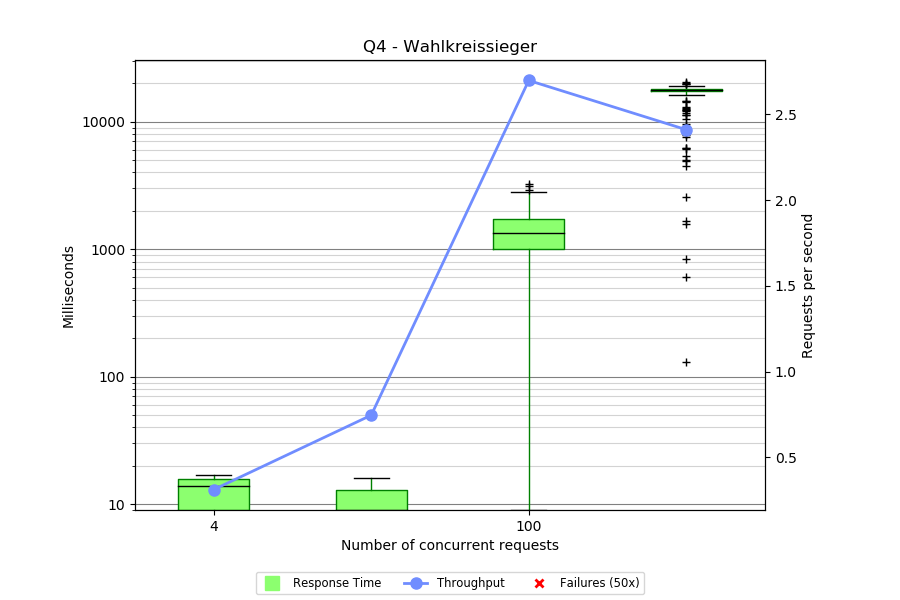
\includegraphics[width=0.9\textwidth]{images/plots_2s/Q4}
	\caption {Q4 - Wahlkreissieger (2s)}
\end{figure}

\begin{figure}[htb!]
	\centering
	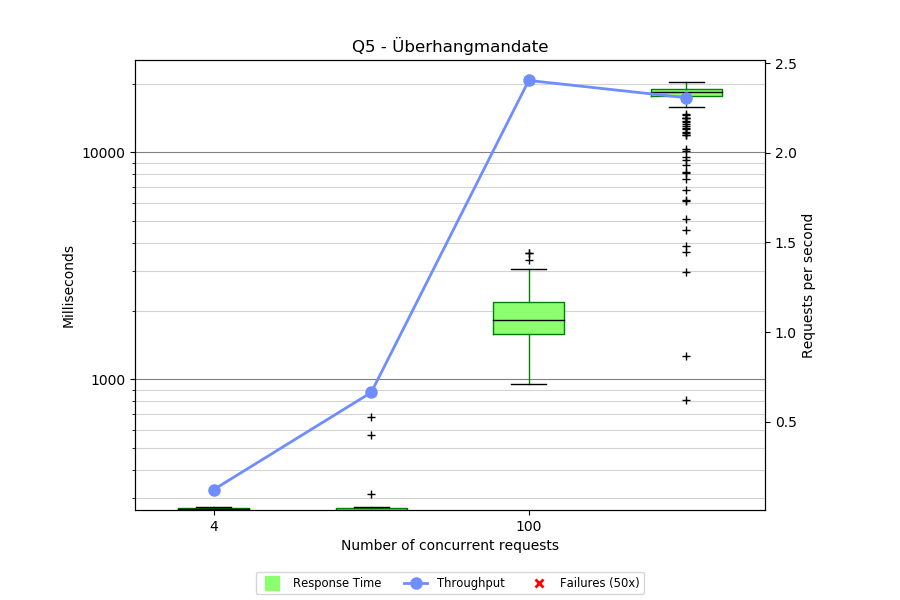
\includegraphics[width=0.9\textwidth]{images/plots_2s/Q5}
	\caption {Q5 - Überhangmandate (2s)}
\end{figure}

\begin{figure}[htb!]
	\centering
	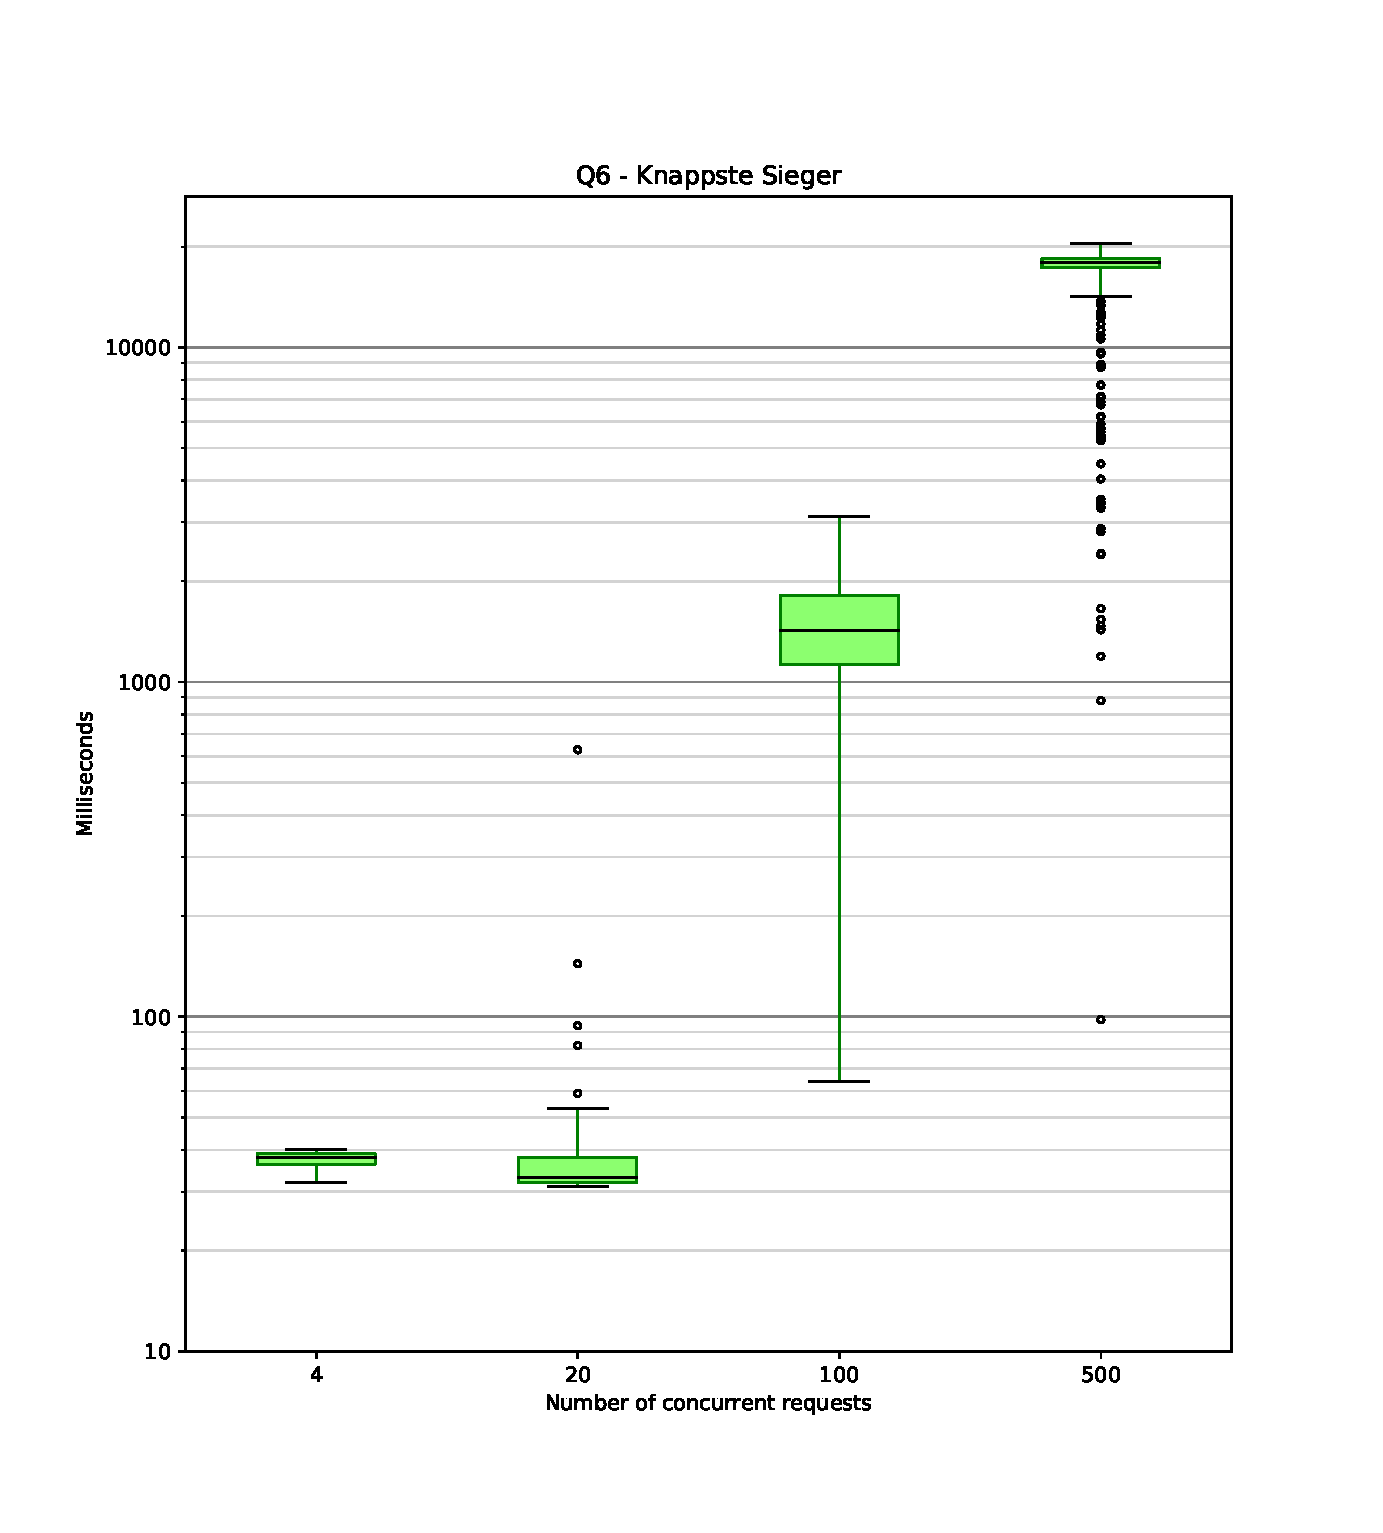
\includegraphics[width=0.9\textwidth]{images/plots_2s/Q6}
	\caption {Q6 - Knappste Sieger (2s)}
\end{figure}

\begin{figure}[htb!]
	\centering
	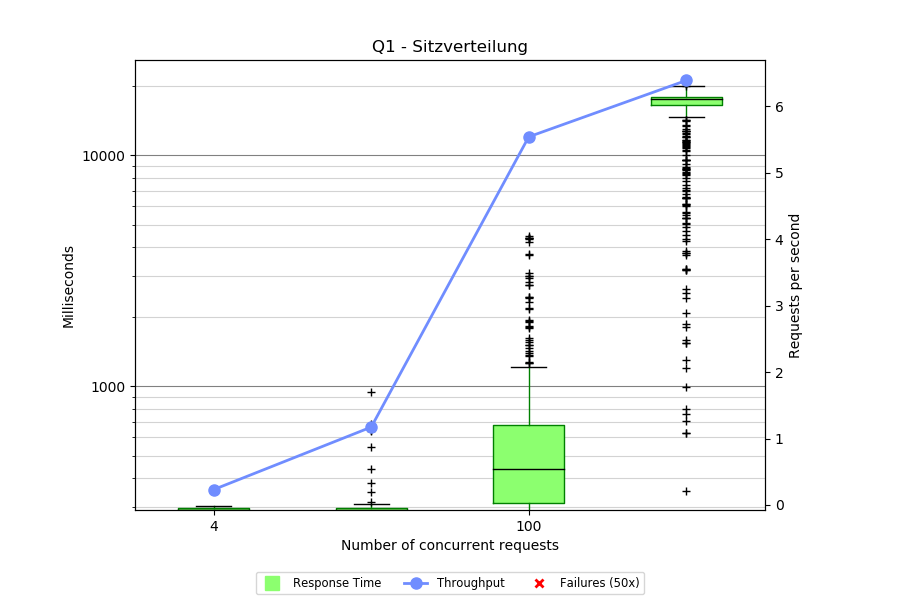
\includegraphics[width=0.9\textwidth]{images/plots_4s/Q1}
	\caption {Q1 - Sitzverteilung (4s)}
\end{figure}

\begin{figure}[htb!]
	\centering
	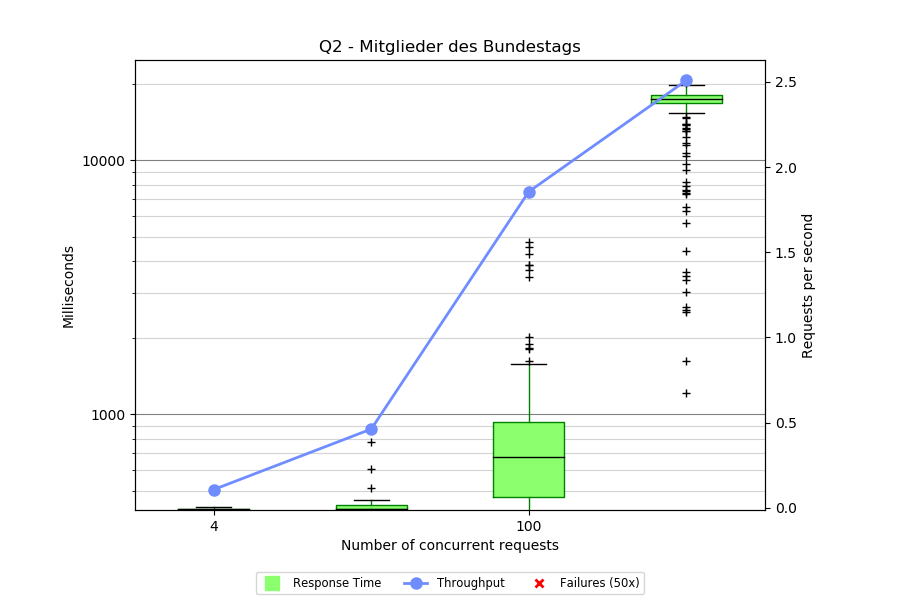
\includegraphics[width=0.9\textwidth]{images/plots_4s/Q2}
	\caption {Q2 - Mitglieder des Bundestags (4s)}
\end{figure}

\begin{figure}[htb!]
	\centering
	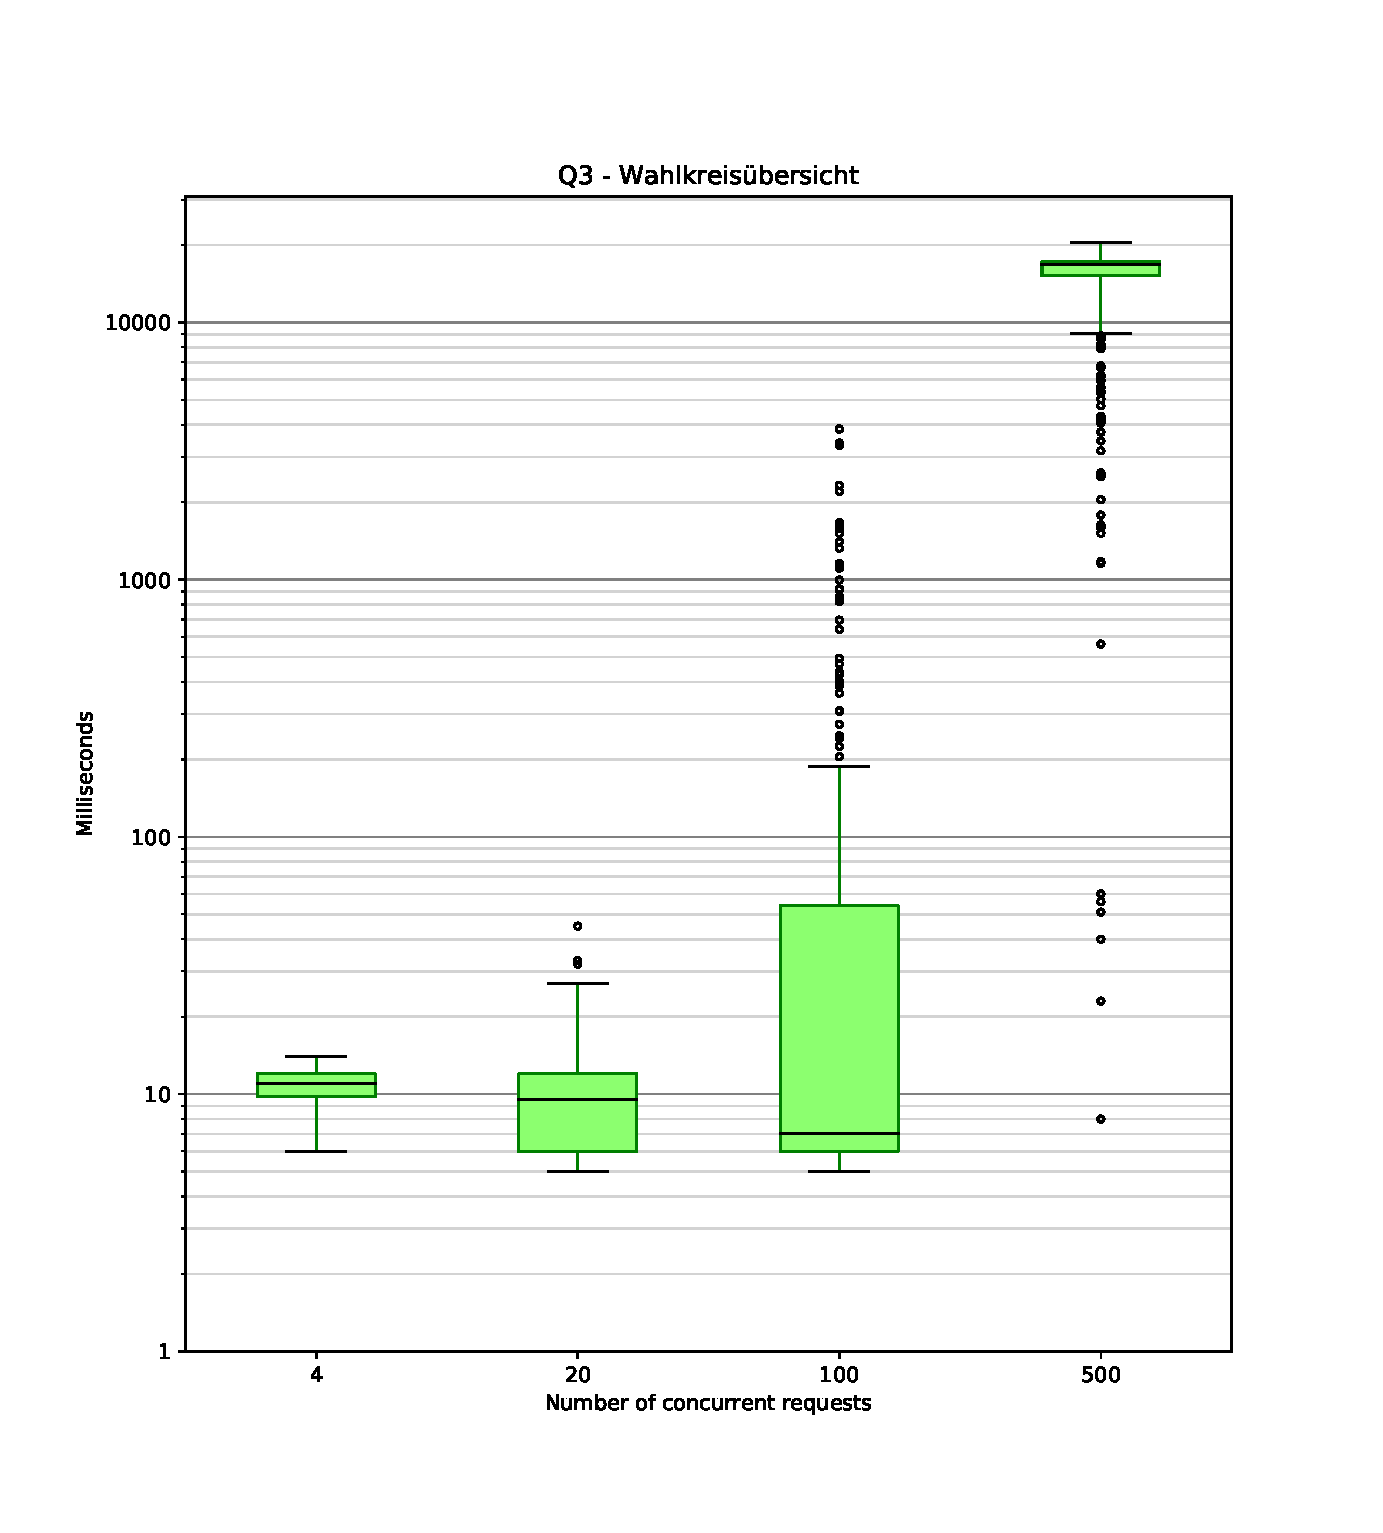
\includegraphics[width=0.9\textwidth]{images/plots_4s/Q3}
	\caption {Q3 - Wahlkreisübersicht (4s)}
\end{figure}

\begin{figure}[htb!]
	\centering
	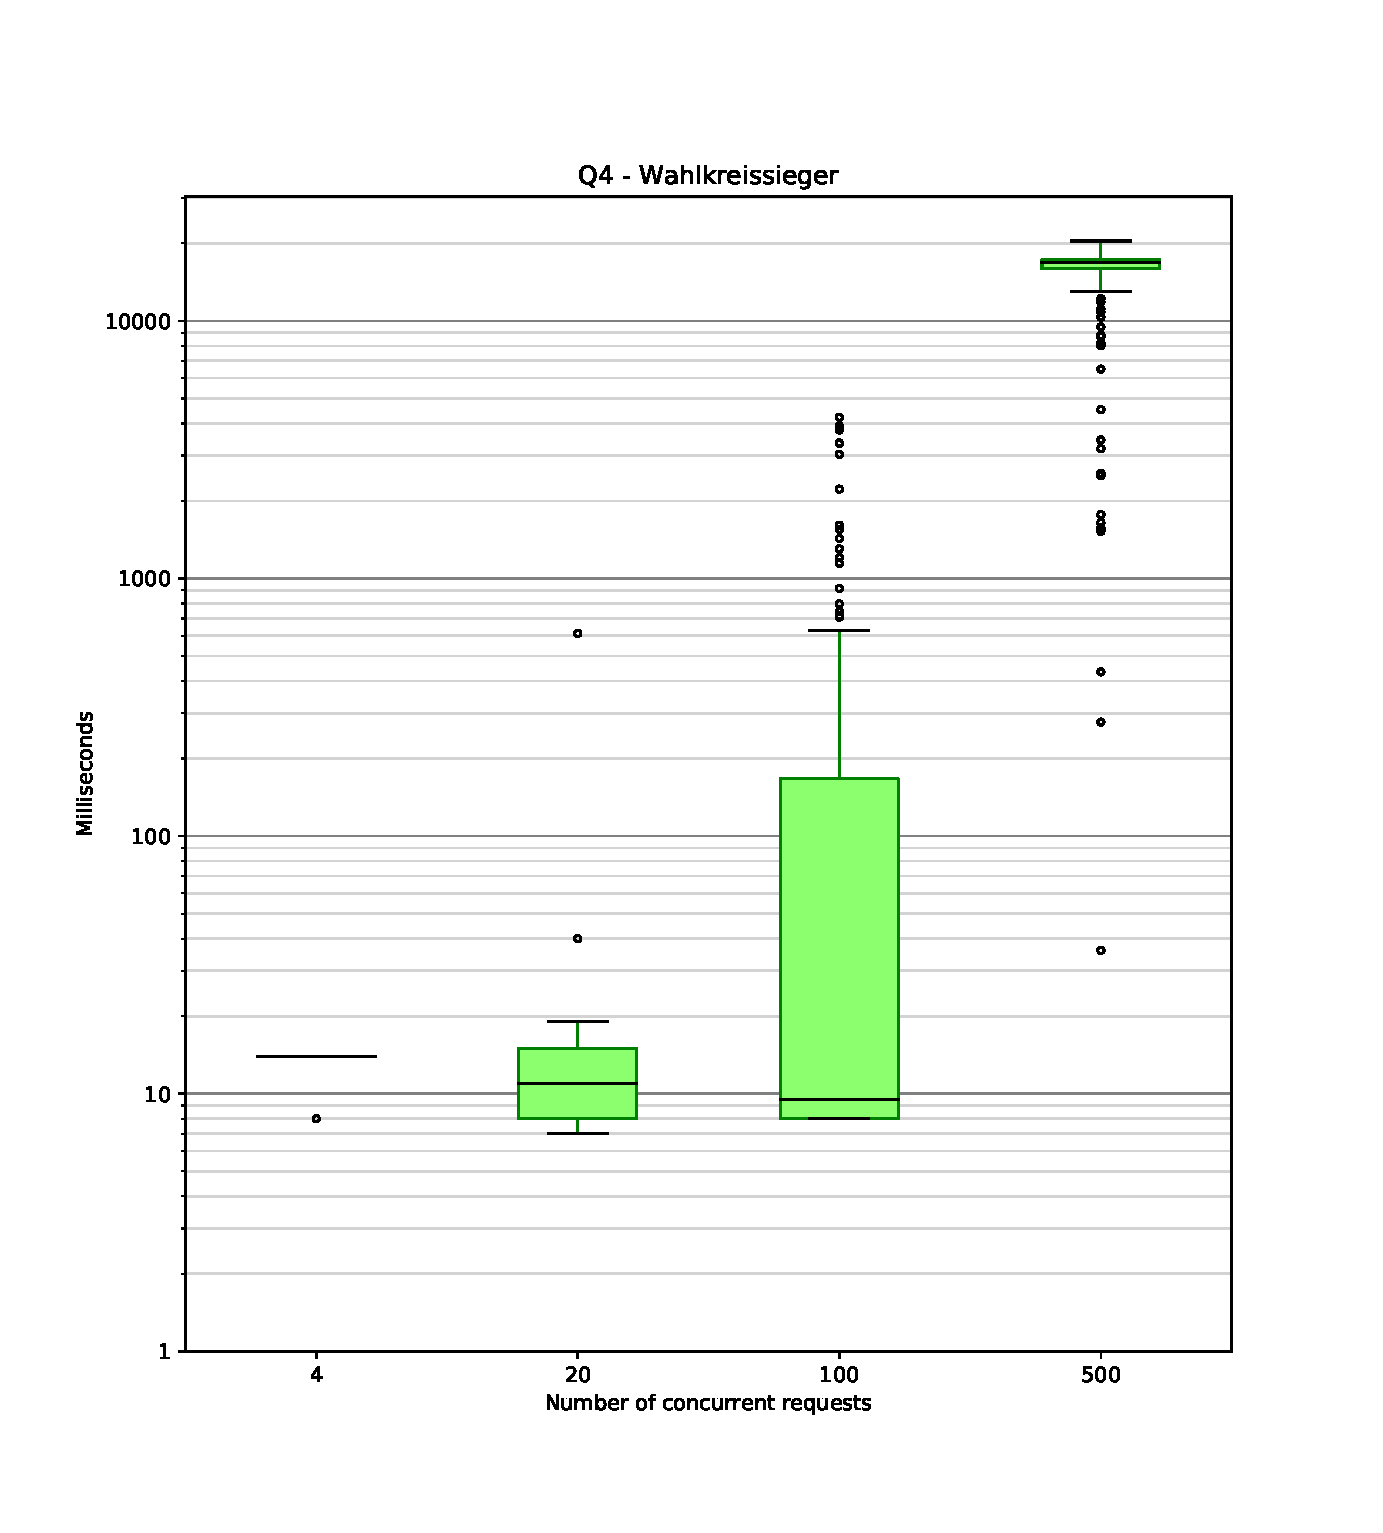
\includegraphics[width=0.9\textwidth]{images/plots_4s/Q4}
	\caption {Q4 - Wahlkreissieger (4s)}
\end{figure}

\begin{figure}[htb!]
	\centering
	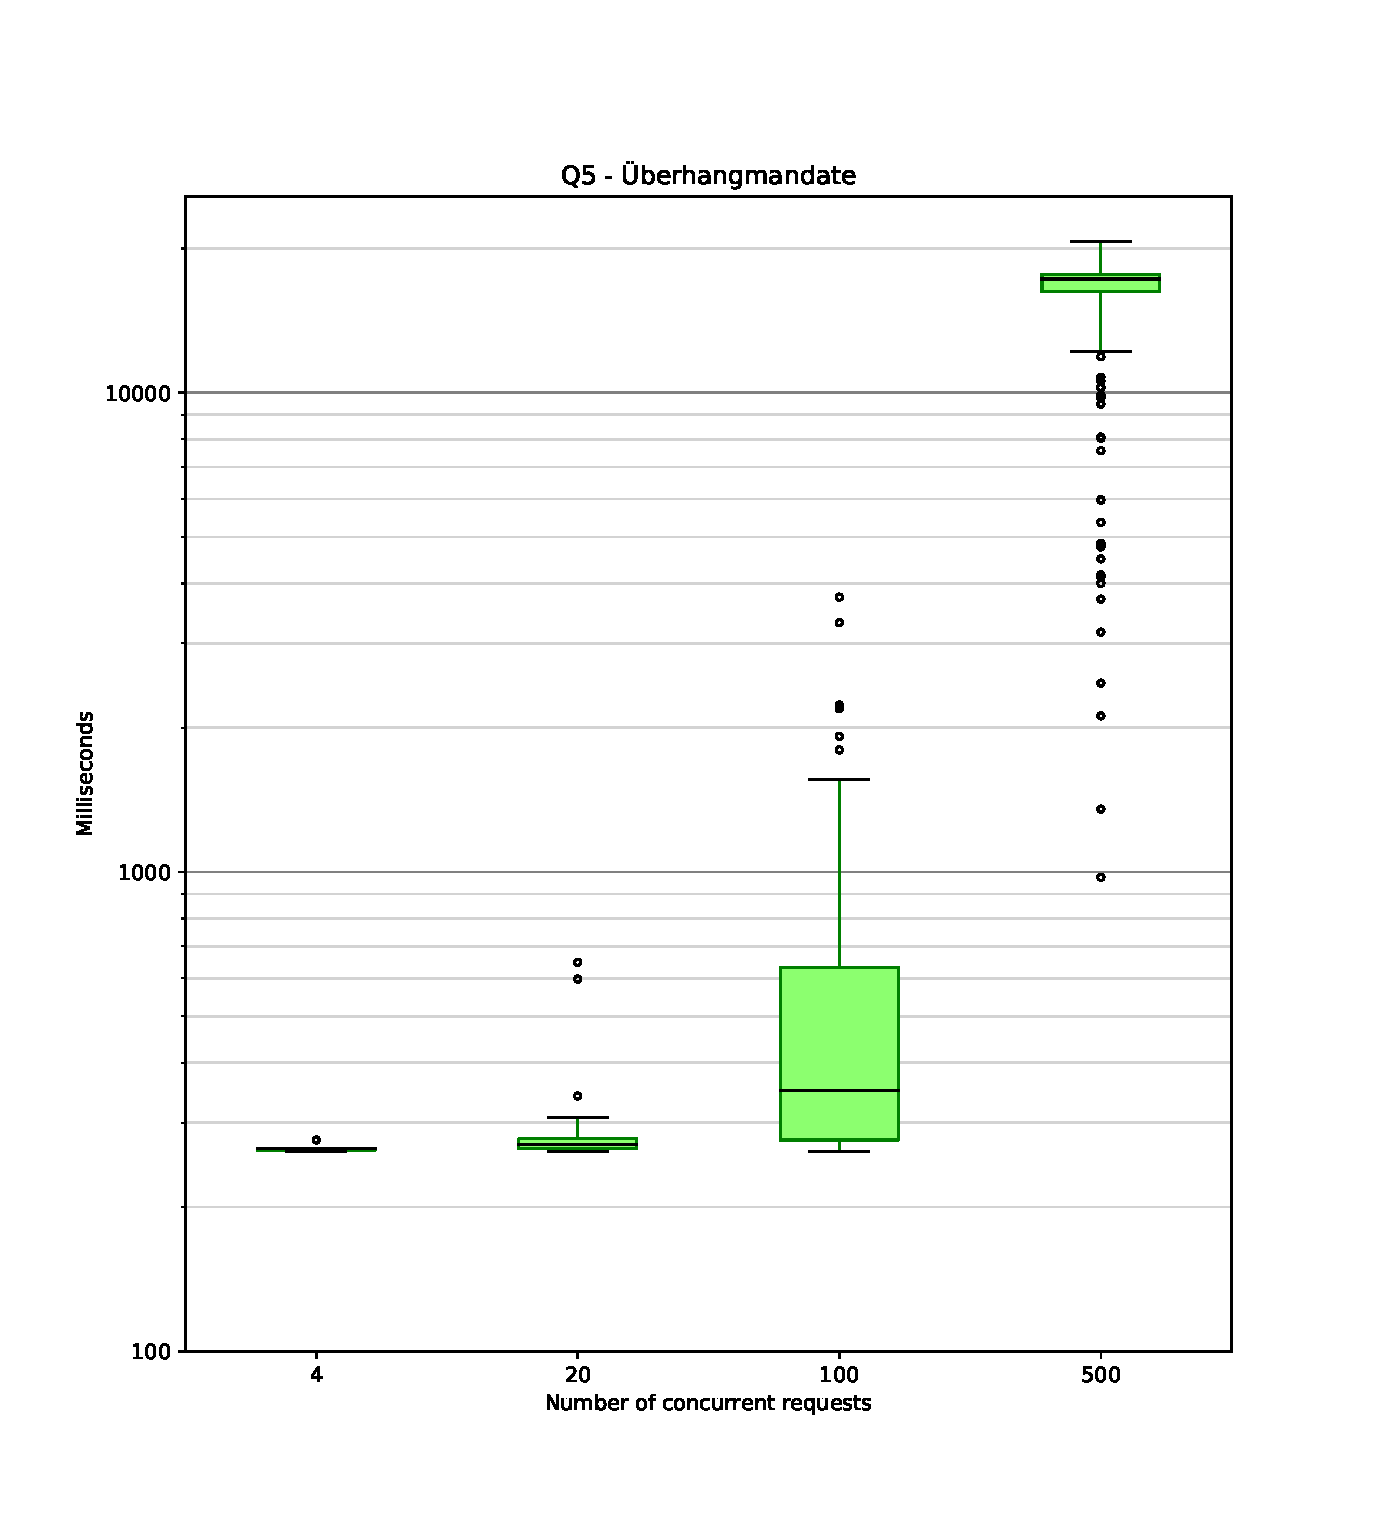
\includegraphics[width=0.9\textwidth]{images/plots_4s/Q5}
	\caption {Q5 - Überhangmandate (4s)}
\end{figure}

\begin{figure}[htb!]
	\centering
	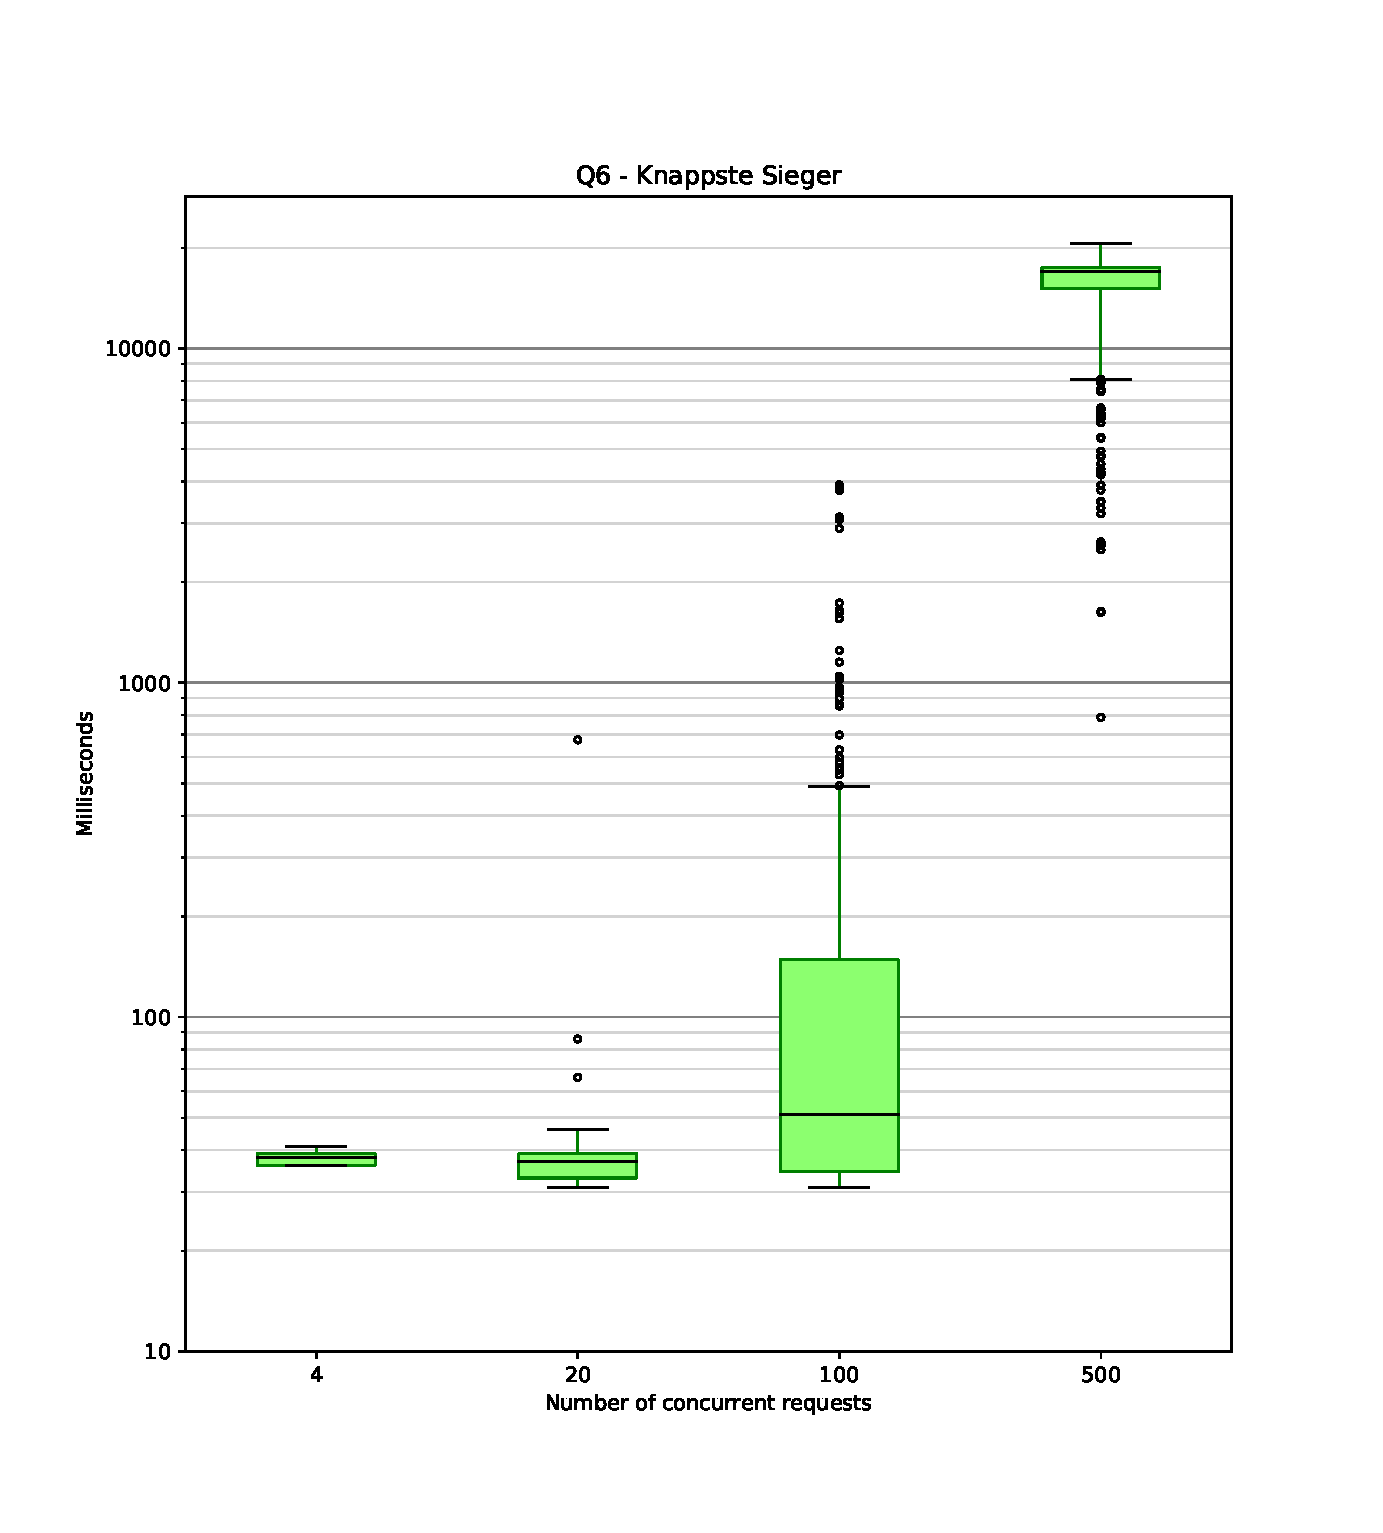
\includegraphics[width=0.9\textwidth]{images/plots_4s/Q6}
	\caption {Q6 - Knappste Sieger (4s)}
\end{figure}


\begin{figure}[htb!]
	\centering
	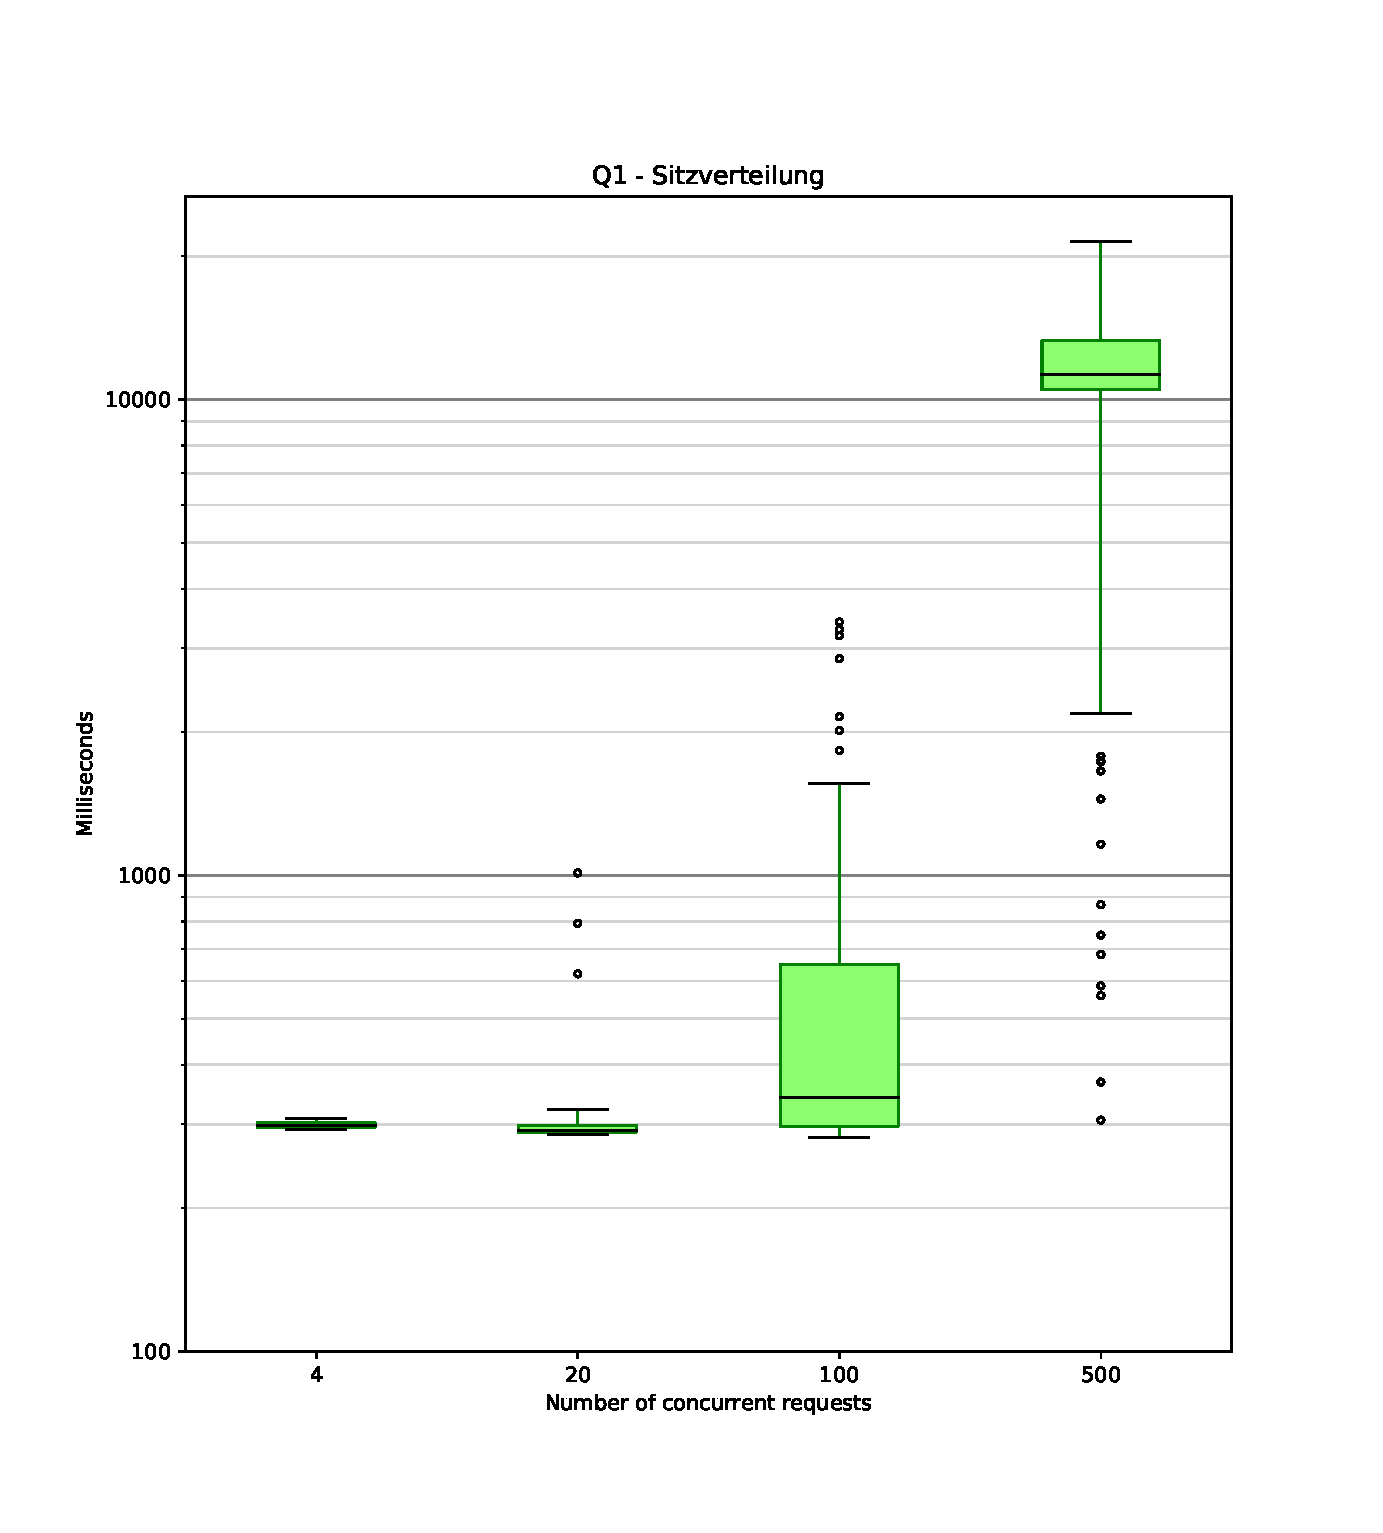
\includegraphics[width=0.9\textwidth]{images/plots_8s/Q1}
	\caption {Q1 - Sitzverteilung (8s)}
\end{figure}

\begin{figure}[htb!]
	\centering
	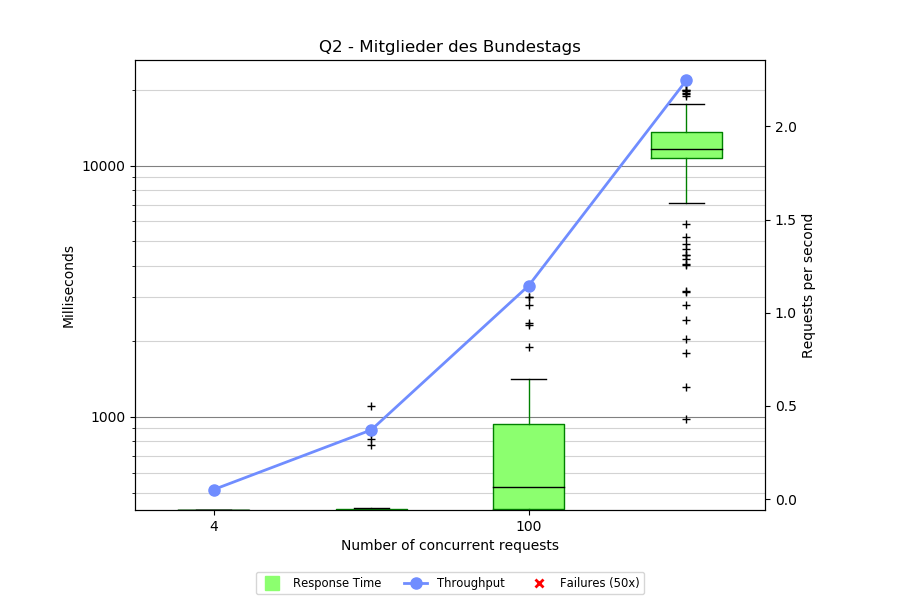
\includegraphics[width=0.9\textwidth]{images/plots_8s/Q2}
	\caption {Q2 - Mitglieder des Bundestags (8s)}
\end{figure}

\begin{figure}[htb!]
	\centering
	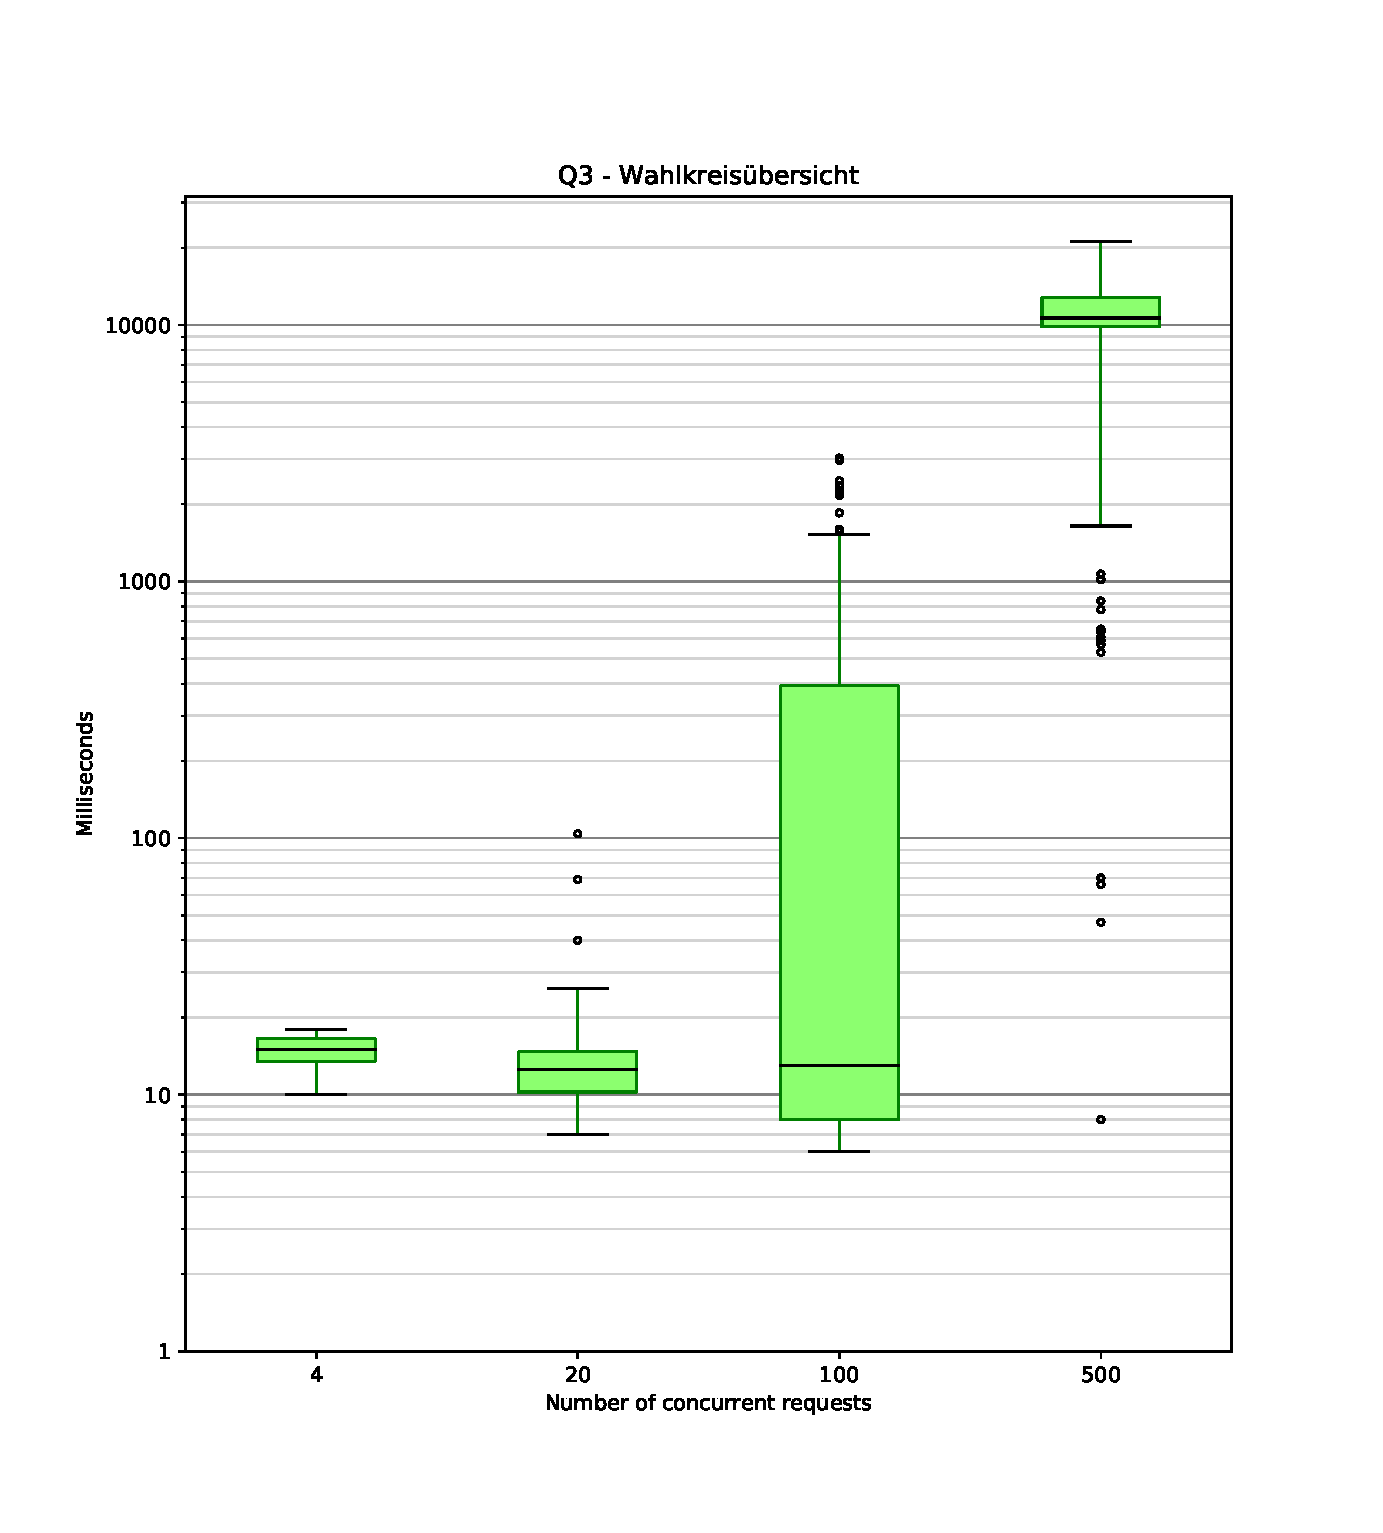
\includegraphics[width=0.9\textwidth]{images/plots_8s/Q3}
	\caption {Q3 - Wahlkreisübersicht (8s)}
\end{figure}

\begin{figure}[htb!]
	\centering
	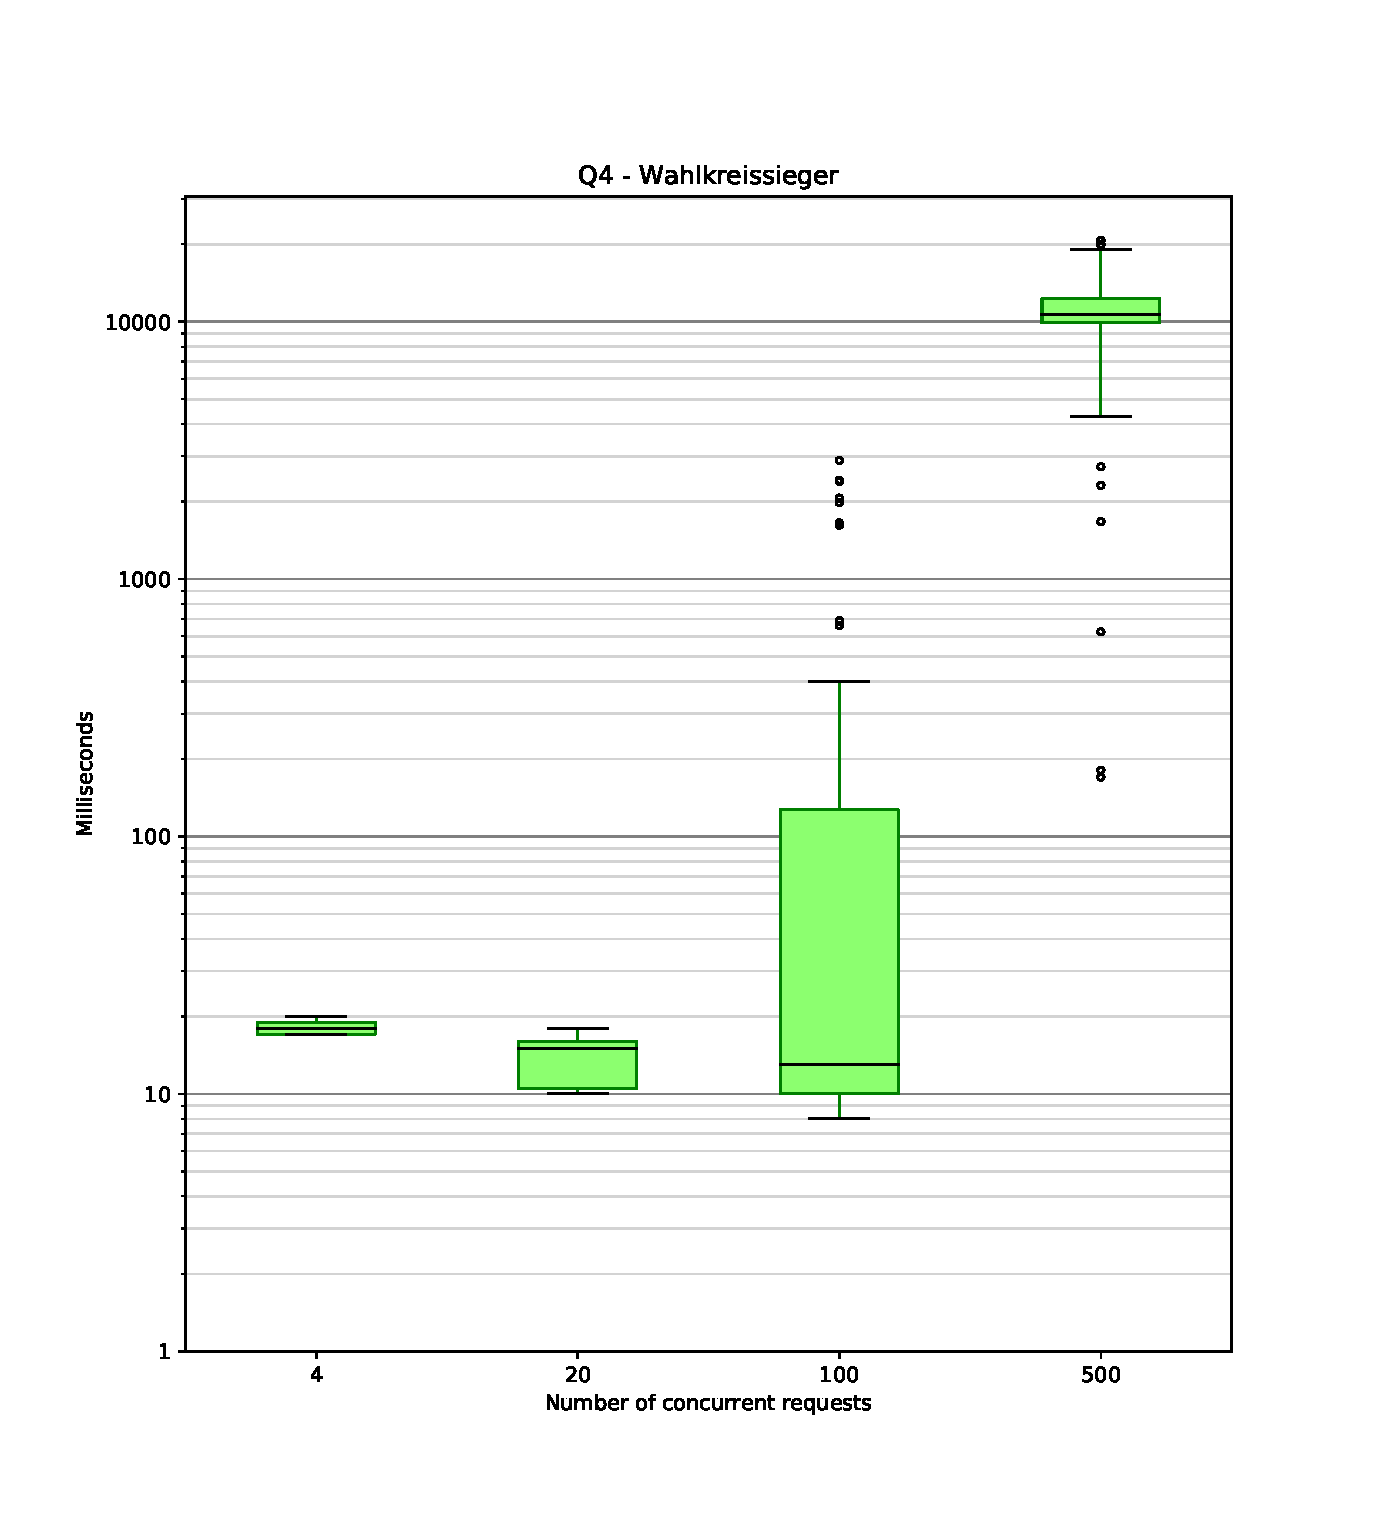
\includegraphics[width=0.9\textwidth]{images/plots_8s/Q4}
	\caption {Q4 - Wahlkreissieger (8s)}
\end{figure}

\begin{figure}[htb!]
	\centering
	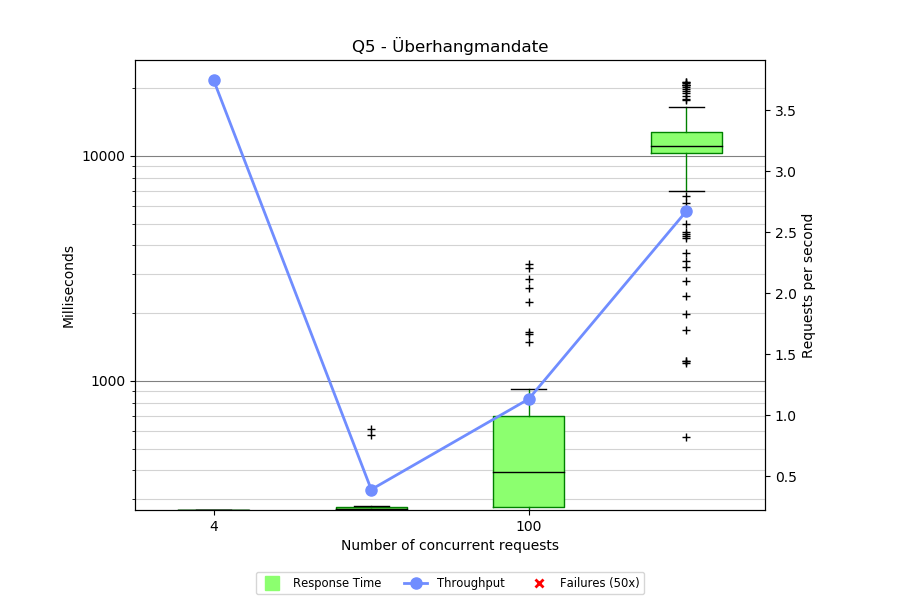
\includegraphics[width=0.9\textwidth]{images/plots_8s/Q5}
	\caption {Q5 - Überhangmandate (8s)}
\end{figure}

\begin{figure}[htb!]
	\centering
	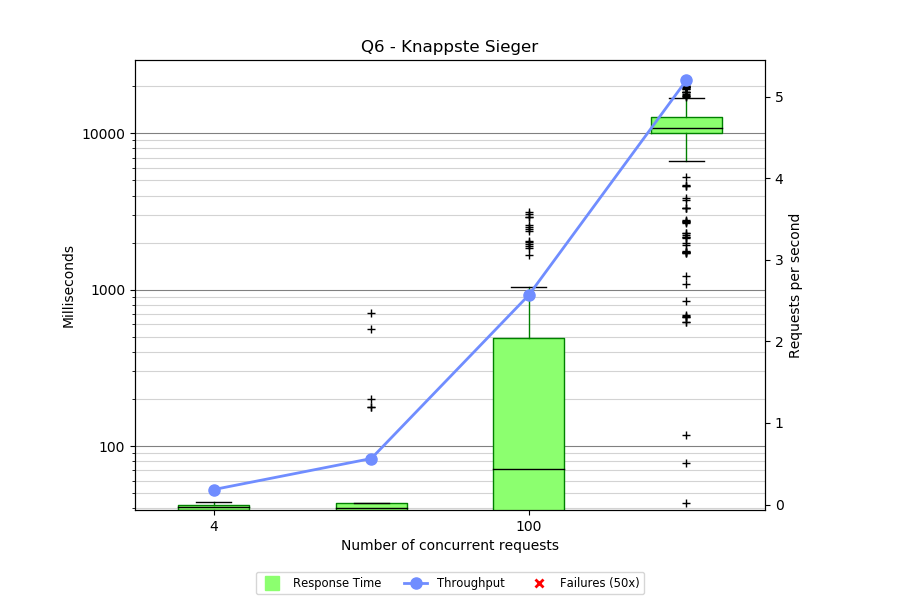
\includegraphics[width=0.9\textwidth]{images/plots_8s/Q6}
	\caption {Q6 - Knappste Sieger (8s)}
\end{figure}



% Glossar
\newglossaryentry{betreiber}{
  name=Betreiber,
  description={Die Person oder Rechtsperson, die für die Installation und den Betrieb des \gls{system}s verantwortlich ist}
}
\newglossaryentry{system}{
  name=System,
  description={Die Gesamtheit der ausgelieferten Software in einer \gls{systemumgebung}}
}
\newglossaryentry{systemumgebung}{
  name=Systemumgebung,
  description={Alle Soft- und Hardware, die zum Betrieb des \gls{system}s benötigt wird, aber nicht mit dem \gls{system} ausgeliefert wird}
}
\newglossaryentry{stimme}{
  name=Stimme,
  description={Eine konkrete Instanz der Einflussnahme eines deutschen Staatsbürgers durch Abgabe einer Stimme nach dem deutschen Wahlrecht, bestehend aus Erst- und Zweitstimme},
  plural={Stimmen}
}
\newglossaryentry{einzelstimme}{
  name=Einzelstimme,
  description={Synonym für \gls{stimme}, mit Betonung der Abgrenzung von \gls{akku-stimme}}
}
\newglossaryentry{akku-stimme}{
  name=akkumulierte Stimmen,
  description={Die Zusammenfassung mehrerer \glspl{stimme}. Diese besteht aus absoluten Zahlen und enthält die Anzahl der abgegebenen Erststimmen pro Kandidat, die Anzahl der abgegebenen Zweitstimmen pro Landesliste. Falls über eine abstrakte Wählergruppe akkumuliert wird und nicht über eine Menge konkreter Stimmen, sind außerdem die Anzahl der ungültigen \glspl{stimme} und die Anzahl der Wahlberechtigten (oder die Anzahl der sog. Nichtwähler) in der Wählergruppe enthalten}
}
\newglossaryentry{sicherheitscode}{
  name=Sicherheitscode,
  description={Eine Zeichenkette, die zur Autorisierung geeignet ist. Mit einem Sicherheitscode kann -- abhängig von der Bestimmung des Codes -- entweder das Abgeben einer einzelnen Stimme im Wahllokal oder das Eintragen von \gls{akku-stimme} im \gls{system} autorisiert werden}
}
\newglossaryentry{uptime}{
  name=Uptime,
  description={Die summierte Zeit, prozentual gemessen an einer konkreten Zeitspanne, zu der das \gls{system} einsatzfähig ist.}
}
\glsaddall
\printglossary
 
% Abbildungsverzeichnis
%\listoffigures
 
\end{document}